%% \documentclass[handout,t]{beamer} % HANDOUT
%% \documentclass[handout,notes=show,t]{beamer} % NOTES
\documentclass[t]{beamer} % SLIDES

\usetheme{ZipfR}
\usepackage{beamer-tools}

%%
%%  INCLUDE: math.tex
%%  
%%  basic mathematical symbols and constructs (not specific to cooccurrences)
%%


%% \setN, \setN[0], \setZ, \setQ, \setR, \setC
%% abbreviations for common number spaces
\newcommand{\setN}[1][]{\mathbb{N}_{#1}} % allows \setN and \setN[0]
\newcommand{\setZ}{\mathbb{Z}}
\newcommand{\setQ}{\mathbb{Q}}
\newcommand{\setR}{\mathbb{R}}
\newcommand{\setC}{\mathbb{C}}

%% \set{el_1, el_2, ...};  \setdef{el}{condition};  \bigset{..}, \bigsetdef{..}{..}
%% extensional and intensional definition of sets, with "big" versions (like \bigl etc.)
\newcommand{\set}[1]{\left\{#1\right\}}
\newcommand{\setdef}[2]{\set{#1\,\left|\,#2\right.}}
\newcommand{\bigset}[1]{\bigl\{#1\bigr\}}
\newcommand{\bigsetdef}[2]{\bigset{#1\bigm|#2}}
\newcommand{\Bigset}[1]{\Bigl\{#1\Bigr\}}
\newcommand{\Bigsetdef}[2]{\Bigset{#1\Bigm|#2}}
\newcommand{\biggset}[1]{\biggl\{#1\biggr\}}
\newcommand{\biggsetdef}[2]{\biggset{#1\biggm|#2}}

%% \compl{X} = complement of set X
\newcommand{\compl}[1]{\mathcal{C} #1}

%% \eps == \epsilon, \si == \sigma, \sisi == \sigma^2, \ka == \kappa
\newcommand{\eps}{\epsilon}
\newcommand{\si}{\sigma}
\newcommand{\sisi}{\sigma^2}
\newcommand{\ka}{\kappa}

%% \abs{expr}, \bigabs{expr}, \norm{expr}, \bignorm{expr}
%% absolute value and norm of expression, with "big" versions
\newcommand{\abs}[1]{\left\lvert#1\right\rvert}
\newcommand{\bigabs}[1]{\bigl\lvert#1\bigr\rvert}
\newcommand{\norm}[1]{\left\lVert#1\right\rVert}
\newcommand{\bignorm}[1]{\bigl\lVert#1\bigr\rVert}

%% \constpi == constant PI (in bold font)
\newcommand{\constpi}{\boldsymbol{\pi}}

%% \dx == "dx";  \dx[z] == "dz";  \dpi == \dx[\pi];  
%% \dG == \dx[G], \dt == \dx[t]
\newcommand{\dx}[1][x]{\,d#1}
\newcommand{\dpi}{\dx[\pi]}
\newcommand{\dG}{\dx[G]}
\newcommand{\dt}{\dx[t]}

%% \Int{\frac{1}{2} x^2}_a^b
%% anti-derivative evaluated to compute definite integral
\newcommand{\Int}[1]{\left[#1\right]}

%% \limdownto{x}{0}
%% limit from above for x -> 0
\newcommand{\limdownto}[2]{\lim_{#1\,\downarrow\,#2}}

%% \iffdef == ":<=>";  \iffdefR == "<=>:"
\newcommand{\iffdef}{\;:\!\iff}
\newcommand{\iffdefR}{\iff\!:\;}

%% \logten(x) 
%% base 10 logarithm, which is always used in the UCS system
\newcommand{\logten}{\log_{10}}

%% \e+3, \e-6, \e-{12}, 5.5\x\e-3
%% engineering-style notation (orders of magnitude) for floating-point numbers
\newcommand{\e}[2]{10^{\ifthenelse{\equal{#1}{+}}{}{#1}#2}}
\newcommand{\x}{\cdot}

%% \Landau{ n^2 }, \bigLandau{ N^2 }
%% Landau symbol ("big oh notation")
\newcommand{\Landau}[1]{\mathcal{O}\left({#1}\right)}
\newcommand{\bigLandau}[1]{\mathcal{O}\bigl({#1}\bigr)}


%% M\ind{3}
%% parenthesised superscript index
\newcommand{\ind}[1]{\ensuremath^{(#1)}}


%%% Local Variables: 
%%% mode: latex
%%% TeX-master: t
%%% End: 
  % basic mathematical notation
%%
%% some useful macros: statistical notation
%%

%% \p{X=k};  \pC{X=k}{Y=l};  \bigp{X_i = k};   \pscale{\frac{Z}{S^2}};
%% probability P(X=k) and conditional probability P(X=k|Y=l), also with larger or scaled parentheses
%% \p[\theta]{X=k};  \pC[\text{interpolated}]{X=k}{Y=l};  ...
%% with optional subscripts (for model probability, null probability, etc.)
\newcommand{\p}[2][]{\mathop{\mathrm{Pr}_{#1}}(#2)}
\newcommand{\pscale}[2][]{\mathop{\mathrm{Pr}_{#1}}\!\left(#2\right)}
\newcommand{\bigp}[2][]{\mathop{\mathrm{Pr}_{#1}}\bigl(#2\bigr)}
\newcommand{\pC}[3][]{\p[#1]{#2\,|\,#3}} 
\newcommand{\pCscale}[3][]{\pscale[#1]{#2\left|\,#3\right.\!}} 
\newcommand{\bigpC}[3][]{\bigp[#1]{#2\!\bigm|\!#3}} 

%% \Exp{X};  \Var{X};  \Exp[0]{X};  \Var[0]{X};  
%% \bigExp{X}; \bigVar{X}; \Expscale{X};  \Varscale{X};
%% expectation E[X] and variance V[X], expectation and variance under null hypothesis, 
%% and variants with largeer or scaled brackets
\newcommand{\Exp}[2][]{\mathrm{E}_{#1}[#2]}
\newcommand{\Var}[2][]{\mathop{\mathrm{Var}}_{#1}[#2]}
\newcommand{\bigExp}[2][]{\mathrm{E}_{#1}\!\bigl[#2\bigr]}
\newcommand{\bigVar}[2][]{\mathop{\mathrm{Var}}_{#1}\bigl[#2\bigr]}
\newcommand{\Expscale}[2][]{\mathrm{E}_{#1}\left[#2\right]}
\newcommand{\Varscale}[2][]{\mathop{\mathrm{Var}}_{#1}\left[#2\right]}

%% \pihat = \hat{\pi}
%% sampling estimate for population probability \pi (may need fine-tuning)
\newcommand{\pihat}{\hat{\pi}}

%% \Entropy{X}, \Entropy{p}, \KL{p}{q}, \MI{X}{Y}
%% \bigEntropy{}, \Entropyscale{}, \bigKL{}{}, \KLscale{}{}, \bigMI{}{}, \MIscale{}{}
%% entropy, KL distance, conditional entropy and mutual information (with scaled variants)
\newcommand{\Entropy}[1]{H[{#1}]}
\newcommand{\bigEntropy}[1]{H\bigl[{#1}\bigr]}
\newcommand{\Entropyscale}[1]{H\left[{#1}\right]}
\newcommand{\KL}[2]{D({#1}\|{#2})}
\newcommand{\bigKL}[2]{D\bigl({#1}\bigm\|{#2}\bigr)}
\newcommand{\KLscale}[2]{D\left({#1}\left\|{#2}\right.\right)}
\newcommand{\MI}[2]{I[{#1};{#2}]}
\newcommand{\bigMI}[2]{I\bigl[{#1};{#2}\bigr]}
\newcommand{\MIscale}[2]{I\left[{#1};{#2}\right]}

%% \corr (correlation) and \cov (covariance) as mathop's
\newcommand{\corr}{\mathop{\mathrm{corr}}}
\newcommand{\cov}{\mathop{\mathrm{cov}}
}
%%% Local Variables: 
%%% mode: latex
%%% TeX-master: ""
%%% End: 
  % notation for probability theory and statistics
%%
%% convenience macros for linear algebra (vectors and matrices)
%%

%% \Vector[i]{x} ... vector variable with optional _superscript_ index in parentheses
%% \Vector[']{x} ... special case: ' superscript not enclosed in parentheses
%% \vx, \vy, \vz ... abbreviations for common vector names
\newcommand{\Vector}[2][]{\vec{#2}\ifthenelse{\equal{#1}{}}{}{^{(#1)}}}
\newcommand{\vx}[1][]{\Vector[#1]{x}}
\newcommand{\vy}[1][]{\Vector[#1]{y}}
\newcommand{\vz}[1][]{\Vector[#1]{z}}
\newcommand{\vu}[1][]{\Vector[#1]{u}}
\newcommand{\vv}[1][]{\Vector[#1]{v}}
\newcommand{\vw}[1][]{\Vector[#1]{w}}
\newcommand{\va}[1][]{\Vector[#1]{a}} % vectors of coefficients
\newcommand{\vb}[1][]{\Vector[#1]{b}} % for basis
\newcommand{\ve}[1][]{\Vector[#1]{e}} % for standard basis of R^n
\newcommand{\vn}[1][]{\Vector[#1]{n}} % normal vector
\newcommand{\vnull}[1][]{\Vector[#1]{0}} % neutral element

%% \Span{\vb[1],\ldots,\vb[k]} ... span of set of vectors
%% \Rank{...} ... rank of set of vectors or matrix
%% \Det{...}, \det A ... determinant of a set of vectors / a matrix A
%% \Image{f}, \Kernel{f} ... image and kernel of a linear map
\newcommand{\Span}[1]{\mathop{\text{sp}}\left(#1\right)}
\newcommand{\Rank}[1]{\mathop{\text{rank}}\left(#1\right)}
\newcommand{\Det}[1]{\mathop{\text{Det}}\left(#1\right)}
%% \det is already defined in the standard library
\newcommand{\Image}[1]{\mathop{\text{Im}}\left(#1\right)}
\newcommand{\Kernel}[1]{\mathop{\text{Ker}}\left(#1\right)}

%% \dist[2]{\vx}{\vy} ... distance between two vectors (p-metric)
\newcommand{\dist}[3][]{d_{#1}\left(#2, #3\right)}
\newcommand{\bigdist}[3][]{d_{#1}\bigl(#2, #3\bigr)}

%% \sprod{\vu}{\vv} ... scalar product
\newcommand{\sprod}[2]{\left\langle #1, #2 \right\rangle}
\newcommand{\bigsprod}[2]{\bigl\langle #1, #2 \bigr\rangle}


%%% Local Variables: 
%%% mode: latex
%%% TeX-master: ""
%%% End: 
% convenience macros for vectors and matrices

%%%
%%% local configuration adjustments
%%%

%%% You can change pre-defined colours here, override built-in macros from the
%%% style definition and standard library, as well as define macros needed by
%%% all local documents.

%%% e.g. adjust counterpoint (dark green) for data projectors where greens are
%%% far too bright, as well as green component of light colour and pure green
%%% (of course, it's a better solution to adjust the gamma settings of your monitor)
%%
%% \definecolor{counterpoint}{rgb}{.1, .3, 0}
%% \definecolor{light}{rgb}{.45, .3, .55}
%% \definecolor{puregreen}{rgb}{0, .35, 0}

%% ----- extra packages we need to load

\usepackage{tikz}
\usepackage{alltt}              % code examples with nicely formatted comments


%% ----- automatically show TOC reminder at beginning of each subsection
\AtBeginSubsection[]
{
  \begin{frame}
    \frametitle{Outline}
    \tableofcontents[current,currentsubsection]
  \end{frame}
}

%% ----- some useful macros for R examples

%% > plot(x,y)      \REM{this produces a scatterplot}
\newcommand{\REM}[2][\small]{\textsf{#1\color{primary}\# #2}}

%% nice colour for R output: \begin{Rout} .. \end{Rout}
%% -- ugly hack: I'm sure theres a better way to do this
\newenvironment{Rout}[1][\footnotesize]{%
  \begin{footnotesize}#1\color{osnablue}\bfseries}{%
  \color{black}\mdseries\end{footnotesize}}

%% ----- other macros -----

%% \IV{condition} ... indicator variable
\newcommand{\IV}[1]{I_{[#1]}}

%% \dpi ... integration over pi
\newcommand{\dpi}[0]{\dX{\pi}} % local adjustments to configuration and macros

%%%%%%%%%%%%%%%%%%%%%%%%%%%%%%%%%%%%%%%%%%%%%%%%%%%%%%%%%%%%%%%%%%%%%%
%% Titlepage

\title[T1: Zipf's Law]{What Every Corpus Linguist
  Should Know About Type-Token Distributions and Zipf's Law}
\subtitle{\primary{Tutorial Workshop \#9, 22 July 2019}}
\author[Stefan Evert]{Stefan Evert\\ FAU Erlangen-Nürnberg}
\date[22 July 2019 | CC-by-sa]{\href{http://zipfr.r-forge.r-project.org/lrec2018.html}{http://zipfr.r-forge.r-project.org/lrec2018.html}\\
 \light{\small Licensed under CC-by-sa version 3.0}}

\begin{document}

\pgfdeclareimage[width=42mm]{cl-logo}{img/logo_cl2019}
\pgfdeclareimage[width=30mm]{kallimachos-logo}{img/logo_kallimachos}
\logo{\pgfuseimage{cl-logo}\hspace{51mm}\pgfuseimage{kallimachos-logo}}

\frame{\titlepage}
\hideLogo{}

%%%%%%%%%%%%%%%%%%%%%%%%%%%%%%%%%%%%%%%%%%%%%%%%%%%%%%%%%%%%%%%%%%%%%%%%

\section*{Outline}
\begin{frame}
  \frametitle{Outline}
  \begin{columns}[t]
    \begin{column}{5cm}
      %% section 1 is this outline page
      \tableofcontents[sections={2}]
      \vspace*{1em}
      \tableofcontents[sections={3}]
    \end{column}
    \begin{column}{5cm}
      \tableofcontents[sections={4}]
      \vspace*{1em}
      \tableofcontents[sections={5}]
    \end{column}    
  \end{columns}
\end{frame}

%% also show two-column TOC at the start of each subsection
\AtBeginSubsection[]
{
  \begin{frame}
    \frametitle{Outline}
    
    \begin{columns}[t]
      \begin{column}{5cm}
        \tableofcontents[current,currentsubsection,sections={2}]
        \vspace*{1em}
        \tableofcontents[current,currentsubsection,sections={3}]
      \end{column}
      \begin{column}{5cm}
        \tableofcontents[current,currentsubsection,sections={4}]
        \vspace*{1em}
        \tableofcontents[current,currentsubsection,sections={5}]
      \end{column}
    \end{columns}
  \end{frame}
}


%%%%%%%%%%%%%%%%%%%%%%%%%%%%%%%%%%%%%%%%%%%%%%%%%%%%%%%%%%%%%%%%%%%%%%%%
%%%%%%%%%%%%%%%%%%%%%%%%%%%%%%%%%%%%%%%%%%%%%%%%%%%%%%%%%%%%%%%%%%%%%%%%
\section{Introduction}

%%%%%%%%%%%%%%%%%%%%%%%%%%%%%%%%%%%%%%%%%%%%%%%%%%%%%%%%%%%%%%%%%%%%%%%%
\subsection{Motivation}

\begin{frame}
  \frametitle{Some research questions}

  \begin{itemize}
  \item How many words did Shakespeare know?
  \item What is the coverage of my treebank grammar on big data?
  \item How many typos are there on the Internet?
  \item Is \emph{-ness} more productive than \emph{-ity} in English?
  \item Are there differences in the productivity of nominal compounds between academic writing and novels?
  \item Does Dickens use a more complex vocabulary than Rowling?
  \item Can a decline in lexical complexity predict Alzheimer's disease?
  \item How frequent is a hapax legomenon from the Brown corpus?
  \item What is appropriate smoothing for my n-gram model?
  \item Who wrote the Bixby letter, Lincoln or Hay?
  \item How many different species of \ldots\ are there? \citep{Brainerd:82}
  \end{itemize}
\end{frame}

\begin{frame}
  \frametitle{Some research questions}

  \begin{itemize}
  \item \counterpoint{\ding{216}\ding{216}}
  \item \counterpoint{coverage estimates}
  \item \counterpoint{\ding{218}\ding{218}}
  \item \counterpoint{\ding{216}\ding{216}}
  \item \counterpoint{productivity}\\\rule{0mm}{1ex}
  \item \counterpoint{lexical complexity \& stylometry}
  \item \counterpoint{\ding{218}\ding{218}}
  \item \counterpoint{prior \& posterior distribution}
  \item \counterpoint{\ding{218}\ding{218}}
  \item \counterpoint{\ding{216}\ding{216}}
  \item \counterpoint{unexpected applications}
  \end{itemize}
\end{frame}

\begin{frame}
  \frametitle{Type-token statistics}

  \begin{itemize}
  \item These applications relate \primary{token} and \primary{type} counts
    \begin{itemize}
    \item \hh{tokens} = individual instances (occurrences)
    \item \hh{types} = distinct items
    \end{itemize}
  \item Type-token statistics different from most statistical inference
    \begin{itemize}
    \item not about probability of a specific event
    \item but about diversity of events and their probability distribution
    \item[]\pause
    \end{itemize}
  \item Relatively little work in statistical science
  \item Nor a major research topic in computational linguistics
    \begin{itemize}
    \item very specialized, usually plays ancillary role in NLP
    \end{itemize}
  \item Corpus linguistics: TTR \& simple productivity measures
    \begin{itemize}
    \item often applied without any statistical inference
    \end{itemize}
  \end{itemize}
\end{frame}

\begin{frame}
  \frametitle{Zipf's law \citep{Zipf:49}}

  \begin{itemize}
  \item<1->[A)] Frequency distributions in natural language are highly skewed
  \item<2->[B)] Curious relationship between rank \& frequency
    \begin{center}\footnotesize
      \begin{tabular}[c]{lccc}
        word & $r$ & $f$ & $r\cdot f$ \\
        \midrule
        \emph{the} & 1. & 142,776 & 142,776 \\
        \emph{and} & 2. & 100,637 & 201,274 \\
	\emph{be}  & 3. &  94,181 & 282,543 \\
	\emph{of}  & 4. &  74,054 & 296,216
      \end{tabular}
      \counterpoint{(Dickens)}
    \end{center}
  \item<3->[C)] Various explanations of Zipf's law
    \begin{itemize}
    \item principle of least effort \citep{Zipf:49}
    \item optimal coding system, MDL \citep{Mandelbrot:53,Mandelbrot:62}
    \item random sequences \citep{Miller:57,Li:92,Cao:etc:17}
    \item Markov processes $\so$ n-gram models \citep{Rouault:78}
    \end{itemize}
  \item<4->[D)] Language evolution: birth-death-process \citep{Simon:55}
  \item<4->[\hand] not the main topic today!
  \end{itemize}
\end{frame}

\begin{frame}
  \frametitle{Goals of this tutorial}

  \begin{itemize}
  \item Introduce descriptive statistics, notation and terminology\\[1em]
  \item Explain mathematical foundations of LNRE models for statistical inference\\[1em]
  \item Practise application of models in R\\[1em]
  \item Discuss measures of productivity \& lexical richness\\[1em]
  \item Address problems and advanced techniques
  \end{itemize}
\end{frame}

%%%%%%%%%%%%%%%%%%%%%%%%%%%%%%%%%%%%%%%%%%%%%%%%%%%%%%%%%%%%%%%%%%%%%%%%
\subsection{Notation \& basic concepts}

\newcommand{\TC}[1]{\counterpoint{\emph{#1}}}
\newcommand{\TL}[1]{\light{\emph{#1}}}
\newcommand<>{\TA}[1]{\light{\counterpoint#2{\emph{#1}}}}

\begin{frame}
  \frametitle{Tokens \& types}

  our sample: \TC{recently}, \TC{very}, \TC{not}, \TC{otherwise}, \TC{much}, \TC{very},
  \TC{very}, \TC{merely}, \TC{not}, \TC{now}, \TC{very}, \TC{much},
  \TC{merely}, \TC{not}, \TC{very}

  \begin{itemize}
  \item $N = 15$: number of \hh{tokens} = sample size
  \item $V = 7$: number of distinct \hh{types} = \h{vocabulary size}\\
    (\TC{recently}, \TC{very}, \TC{not}, \TC{otherwise}, \TC{much}, \TC{merely}, \TC{now})
  \end{itemize}

  \onslide<2->
  \begin{columns}[c]
    \begin{column}{5cm}
      \centering
      \h{type-frequency list}

      \begin{tabular}{l|c}
        $w$ & $f_w$ \\
        \hline
        \TC{recently} & 1 \\ 
        \TC{very}     & 5 \\
        \TC{not}      & 3 \\ 
        \TC{otherwise}& 1 \\ 
        \TC{much}     & 2 \\ 
        \TC{merely}   & 2 \\ 
        \TC{now}      & 1 
      \end{tabular}
    \end{column}
    \begin{column}{5cm}
      
    \end{column}
  \end{columns}
\end{frame}

\begin{frame}
  \frametitle{Zipf ranking}

  our sample: \TC{recently}, \TC{very}, \TC{not}, \TC{otherwise}, \TC{much}, \TC{very},
  \TC{very}, \TC{merely}, \TC{not}, \TC{now}, \TC{very}, \TC{much},
  \TC{merely}, \TC{not}, \TC{very}

  \begin{itemize}
  \item $N = 15$: number of \hh{tokens} = sample size
  \item $V = 7$: number of distinct \hh{types} = \h{vocabulary size}\\
    (\TC{recently}, \TC{very}, \TC{not}, \TC{otherwise}, \TC{much}, \TC{merely}, \TC{now})
  \end{itemize}

  \begin{columns}[c]
    \begin{column}{5cm}
      \centering
      \h{Zipf ranking}

      \begin{tabular}{l|c|c}
        $w$ & $r$ & $f_r$ \\
        \hline
        \TL{very}     & 1 & 5 \\
        \TL{not}      & 2 & 3 \\ 
        \TL{merely}   & 3 & 2 \\ 
        \TL{much}     & 4 & 2 \\ 
        \TL{now}      & 5 & 1 \\
        \TL{otherwise}& 6 & 1 \\ 
        \TL{recently} & 7 & 1 
      \end{tabular}
    \end{column}
    \begin{column}{5cm}
      \visible<2->{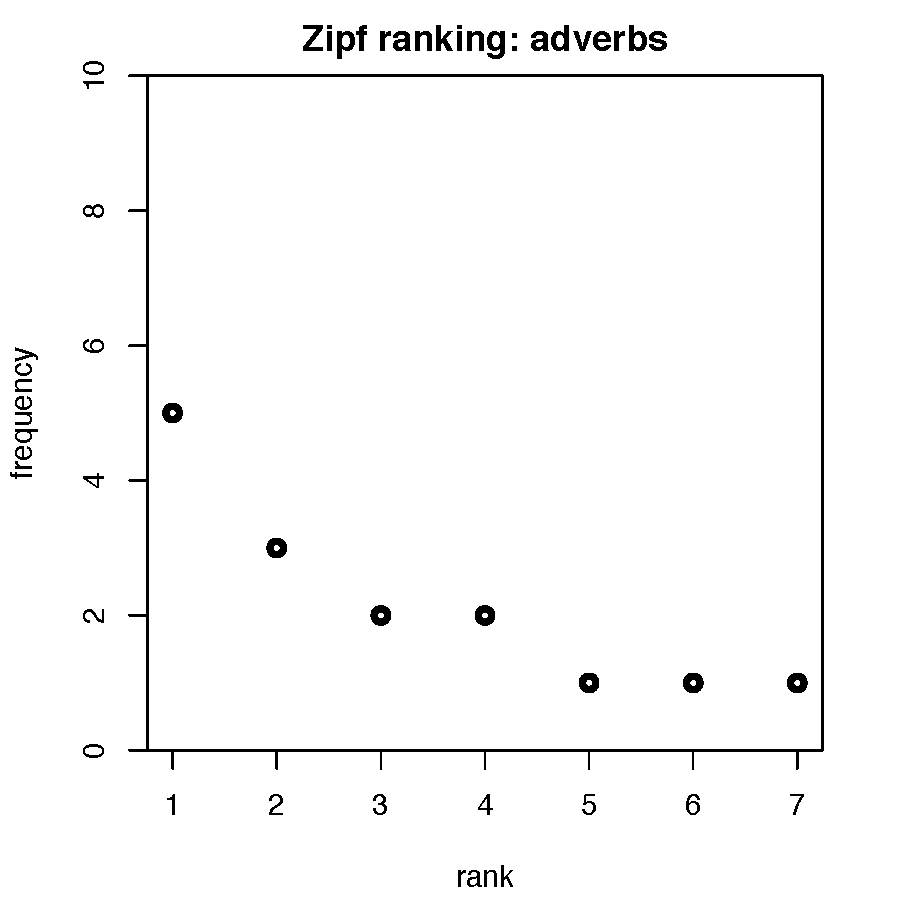
\includegraphics[width=45mm]{../plots/tutorial_tfl}}
    \end{column}
  \end{columns}
\end{frame}

\begin{frame}
  \frametitle{A realistic Zipf ranking: the Brown corpus}

  \gap
  \begin{scriptsize}
    \begin{tabular}{|r|r|l||r|r|l|}
      \hline
      \multicolumn{3}{|c||}{\hh{top frequencies}} & \multicolumn{3}{c|}{\hh{bottom frequencies}}\\
      \hline
      \textbf{\textit{r}} & \multicolumn{1}{c|}{\textbf{\textit{f}}} & \textbf{word} & \textbf{rank range} & \multicolumn{1}{c|}{\textbf{\textit{f}}} & \textbf{randomly selected examples}\\
      \hline
       1 & 69836 & the   &   7731 -- \phantom{0}8271 & 10 &    schedules, polynomials, bleak \\ 
       2 & 36365 & of    &   8272 -- \phantom{0}8922 &  9 &          tolerance, shaved, hymn \\ 
       3 & 28826 & and   &   8923 -- \phantom{0}9703 &  8 & decreased, abolish, irresistible \\ 
       4 & 26126 & to    &   9704 -- 10783 &  7 &        immunity, cruising, titan \\ 
       5 & 23157 & a     &  10784 -- 11985 &  6 &     geographic, lauro, portrayed \\ 
       6 & 21314 & in    &  11986 -- 13690 &  5 &     grigori, slashing, developer \\ 
       7 & 10777 & that  &  13691 -- 15991 &  4 &       sheath, gaulle, ellipsoids \\ 
       8 & 10182 & is    &  15992 -- 19627 &  3 &         mc, initials, abstracted \\ 
       9 &  9968 & was   &  19628 -- 26085 &  2 &         thar, slackening, deluxe \\ 
      10 &  9801 & he    &  26086 -- 45215 &  1 &  beck, encompasses, second-place \\ 
      \hline
    \end{tabular}
  \end{scriptsize}
\end{frame}

\begin{frame}
  \frametitle{A realistic Zipf ranking: the Brown corpus}

  \ungap[1]
  \begin{center}
    \only<beamer:1| handout:0>{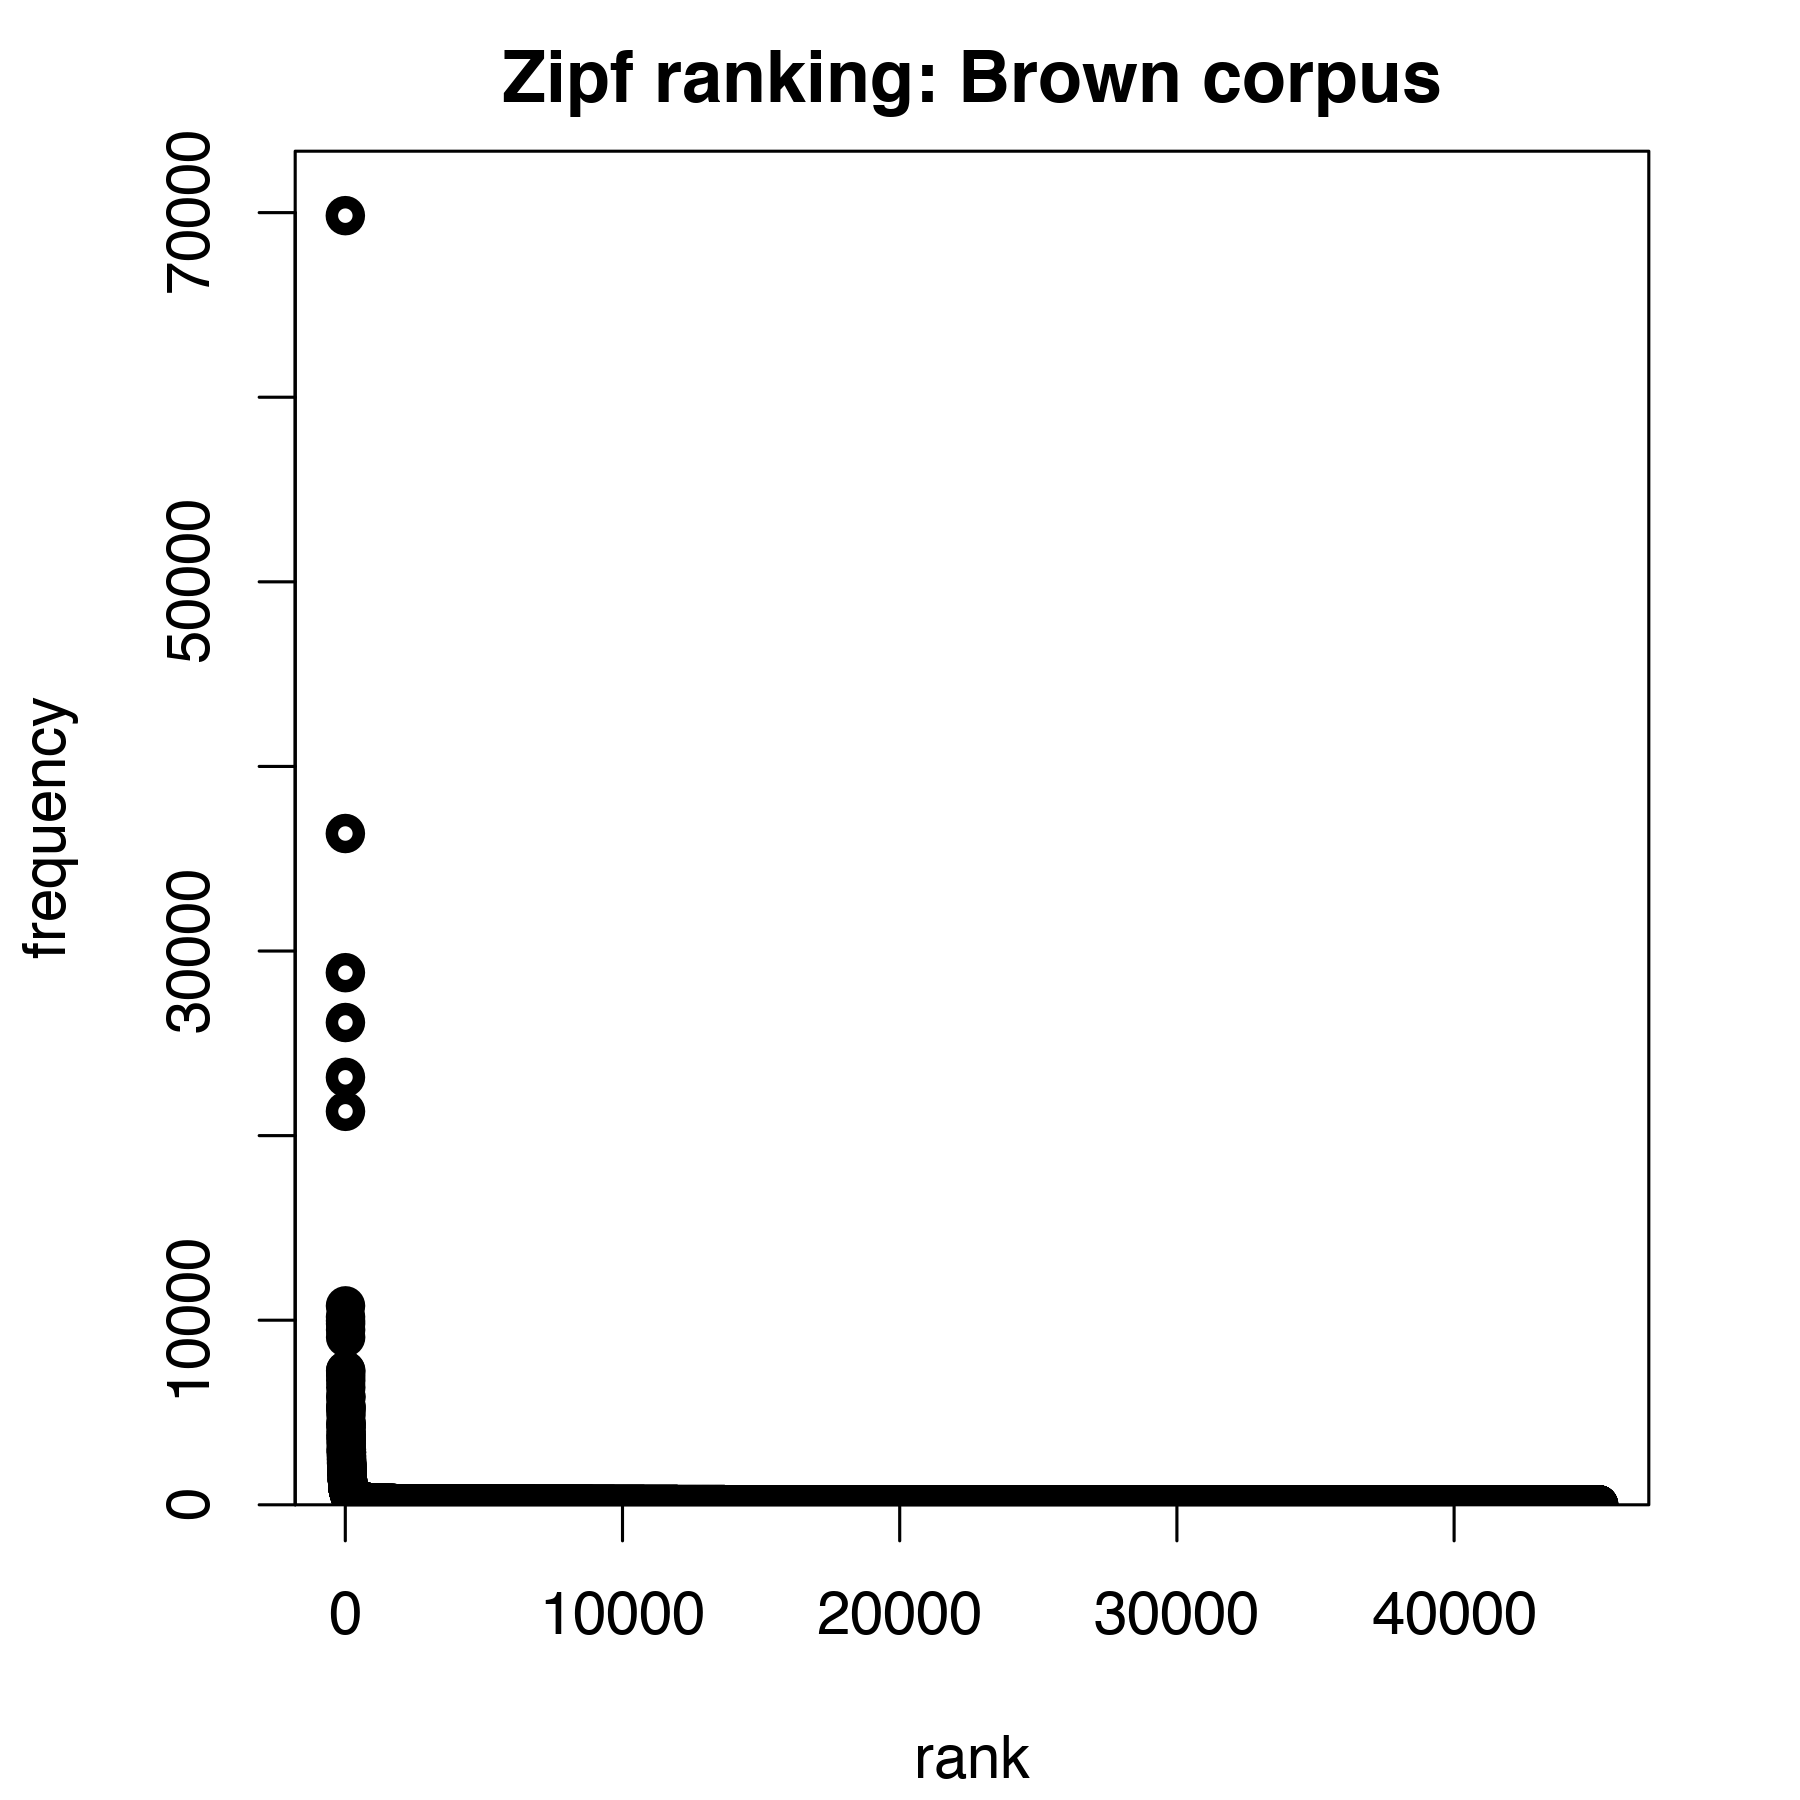
\includegraphics[height=7.5cm]{../plots/tutorial_brown_tfl}}%
    \only<beamer:2| handout:1>{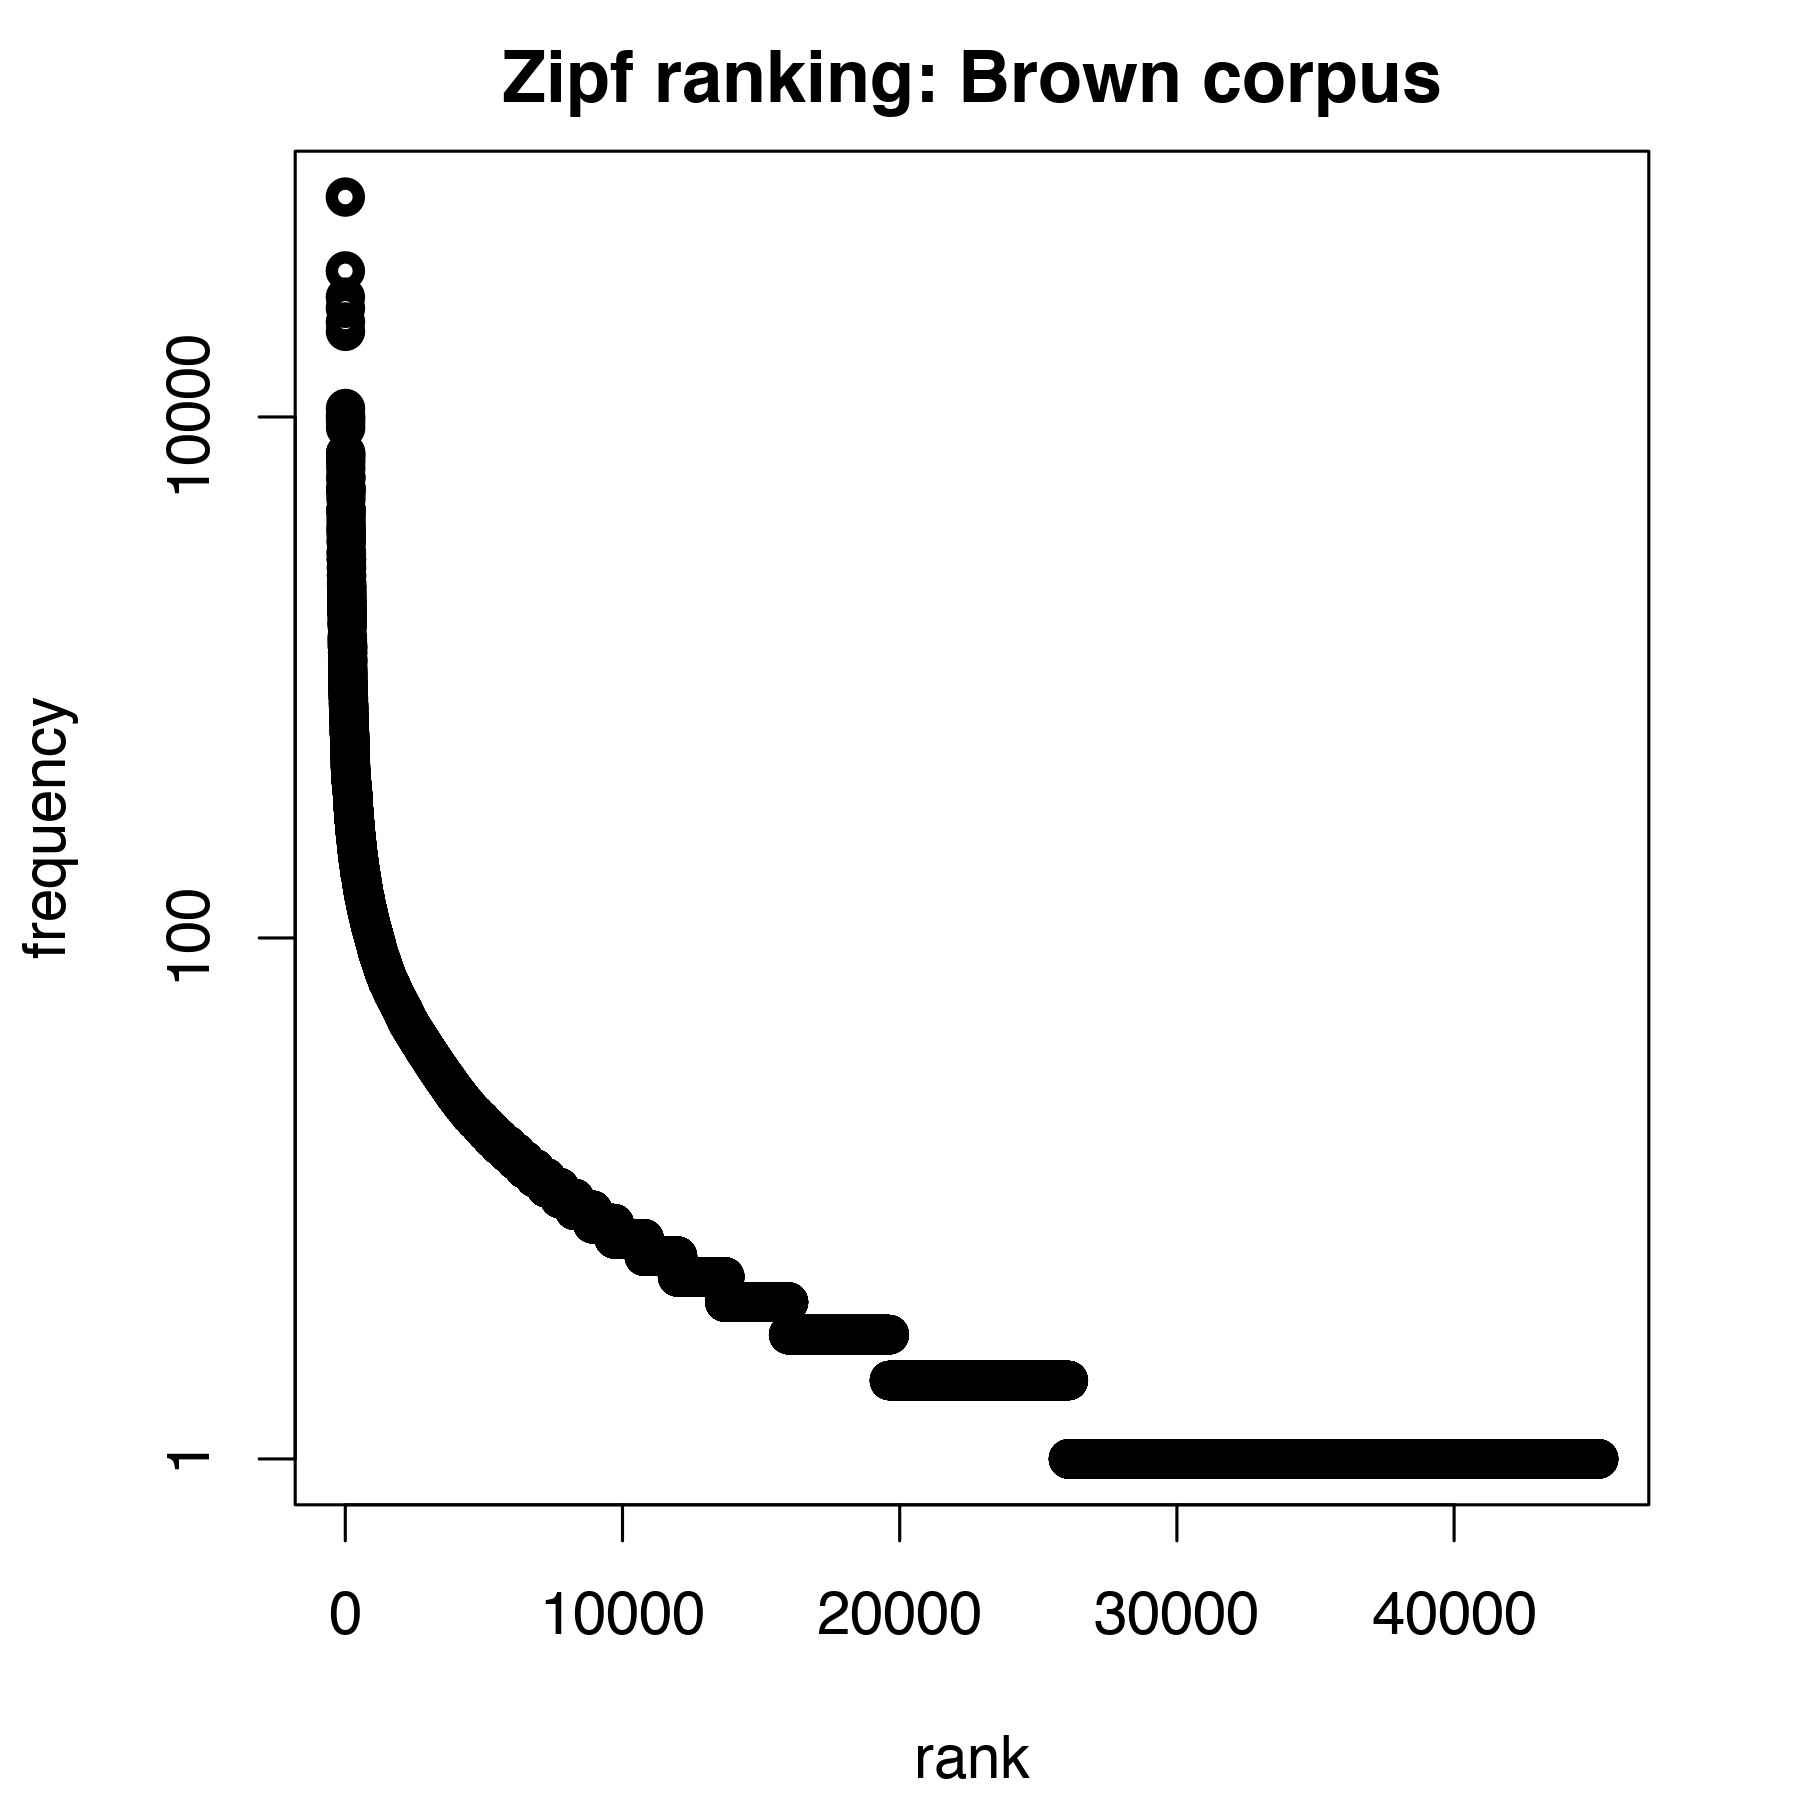
\includegraphics[height=7.5cm]{../plots/tutorial_brown_tfl_log}}%
  \end{center}
\end{frame}

\begin{frame}
  \frametitle{Frequency spectrum}

  \ungap[1.5]
  \begin{itemize}
  \item pool types with $f = 1$ (\primary{hapax legomena}), types with $f = 2$ (\primary{dis legomena}), \ldots, $f = m$, \ldots
  \item $V_1 = 3$: number of hapax legomena (\emph{now, otherwise, recently})
  \item $V_2 = 2$: number of dis legomena (\emph{merely, much})
  \item general definition: $V_m = \abs{\setdef{w}{f_w = m}}$
  \end{itemize}
  
  \begin{columns}[c]
    \begin{column}{35mm}
      \centering
      \textbf{Zipf ranking}

      \begin{tabular}{l|c|c}
        $w$ & $r$ & $f_r$ \\
        \hline
        \TL{very}     & 1 & 5 \\
        \TL{not}      & 2 & 3 \\ 
        \TL{merely}   & 3 & 2 \\ 
        \TL{much}     & 4 & 2 \\ 
        \TL{now}      & 5 & 1 \\
        \TL{otherwise}& 6 & 1 \\ 
        \TL{recently} & 7 & 1 
      \end{tabular}
    \end{column}
    \begin{column}{25mm}
      \centering
      \h{frequency\\ spectrum}

      \begin{tabular}{c|c}
        $m$ & $V_m$ \\
        \hline
        1 & 3 \\
        2 & 2 \\
        3 & 1 \\
        5 & 1
      \end{tabular}
    \end{column}
    \begin{column}{5cm}
      \visible<2->{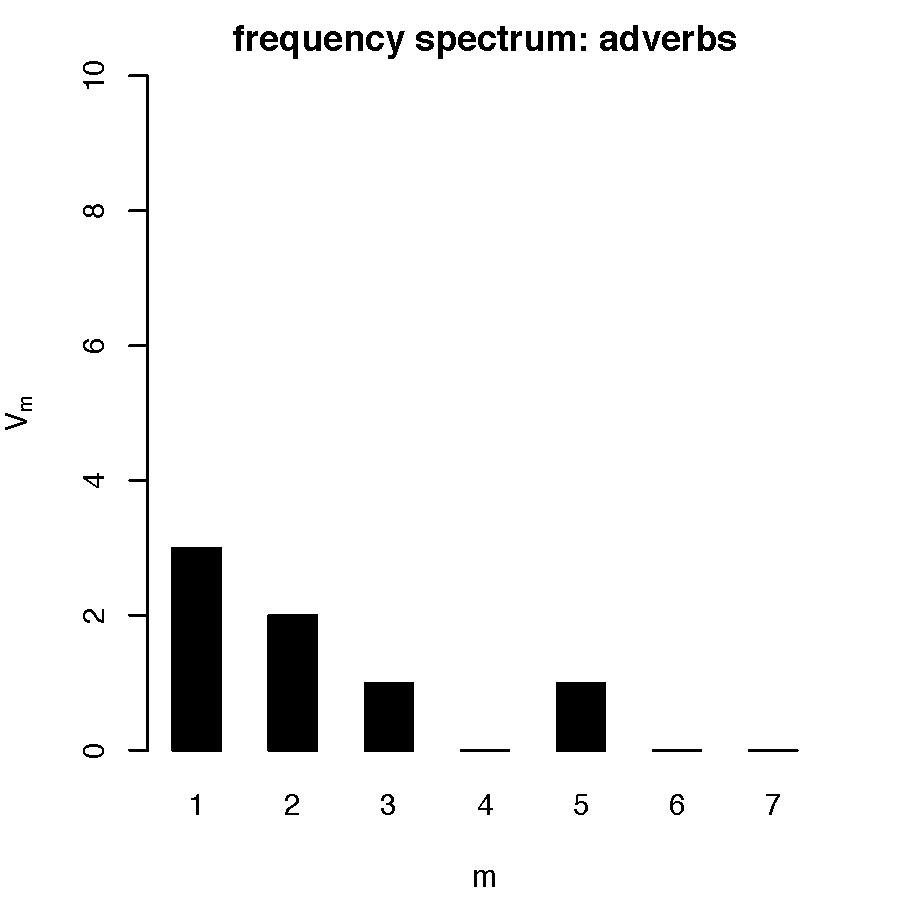
\includegraphics[width=45mm]{../plots/tutorial_spc}}
    \end{column}
  \end{columns}

\end{frame}

\begin{frame}
  \frametitle{A realistic frequency spectrum: the Brown corpus}

  \ungap[1]
  \begin{center}
    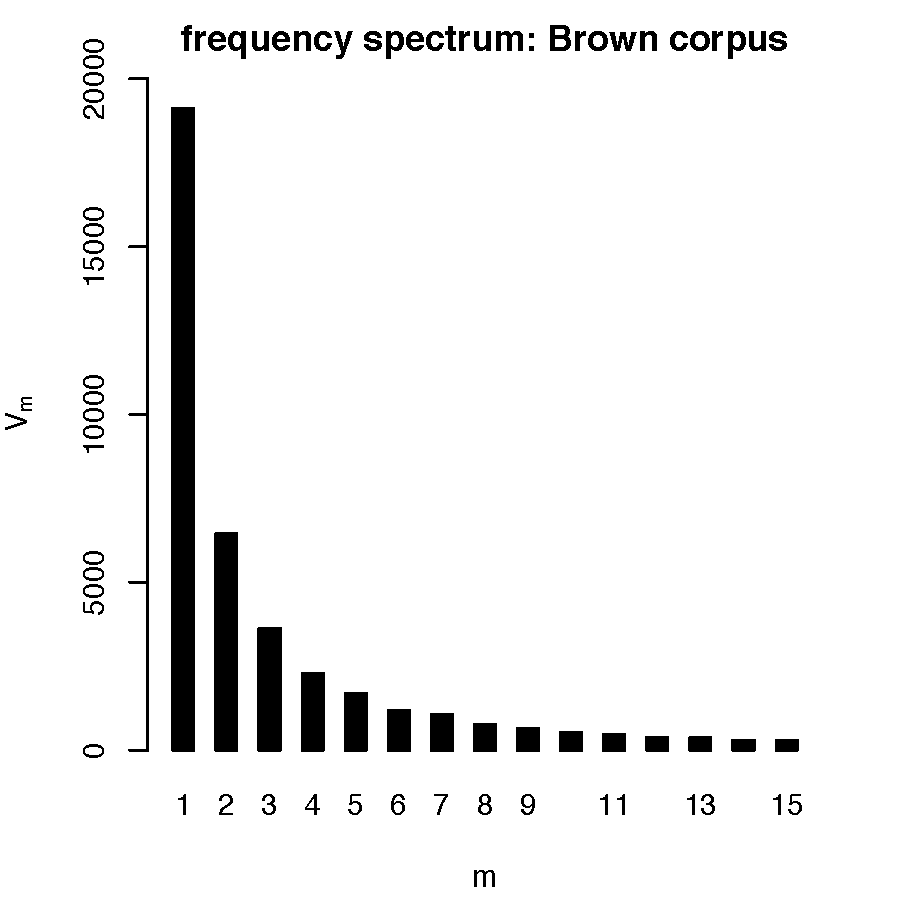
\includegraphics[height=7.5cm]{../plots/tutorial_brown_spc}%
  \end{center}
\end{frame}

\begin{frame}
  \frametitle{Vocabulary growth curve}
  
    our sample: \TA<1->{recently}, \TA<2->{very}, \TA<2->{not}, \TA<3->{otherwise}, \TA<3->{much}, \TA<3->{very},
  \TA<3->{very}, \TA<4->{merely}, \TA<4->{not}, \TA<4->{now}, \TA<4->{very}, \TA<4->{much},
  \TA<5->{merely}, \TA<5->{not}, \TA<5->{very}

  \begin{columns}[c]
    \begin{column}{6cm}
      \begin{itemize}
      \item<1-> $N = 1$, $V(N) = 1$, $V_1(N) = 1$
      \item<2-> $N = 3$, $V(N) = 3$, $V_1(N) = 3$
      \item<3-> $N = 7$, $V(N) = 5$, $V_1(N) = 4$
      \item<4-> $N = 12$, $V(N) = 7$, $V_1(N) = 4$
      \item<5-> $N = 15$, $V(N) = 7$, $V_1(N) = 3$
      \end{itemize}
    \end{column}
    \begin{column}{5cm}
      \visible<6->{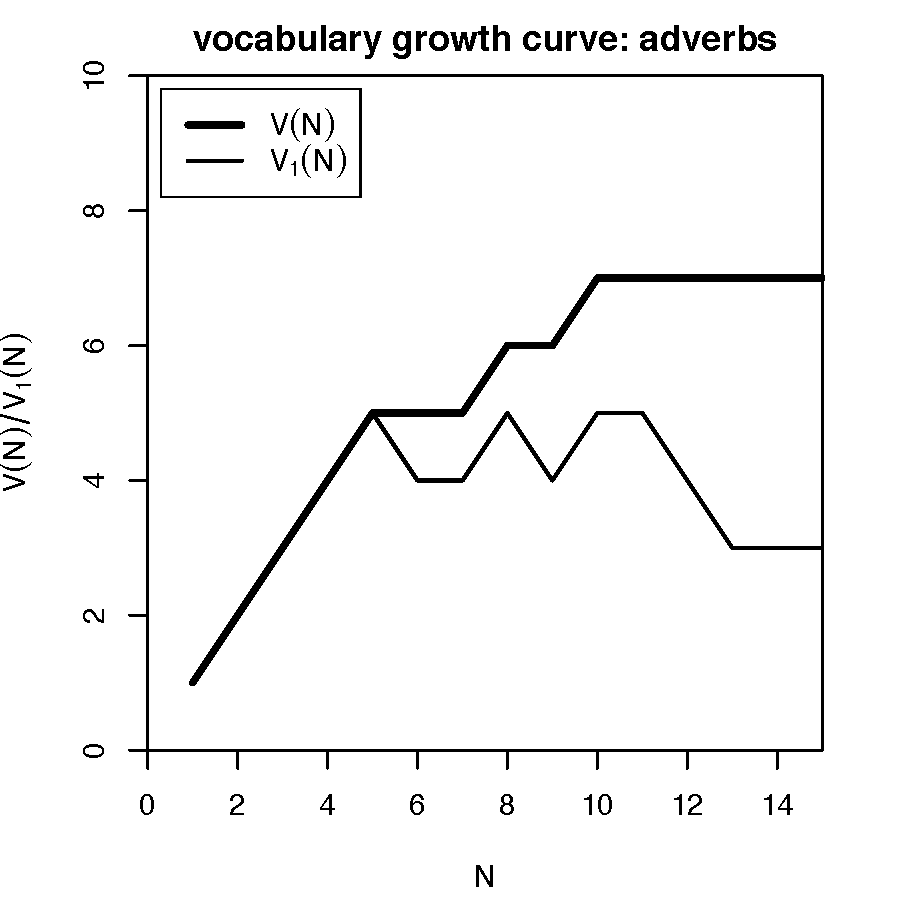
\includegraphics[width=5cm]{../plots/tutorial_vgc}}%
    \end{column}
  \end{columns}

\end{frame}

\begin{frame}
  \frametitle{A realistic vocabulary growth curve: the Brown corpus}

  \ungap[1]
  \begin{center}
    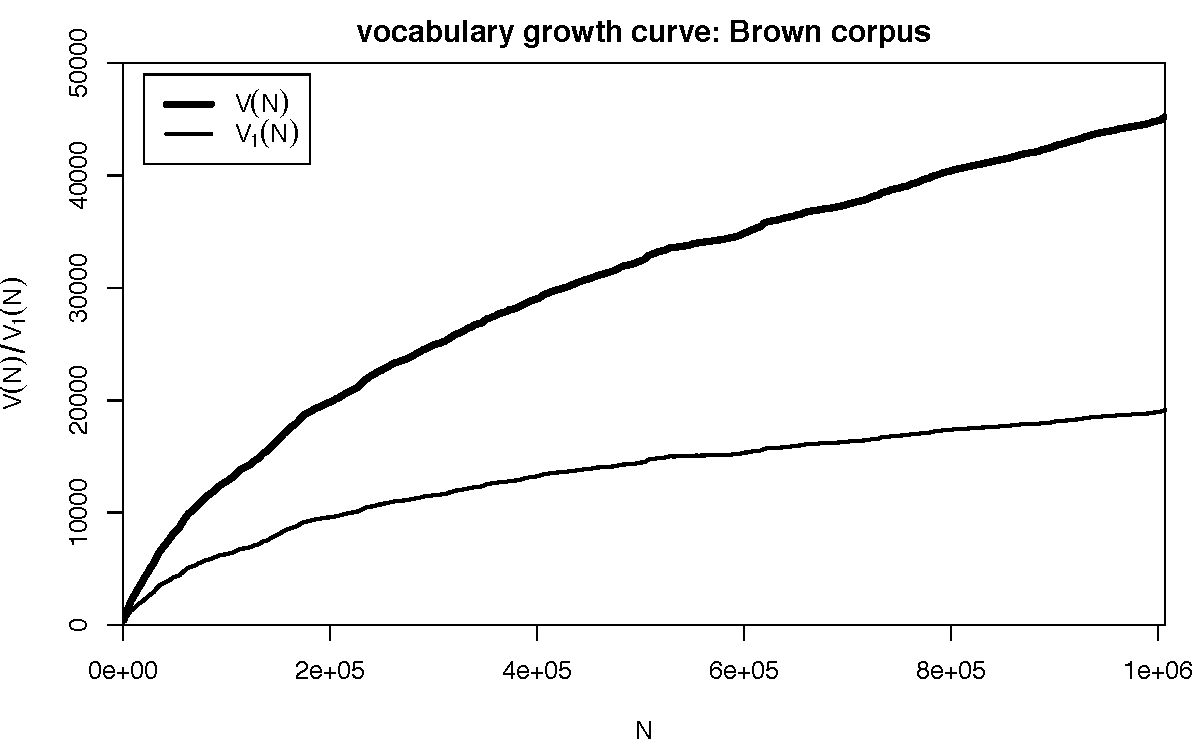
\includegraphics[height=6.5cm]{../plots/tutorial_brown_vgc}%
  \end{center}
\end{frame}

\begin{frame}
  \frametitle{Vocabulary growth in authorship attribution}

  \ungap[1]
  \begin{itemize}
  \item Authorship attribution by n-gram tracing applied to the case of the Bixby letter \citep{Grieve:etc:18}
  \item Word or character n-grams in disputed text are compared against large ``training'' corpora from candidate authors
  \end{itemize}

  \begin{center}
    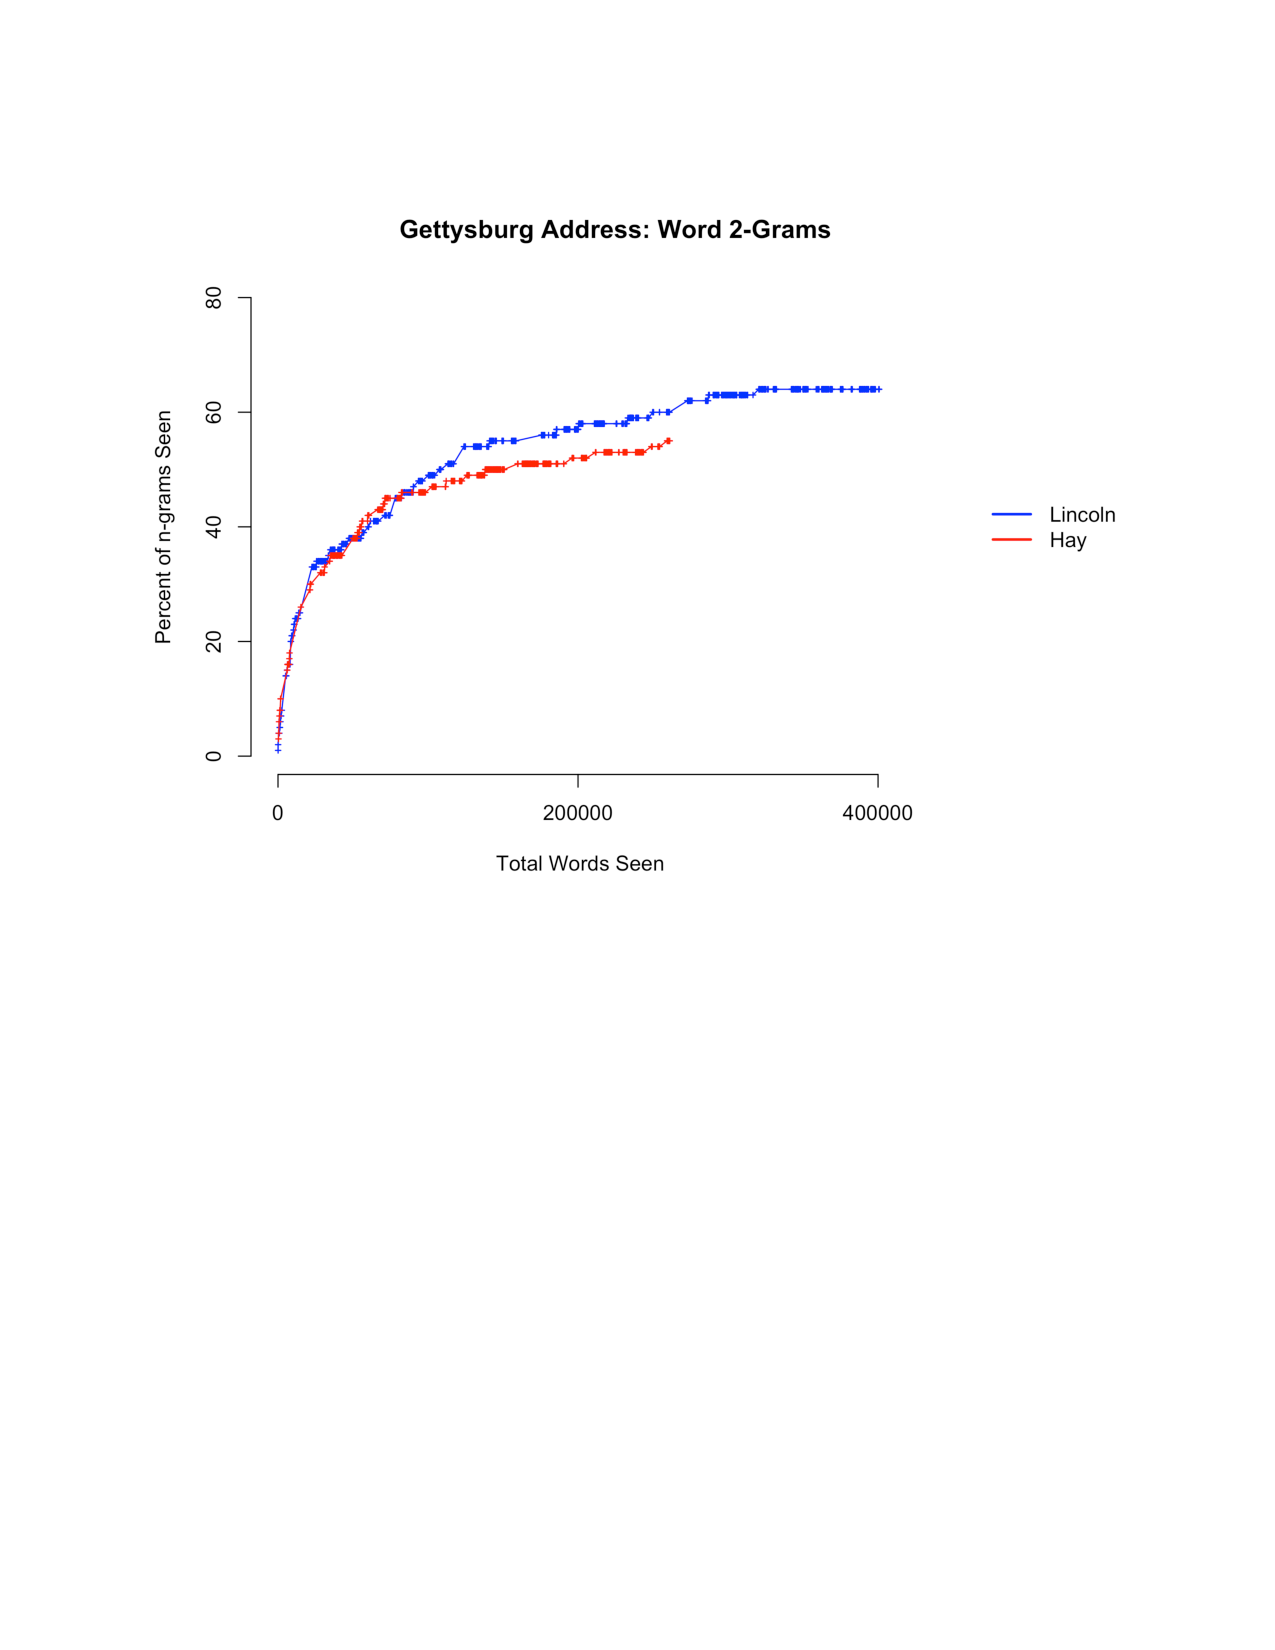
\includegraphics[width=8cm]{img/GrieveEtc2018_fig1}
  \end{center}
\end{frame}

%%%%%%%%%%%%%%%%%%%%%%%%%%%%%%%%%%%%%%%%%%%%%%%%%%%%%%%%%%%%%%%%%%%%%%%%
\subsection{Zipf's law}

\begin{frame}
  \frametitle{Observing Zipf's law}
  \framesubtitle{across languages and different linguistic units}

  \ungap[1.5]
  \begin{center}
    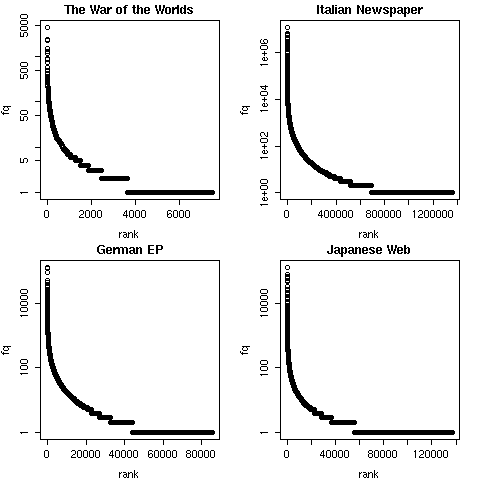
\includegraphics[height=7.5cm]{img/othercorporarf}
  \end{center}
\end{frame}

\begin{frame}<beamer:0| handout:1>
  \frametitle{Observing Zipf's law}
  \framesubtitle{The Italian prefix \TC{ri-} in the \emph{la Repubblica} corpus}

  \begin{center}
    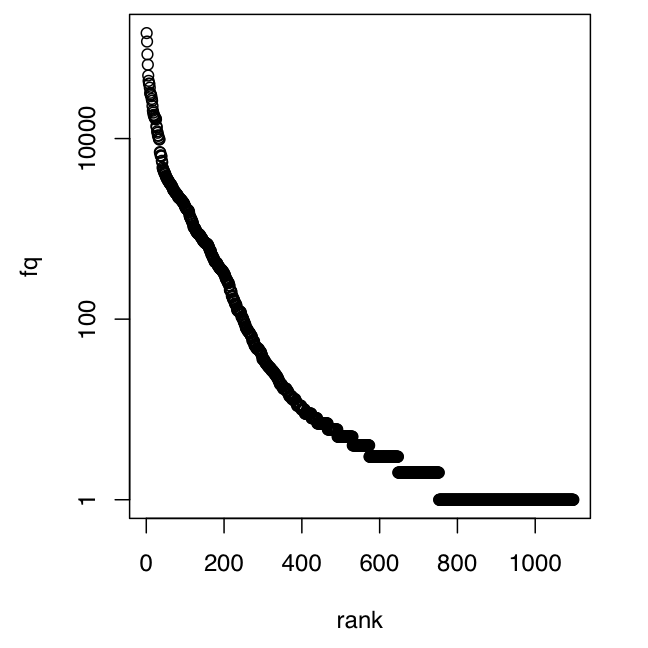
\includegraphics[height=6.5cm]{img/ita-ri-rf}
  \end{center}
\end{frame}

\begin{frame}
  \frametitle{Observing Zipf's law}

  \ungap[1.5]
  \begin{center}
    \only<beamer:1| handout:0>{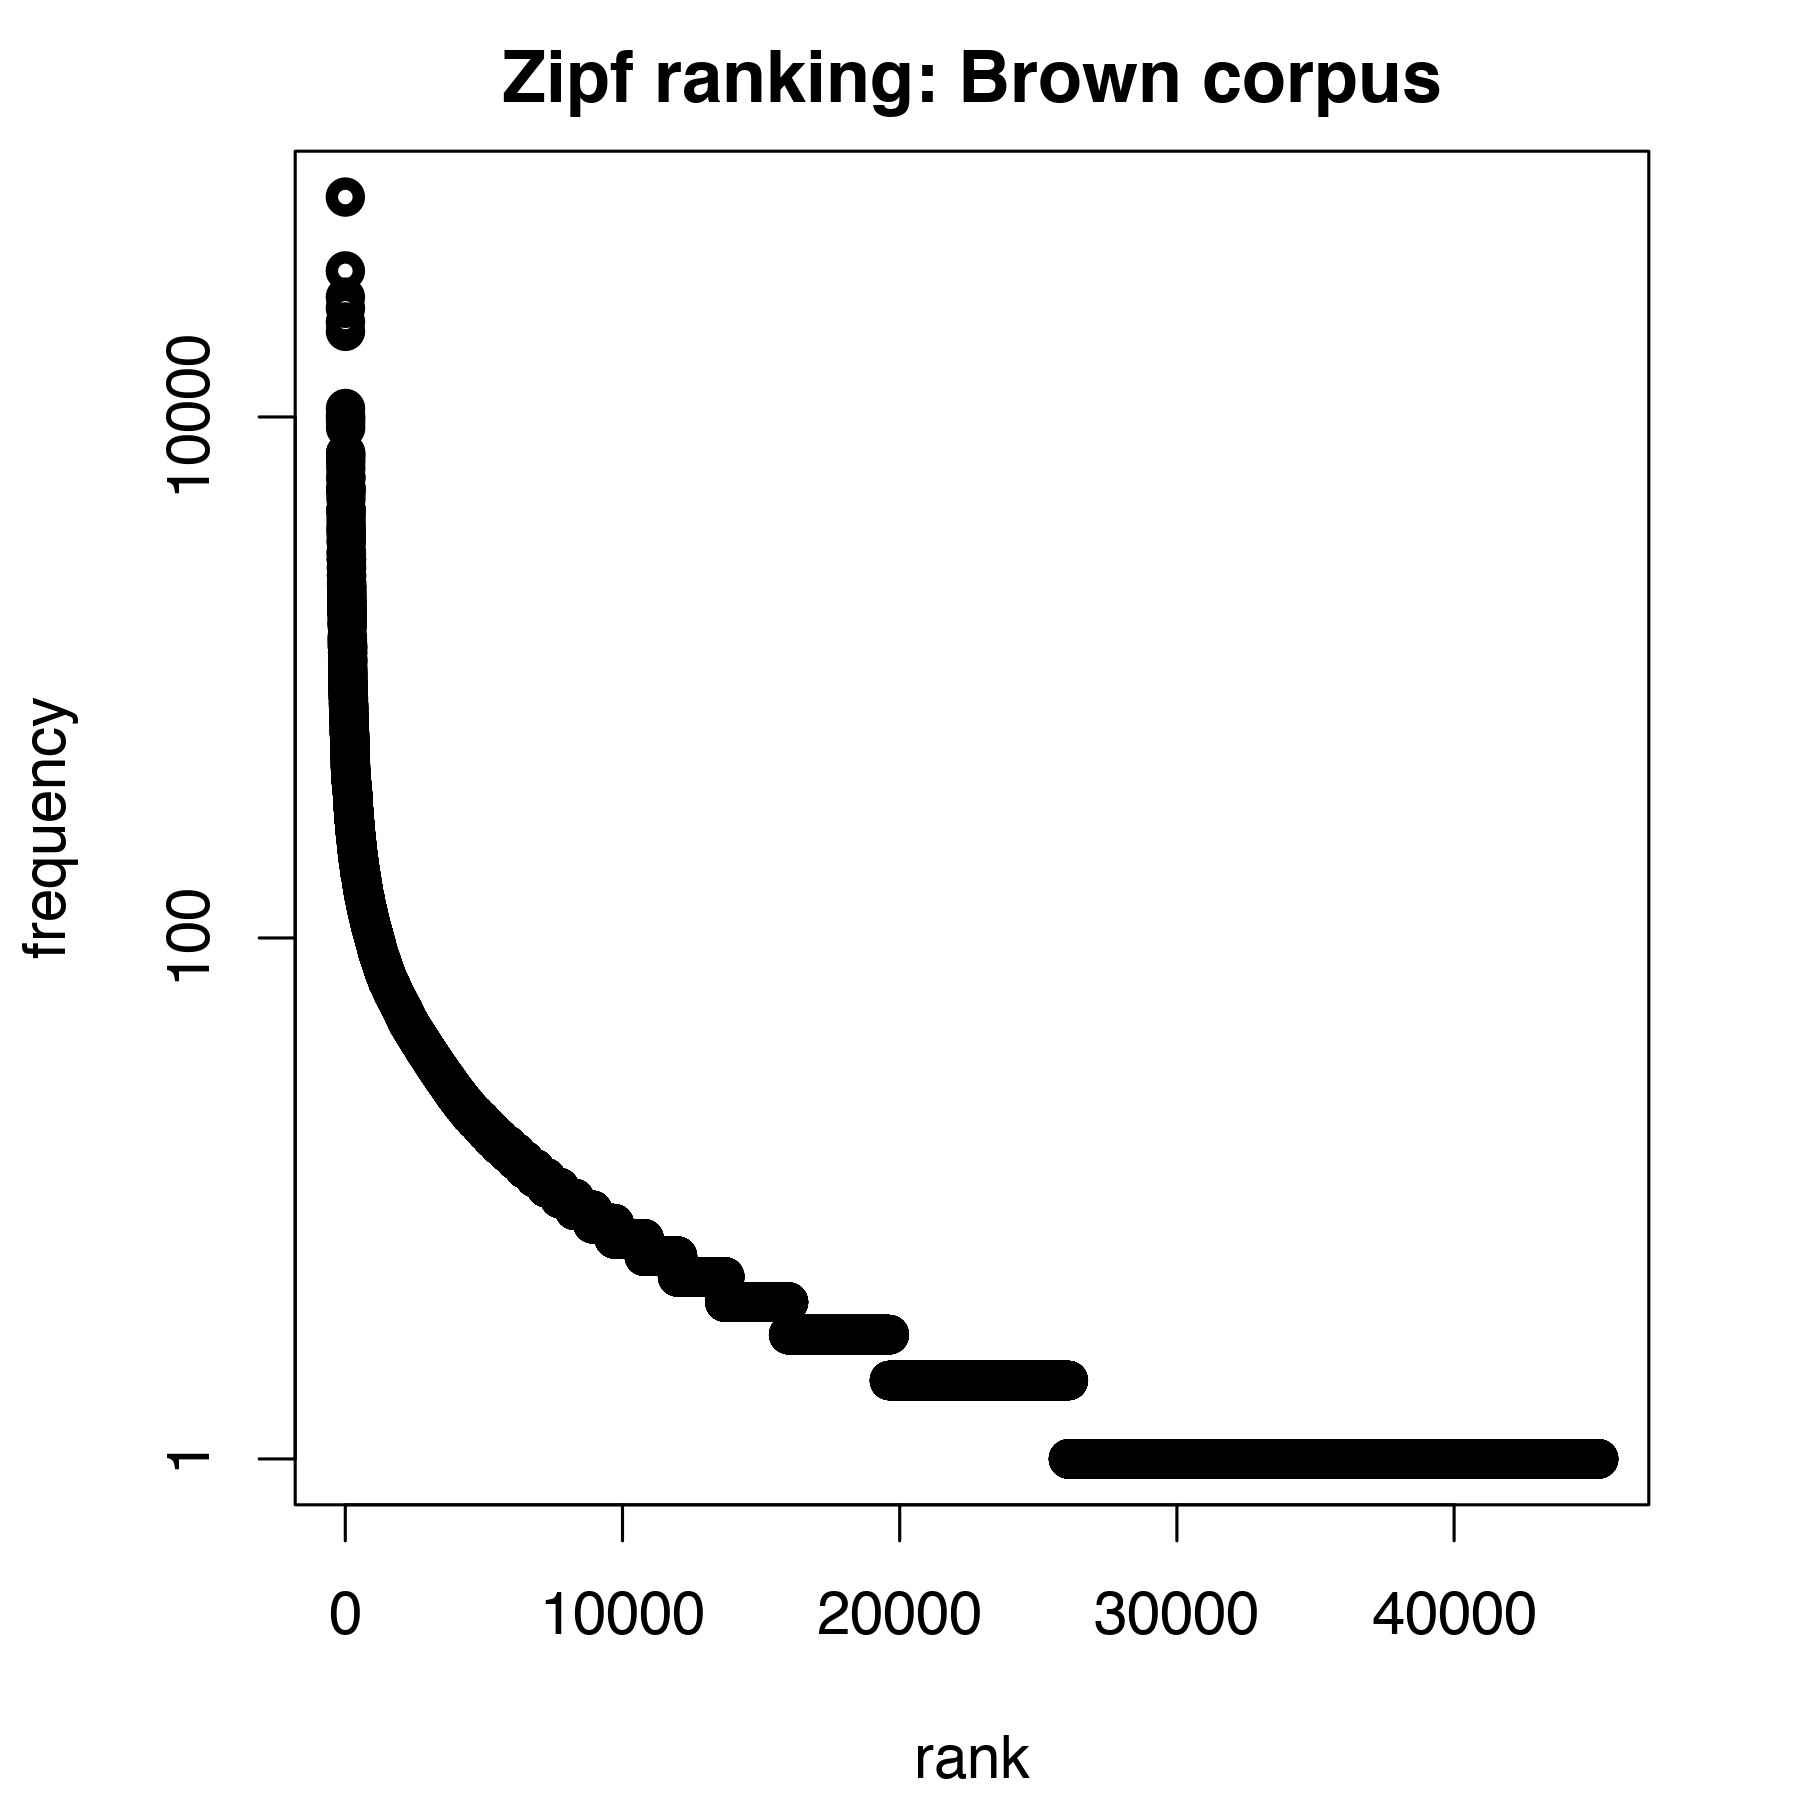
\includegraphics[height=7.5cm]{../plots/tutorial_brown_tfl_log}}%
    \only<beamer:2| handout:1>{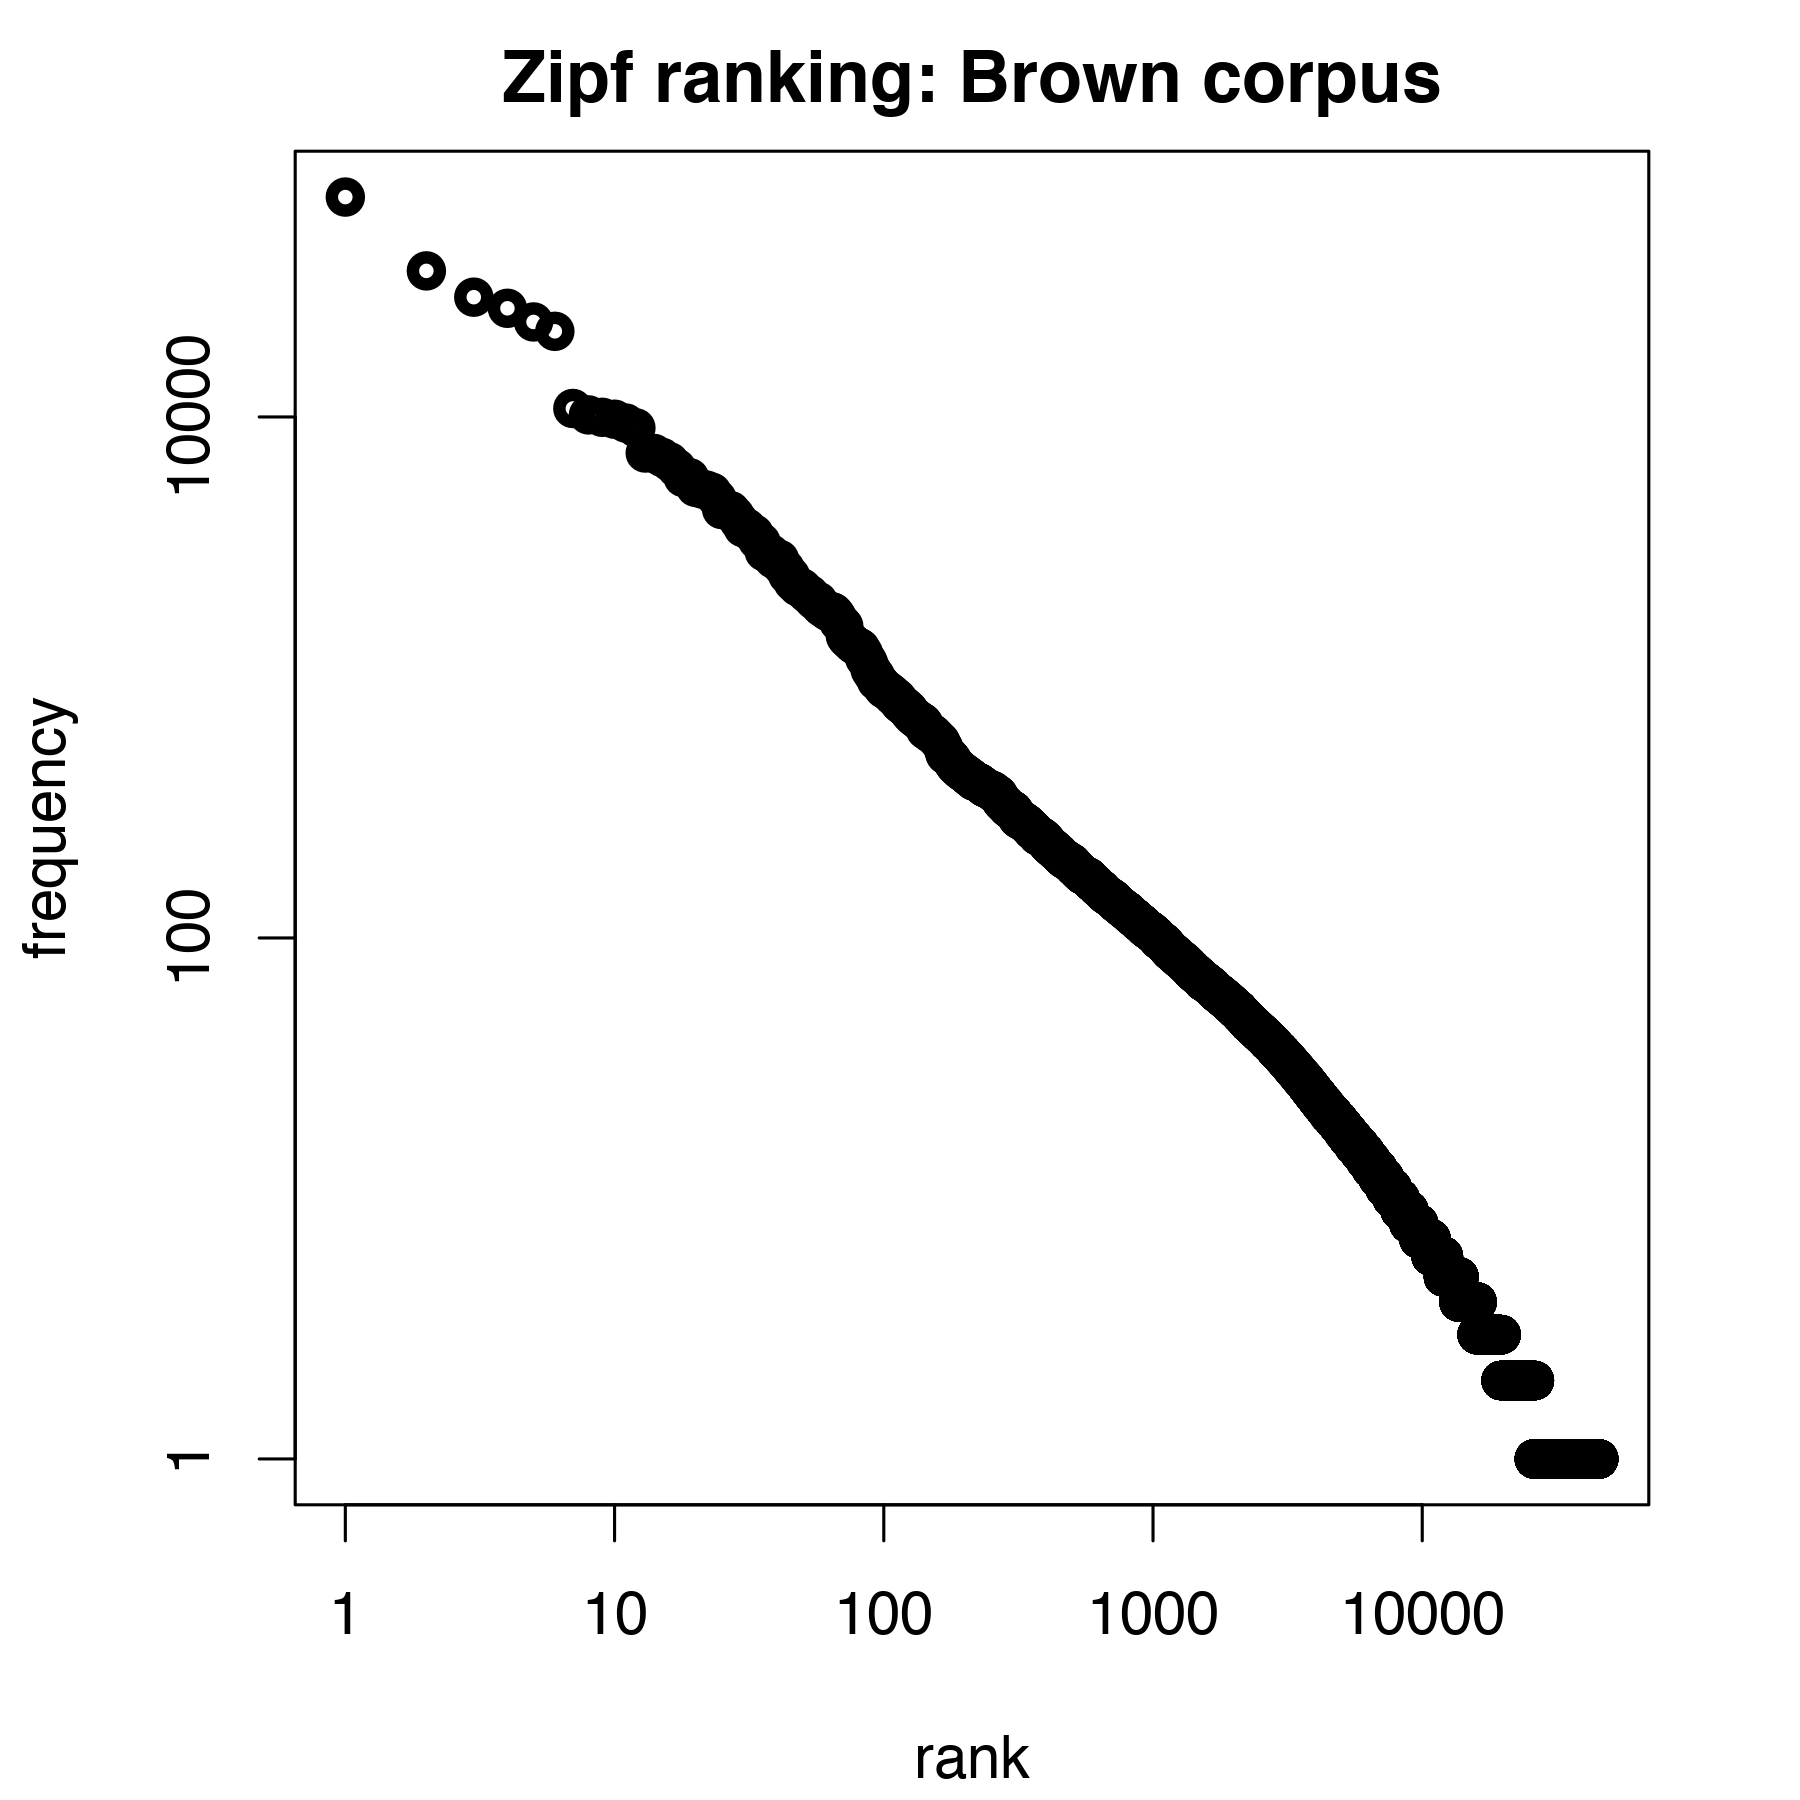
\includegraphics[height=7.5cm]{../plots/tutorial_brown_tfl_loglog}}%
  \end{center}
\end{frame}


\begin{frame}
  \frametitle{Observing Zipf's law}

  \begin{itemize}
  \item Straight line in double-logarithmic space corresponds\\
    to \h{power law} for original variables
  \item This leads to Zipf's (\citeyear{Zipf:49,Zipf:65}) famous law:
    \[
      f_r = \frac{C}{r^a}
    \]
  \item<2-> If we take logarithm on both sides, we obtain:
    \[
    \only<beamer:2| handout:0>{%
      \log f_r = \log C - a \cdot \log r}%
    \only<beamer:3-| handout:1>{%
      \secondary{\underbrace{\log f_r}_y}
      = \log C - a \cdot \secondary{\underbrace{\log r}_x}}%
    \]
  \item<4-> Intuitive interpretation of $a$ and $C$:
    \begin{itemize}
    \item $a$ is \h{slope} determining how fast log frequency decreases
    \item $\log C$ is \h{intercept}, i.e.\ log frequency of most frequent word
      ($r = 1$ \so $\log r = 0$) 
    \end{itemize}
  \end{itemize}

\end{frame}

\begin{frame}
  \frametitle{Observing Zipf's law}
  \framesubtitle{Least-squares fit = linear regression in log-space (Brown corpus)}

  \ungap[1.5]
  \begin{center}
    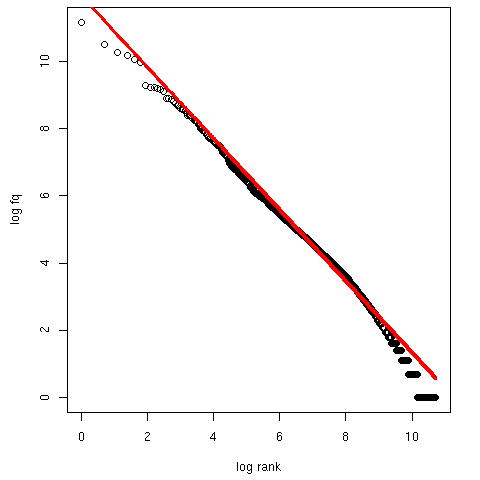
\includegraphics[height=7.5cm]{img/brown-zipf-rf}
  \end{center}
\end{frame}

\begin{frame}
  \frametitle{Zipf-Mandelbrot law}
  \framesubtitle{\citet{Mandelbrot:53,Mandelbrot:62}}

  \begin{itemize}
    \item Mandelbrot's extra parameter:
    \[
    f_r = \frac{C}{(r + b)^a}
    \]
  \item Zipf's law is special case with $b=0$
  \item<2-> Assuming $a=1$, $C=$ 60,000, $b=1$:
    \begin{itemize}
    \item For word with rank 1, Zipf's law predicts frequency of
      60,000; Mandelbrot's variation predicts frequency of 30,000
    \item For word with rank 1,000,  Zipf's law predicts frequency of
      60; Mandelbrot's variation predicts frequency of 59.94
    \item[]
    \end{itemize}
  \item<3-> Zipf-Mandelbrot law forms basis of statistical LNRE models% 
    \begin{itemize}
    \item ZM law derived mathematically as limiting distribution of
      vocabulary generated by a character-level Markov process
    \end{itemize}
  \end{itemize}
\end{frame}

\begin{frame}
  \frametitle{Zipf-Mandelbrot law} 
  \framesubtitle{Non-linear least-squares fit (Brown corpus)}

  \ungap[1.5]
  \begin{center}
    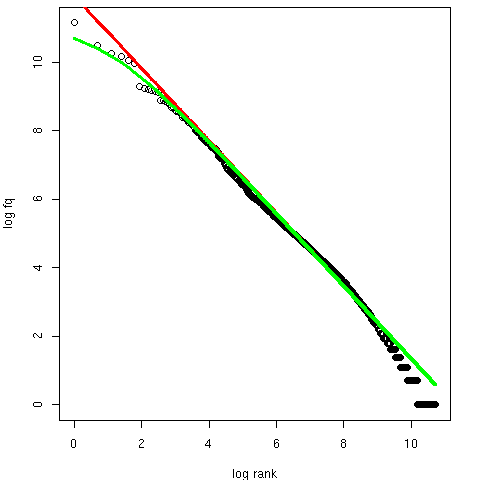
\includegraphics[height=7.5cm]{img/brown-zipf-man-rf}
  \end{center}
\end{frame}


%%%%%%%%%%%%%%%%%%%%%%%%%%%%%%%%%%%%%%%%%%%%%%%%%%%%%%%%%%%%%%%%%%%%%%%%
\subsection{First steps (zipfR)}

\begin{frame}
  \frametitle{zipfR}
  \framesubtitle{\citet{Evert:Baroni:07}}

  \begin{itemize}
  \item \url{http://zipfR.R-Forge.R-Project.org/}
  \item Conveniently available from CRAN repository
  \item Package vignette = gentle tutorial introduction
  \end{itemize}

  \begin{flushright}
    
\includegraphics[width=6cm]{img/zipfR_logo}
    \rule{5mm}{0mm}
  \end{flushright}

\end{frame}

\begin{frame}[fragile]
  \frametitle{First steps with zipfR}

  \begin{itemize}
  \item Set up a folder for this course, and make sure it is your working directory in R (preferably as an RStudio project)
  \item Install the most recent version of the zipfR package
    \begin{itemize}
    \item tutorial requires version 0.7 or newer
    \end{itemize}
  \item Package, handouts, code samples \& data sets available from \url{http://zipfr.r-forge.r-project.org/lrec2018.html}
  \item[]
  \end{itemize}
  
\begin{alltt}
> library(zipfR)

> ?zipfR  \REM{documentation entry point}

> vignette("zipfr-tutorial")  \REM{read the zipfR tutorial}
\end{alltt} 
\end{frame}

\begin{frame}[fragile]
  \frametitle{Loading type-token data}

  \begin{itemize}
  \item Most convenient input: sequence of tokens as text file in vertical format (``one token per line'')
    \begin{itemize}
    \item[\hand] mapped to appropriate types: normalized word forms, word pairs, lemmatized, semantic class, n-gram of POS tags, \ldots
    \item[\hand] language data should always be in UTF-8 encoding!
    \item[\hand] large files can be compressed (\texttt{.gz}, \texttt{.bz2}, \texttt{.xz})
    \item[]
    \end{itemize}
  \item<2-> Sample data: \verb|brown_adverbs.txt| on tutorial homepage
    \begin{itemize}
    \item lowercased adverb tokens from Brown corpus (original order)
    \item[\hand] download and save to your working directory
    \end{itemize}
  \end{itemize}

  \onslide<3->
\begin{alltt}
> adv <- readLines("brown_adverbs.txt", encoding="UTF-8")

> head(adv, 30) \REM{mathematically, a ``vector'' of tokens}
> length(adv)   \REM{sample size = 52,037 tokens}
\end{alltt}
\end{frame}

\begin{frame}[fragile]
  \frametitle{Descriptive statistics: type-frequency list}

  \ungap[1]
\begin{alltt}
> adv.tfl <- vec2tfl(adv)
> adv.tfl \begin{Rout}
       k    f  type
not    1 4859   not
n't    2 2084   n't
so     3 1464    so
only   4 1381  only
then   5 1374  then
now    6 1309   now
even   7 1134  even
as     8 1089    as
       \(\vdots\)    \(\vdots\)     \(\vdots\)
     N    V
 52037 1907
\end{Rout}
> N(adv.tfl)  \REM{sample size}
> V(adv.tfl)  \REM{type count}
\end{alltt}
\end{frame}

\begin{frame}[fragile]
  \frametitle{Descriptive statistics: type-frequency list}

  \begin{itemize}
  \item Visualize descriptive statistics with \texttt{plot} method
  \end{itemize}

\begin{alltt}
> plot(adv.tfl)              \REM{Zipf ranking}
> plot(adv.tfl, log="xy")    \REM{logarithmic scale recommended}
\end{alltt}

  \begin{center}
    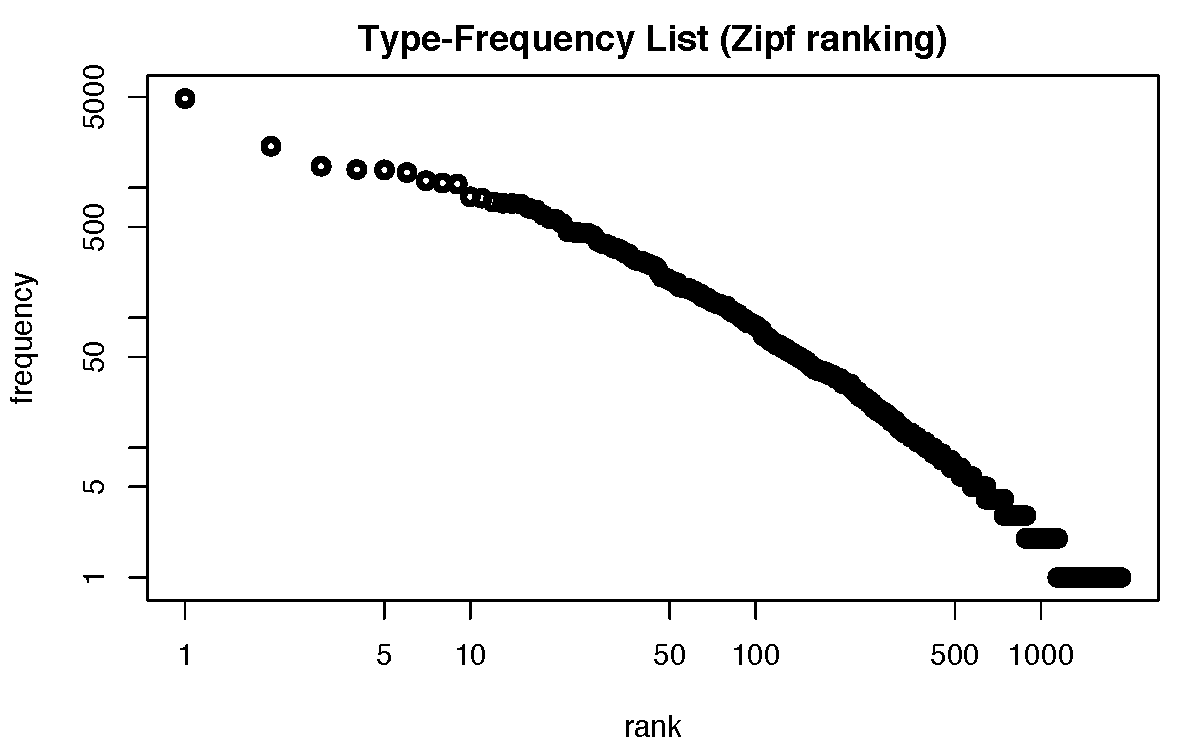
\includegraphics[width=9cm]{img/brown_adverbs_tfl}
  \end{center}
\end{frame}

\begin{frame}[fragile]
  \frametitle{Descriptive statistics: frequency spectrum}

  \ungap[1]
\begin{alltt}
> adv.spc <- tfl2spc(adv.tfl)  \REM{or directly with \texttt{vec2spc}}
> adv.spc \begin{Rout}
    m  Vm
1   1 762
2   2 260
3   3 144
4   4  99
5   5  69
6   6  50
7   7  40
8   8  34
    \(\vdots\)   \(\vdots\)
     N    V
 52037 1907
\end{Rout}
> N(adv.spc)  \REM{sample size}
> V(adv.spc)  \REM{type count}
\end{alltt}
\end{frame}

\begin{frame}[fragile]
  \frametitle{Descriptive statistics: frequency spectrum}

\begin{alltt}
> plot(adv.spc)      \REM{barplot of frequency spectrum}
> ?plot.spc          \REM{see help page for further options}
\end{alltt}

  \begin{center}
    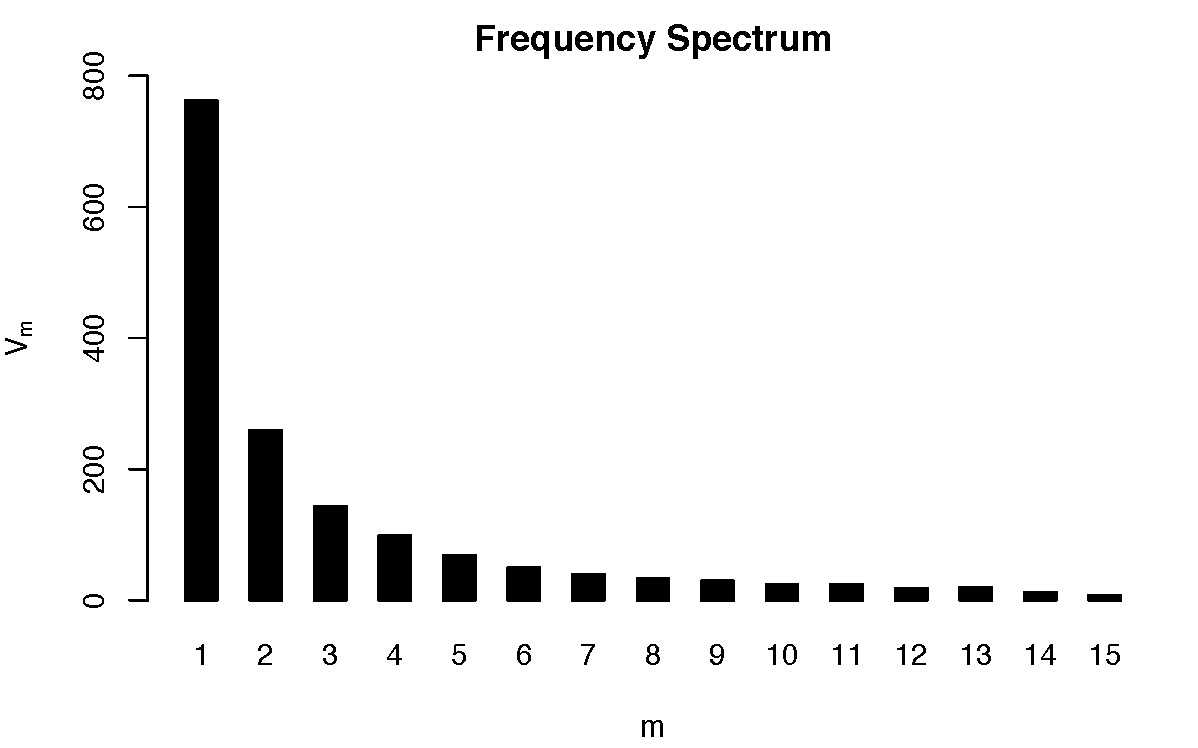
\includegraphics[width=9cm]{img/brown_adverbs_spc}
  \end{center}
\end{frame}

\begin{frame}[fragile]
  \frametitle{Descriptive statistics: vocabulary growth}

  \begin{itemize}
  \item VGC lists vocabulary size $V(N)$ at different sample sizes $N$
  \item Optionally also spectrum elements $V_m(N)$ up to \texttt{m.max}
  \end{itemize}
  
\begin{alltt}
> adv.vgc <- vec2vgc(adv, m.max=2) 
> plot(adv.vgc, add.m=1:2) \REM{plot all three VGCs}
\end{alltt}

  \begin{center}
    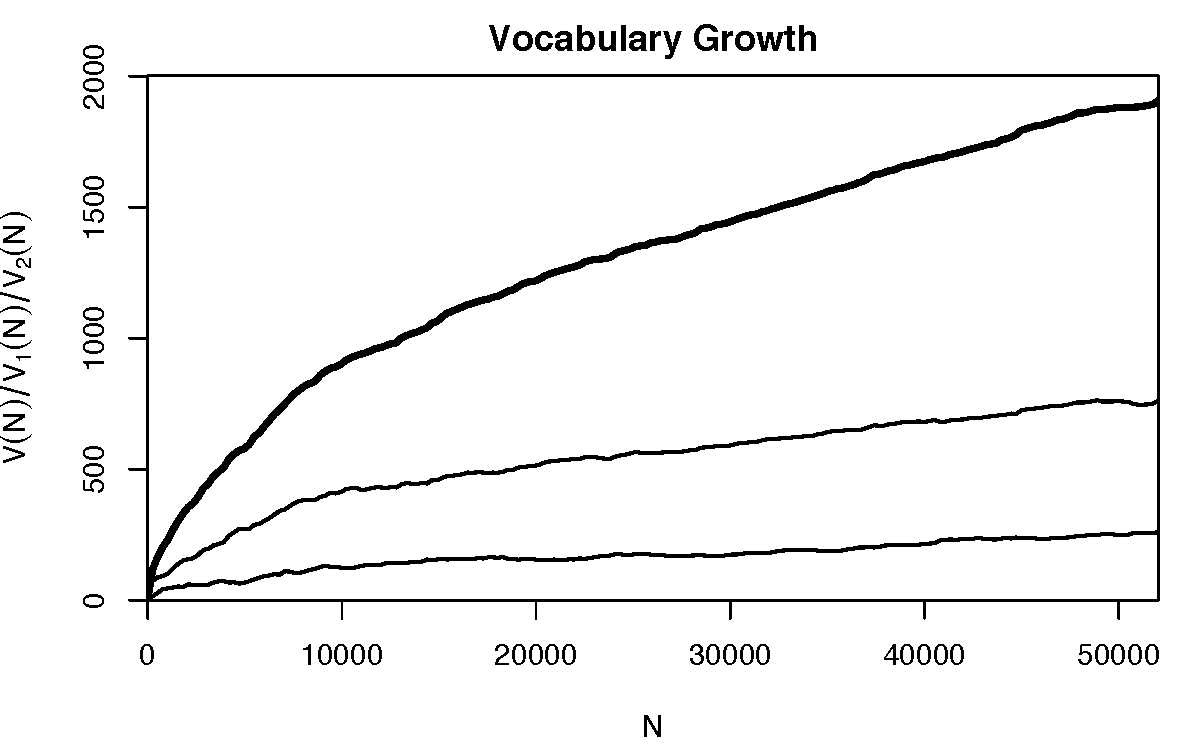
\includegraphics[width=9cm]{img/brown_adverbs_vgc}
  \end{center}
\end{frame}

\begin{frame}[fragile]
  \frametitle{Further example data sets}

  \begin{description}[labelwidth=5cm]
  \item[\texttt{?Brown}] words from Brown corpus
  \item[\texttt{?BrownSubsets}] various subsets
  \item[\texttt{?Dickens}] words from novels by Charles Dickens
  \item[\texttt{?ItaPref}] Italian word-formation prefixes
  \item[\texttt{?TigerNP}] NP and PP patterns from German Tiger treebank
  \item[\texttt{?Baayen2001}] frequency spectra from \citet{Baayen:01}
  \item[\texttt{?EvertLuedeling2001}] German word-formation affixes \citep[manually corrected data from][]{Evert:Luedeling:01}
  \end{description}

  \h{Practice:}
  \begin{itemize}
  \item Explore these data sets with descriptive statistics
  \item Try different plot options (from help pages \texttt{?plot.tfl}, \texttt{?plot.spc}, \texttt{?plot.vgc})
  \end{itemize}
\end{frame}


%%%%%%%%%%%%%%%%%%%%%%%%%%%%%%%%%%%%%%%%%%%%%%%%%%%%%%%%%%%%%%%%%%%%%%%%
%%%%%%%%%%%%%%%%%%%%%%%%%%%%%%%%%%%%%%%%%%%%%%%%%%%%%%%%%%%%%%%%%%%%%%%%
\section{LNRE models}

%%%%%%%%%%%%%%%%%%%%%%%%%%%%%%%%%%%%%%%%%%%%%%%%%%%%%%%%%%%%%%%%%%%%%%%%
\subsection{Population \& samples}

\begin{frame}
  \frametitle{Why do we need statistics?}

  \begin{itemize}
  \item Often want to compare samples of different sizes
    \begin{itemize}
    \item[\hand] extrapolation of VGC \& productivity measures
    \item[]
    \end{itemize}
  \item<2-> Interested in productivity of affix, vocabulary of author, \ldots; not in a particular text or sample\\
    \begin{itemize}
    \item[\hand] statistical inference from sample to population
    \item[\hand] significance of differences in productivity
    \item[]
    \end{itemize}
  \item<3-> Discrete frequency counts are difficult to capture with generalizations such as Zipf's law
    \begin{itemize}
    \item[\hand] Zipf's law predicts many impossible types with $1 < f_r < 2$
    \item[\hand] population does not suffer from such quantization effects
    \end{itemize}
  \end{itemize}
\end{frame}

\begin{frame}
  \frametitle{LNRE models}

  \begin{itemize}
  \item This tutorial introduces the state-of-the-art LNRE approach proposed by \citet{Baayen:01}
    \begin{itemize}
    \item LNRE = Large Number of Rare Events
    \item[]
    \end{itemize}
  \item LNRE uses various approximations and simplifications to obtain a tractable and elegant model
    \begin{itemize}
    \item[]
    \end{itemize}
  \item Of course, we could also estimate the precise discrete distributions using MCMC simulations, but \ldots
    \begin{enumerate}
    \item LNRE model usually minor component of complex procedure
    \item often applied to very large samples ($N > 1$ M tokens)
    \item still better than naive least-squares regression on Zipf ranking
    \end{enumerate}
  \end{itemize}
\end{frame}

\begin{frame}
  \frametitle{The LNRE population}

  \begin{itemize}
  \item Population: set of $S$ types $w_i$ with occurrence \h{probabilities} $\pi_i$
  \item $S$ = \h{population diversity} can be finite or infinite ($S = \infty$)
  \item Not interested in specific types \so  arrange by decreasing
    probability: $\pi_1\geq \pi_2\geq \pi_3 \geq \cdots$
    \begin{itemize}
    \item[\hand] impossible to determine probabilities of all individual types
    \end{itemize}
  \item Normalization: $\pi_1 + \pi_2 + \ldots + \pi_S = 1$
    \begin{itemize}
    \item[]
    \end{itemize}
  \item<2-> Need \hh{parametric} statistical \hh{model} to describe full population (esp.\ for $S = \infty$),
    i.e.\ a function $i \mapsto \pi_i$
    \begin{itemize}
    \item type probabilities $\pi_i$ cannot be estimated reliably from a sample, but parameters of this function can
    \item NB: population index $i$ $\neq$ Zipf rank $r$
    \end{itemize}
  \end{itemize}
\end{frame}

\begin{frame}
  \frametitle{What should the population look like?}
  
  \ungap[1.5]
  \begin{center}
    \begin{tabular}{cc}
      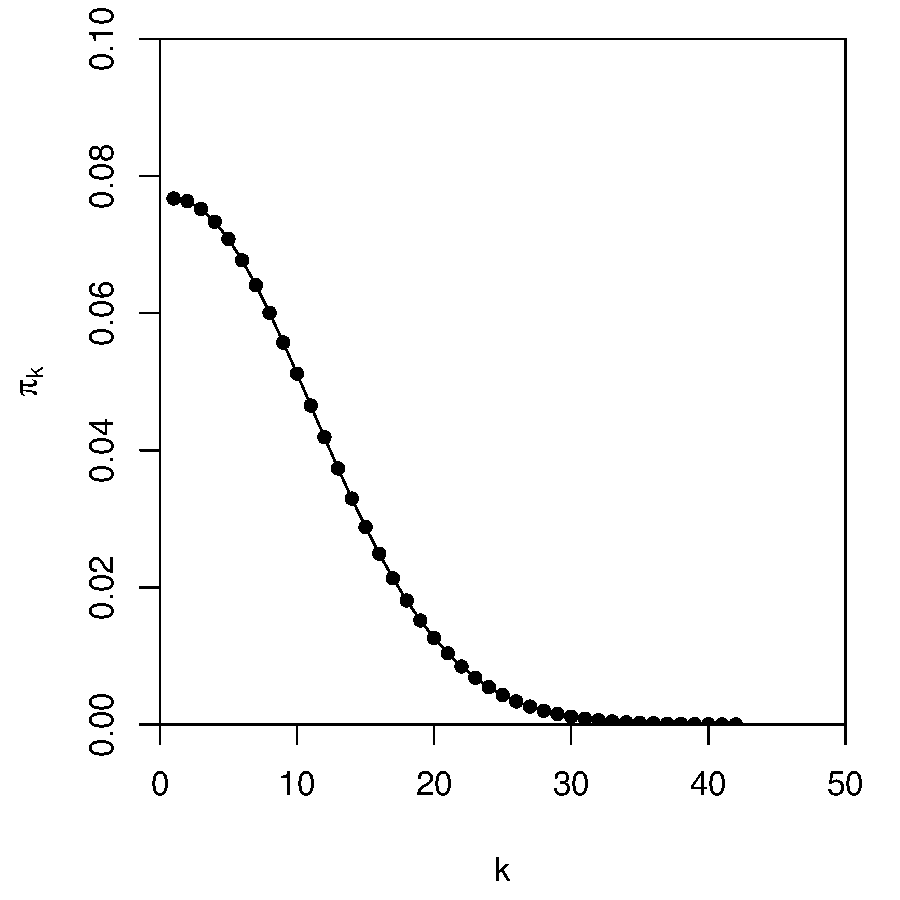
\includegraphics[width=40mm]{img/05-models-normal} &
      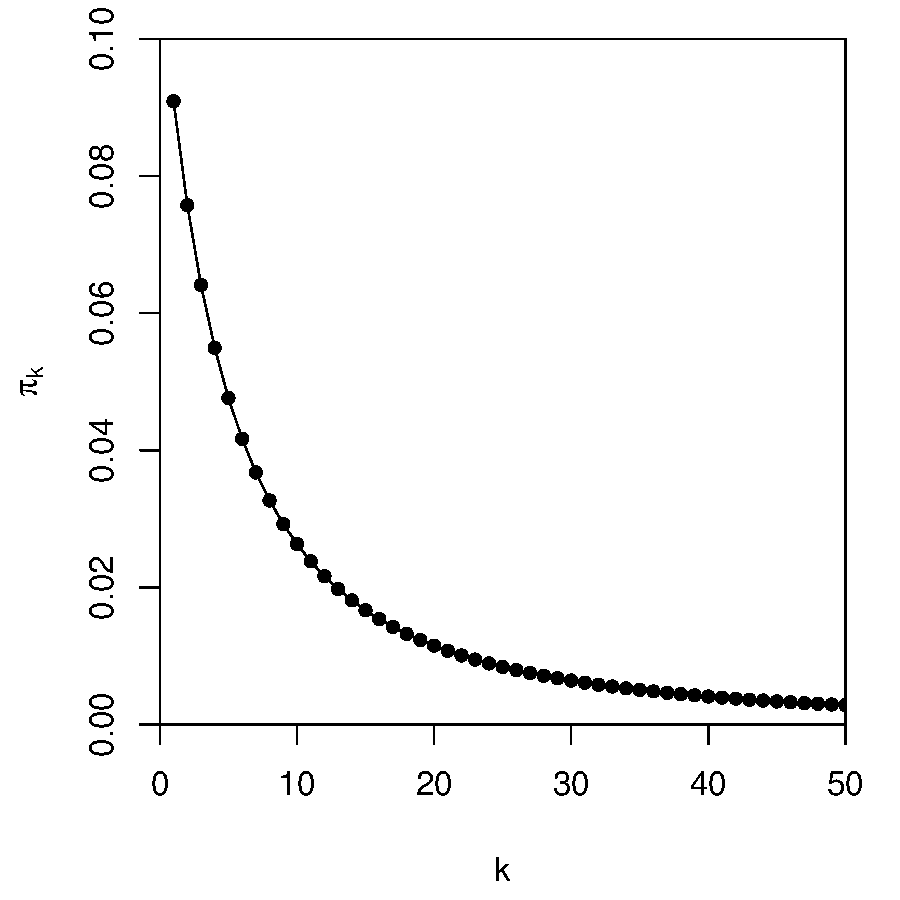
\includegraphics[width=40mm]{img/05-models-zm-1} \\
      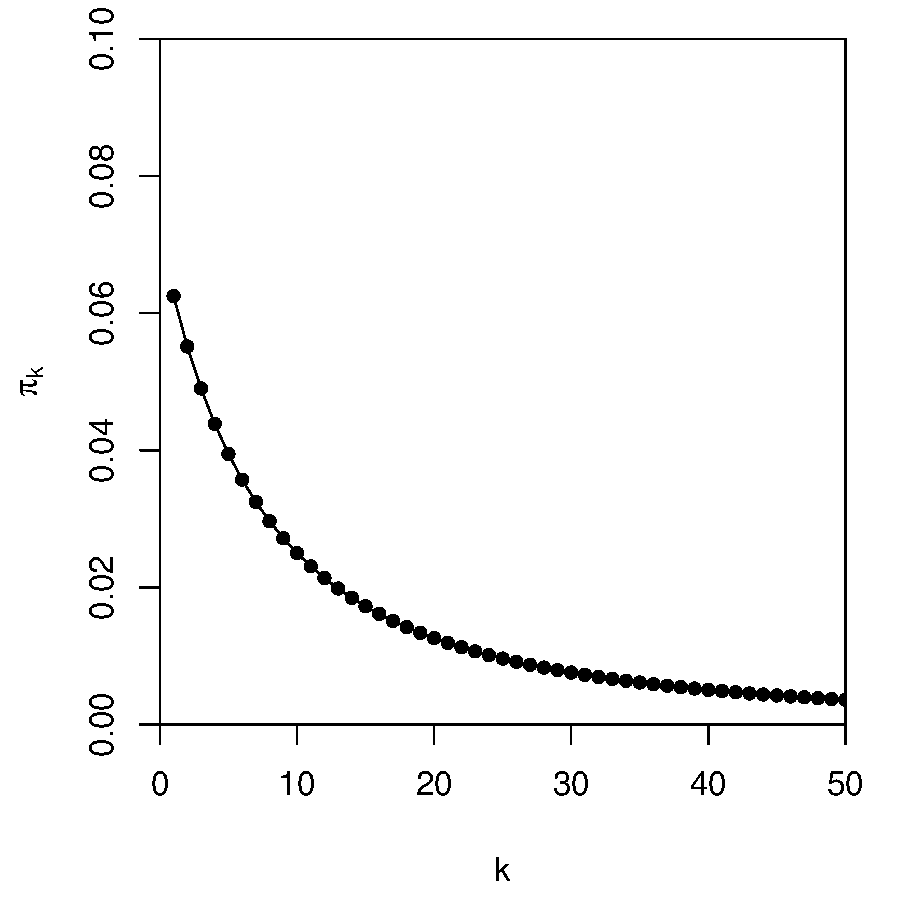
\includegraphics[width=40mm]{img/05-models-zm-3} &
      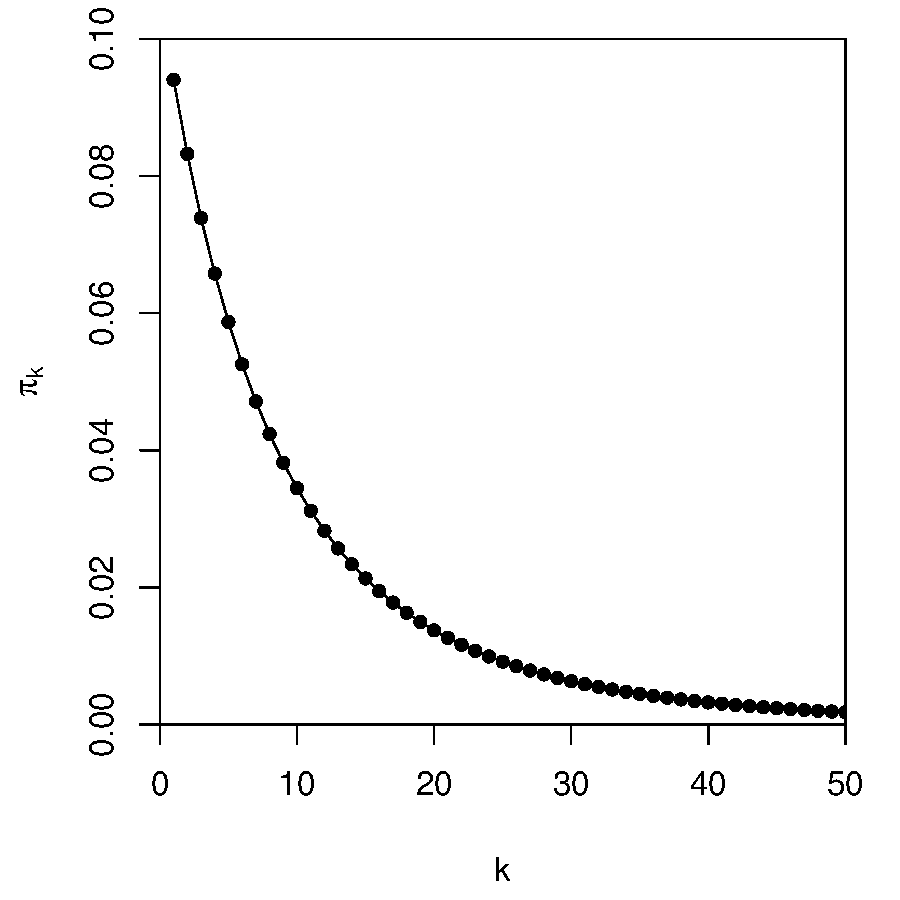
\includegraphics[width=40mm]{img/05-models-zm-2}
    \end{tabular}
  \end{center}
\end{frame}

\begin{frame}
  \frametitle{Zipf-Mandelbrot law as a population model}

  \begin{itemize}
  \item Zipf-Mandelbrot law for type probabilities:
    \[ \pi_i := \frac{C}{(i + b) ^ a} \]
  \item<2-> Two free parameters: $a > 1$ and $b \geq 0$
    \begin{itemize}
    \item[\hand] $C$ is not a parameter but a normalization constant,\\
      needed to ensure that $\sum_i \pi_i = 1$
    \end{itemize}
  \item<3-> Third parameter: $S > 0$ or $S = \infty$
  \item[]
  \item<4-> This is the \h{Zipf-Mandelbrot} population model \citep{Evert:04}
    \begin{itemize}
    \item \hh{ZM} for Zipf-Mandelbrot model ($S = \infty$)
    \item \hh{fZM} for finite Zipf-Mandelbrot model
    \end{itemize}
  \end{itemize}
\end{frame}

\begin{frame}
  \frametitle{The parameters of the Zipf-Mandelbrot model}

  \ungap[1.5]
  \begin{center}
    \begin{tabular}{cc}
      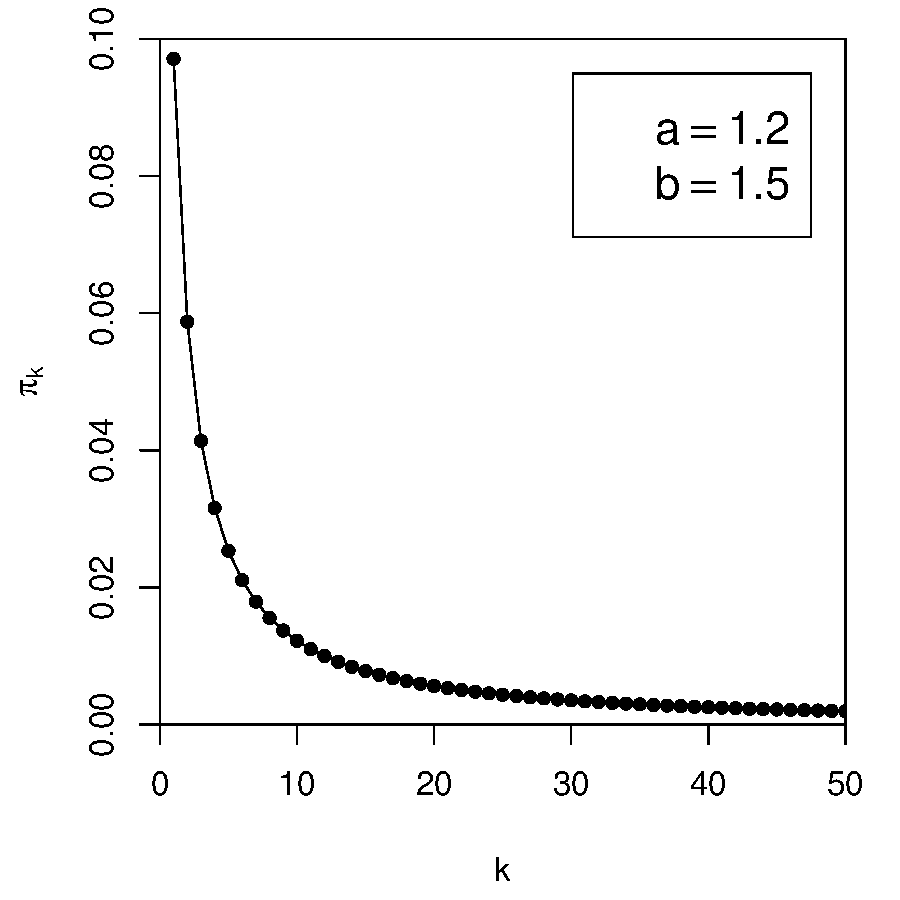
\includegraphics[width=40mm]{img/05-models-zm-param-4} &
      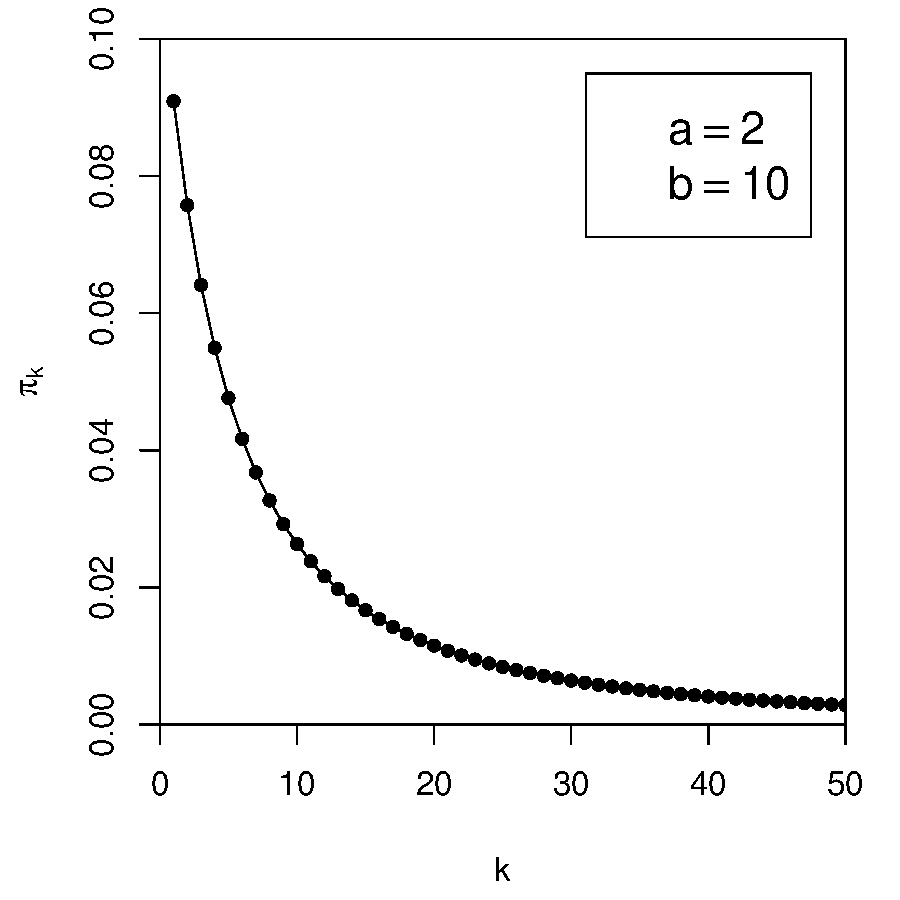
\includegraphics[width=40mm]{img/05-models-zm-param-1} \\
      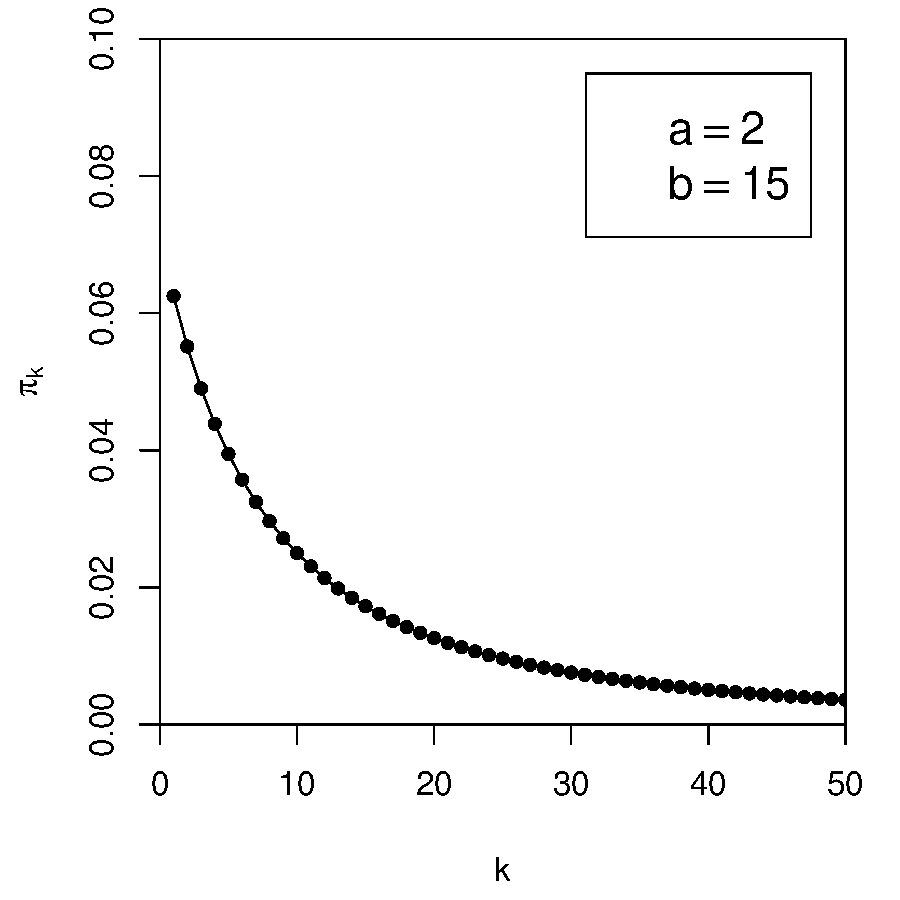
\includegraphics[width=40mm]{img/05-models-zm-param-3} &
      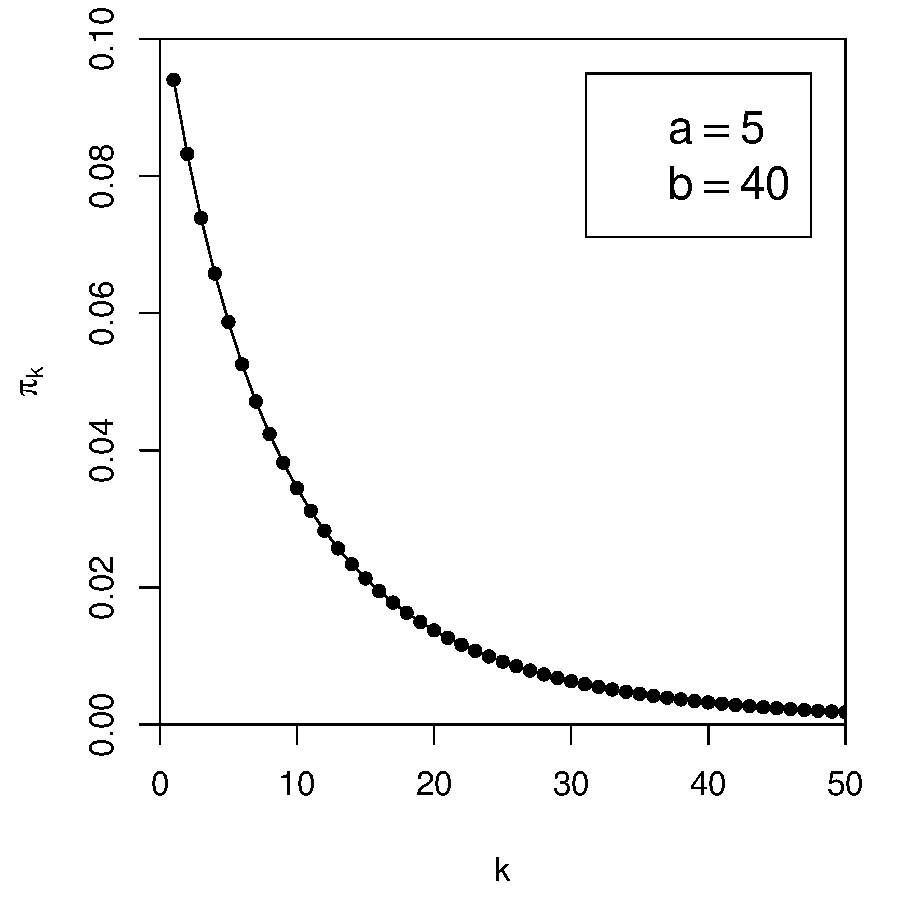
\includegraphics[width=40mm]{img/05-models-zm-param-2}
    \end{tabular}
  \end{center}
\end{frame}

\begin{frame}
  \frametitle{The parameters of the Zipf-Mandelbrot model}

  \ungap[1.5]
  \begin{center}
    \begin{tabular}{cc}
      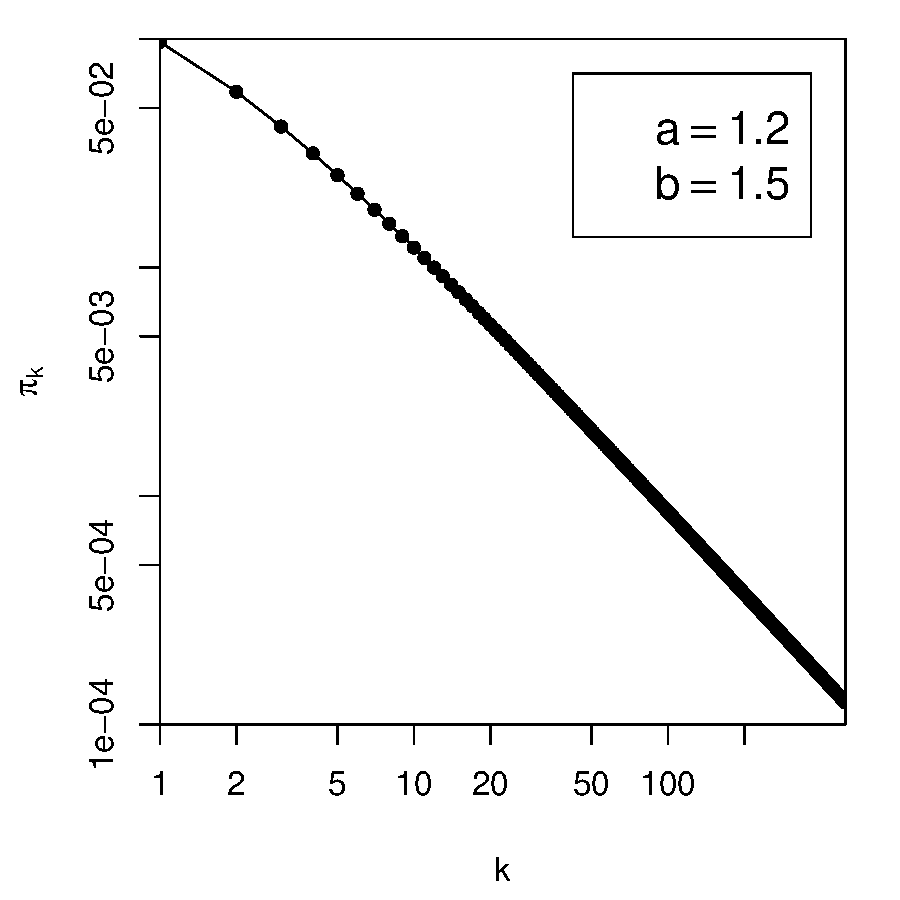
\includegraphics[width=40mm]{img/05-models-zm-log-4} &
      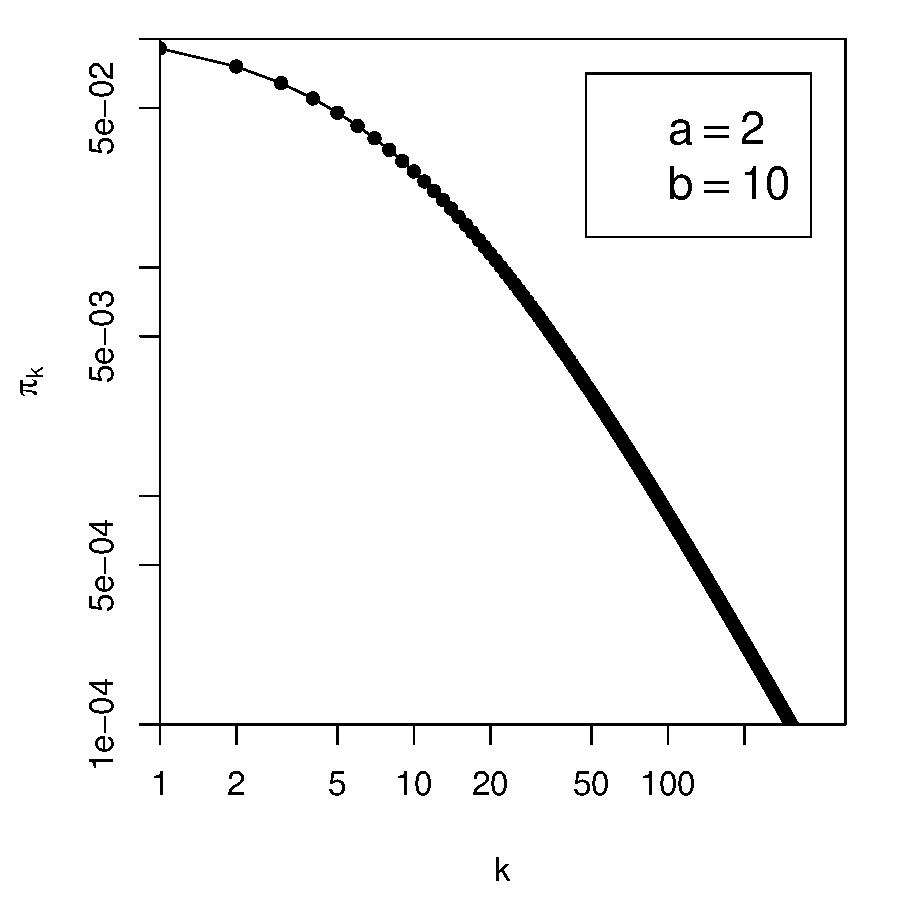
\includegraphics[width=40mm]{img/05-models-zm-log-1} \\
      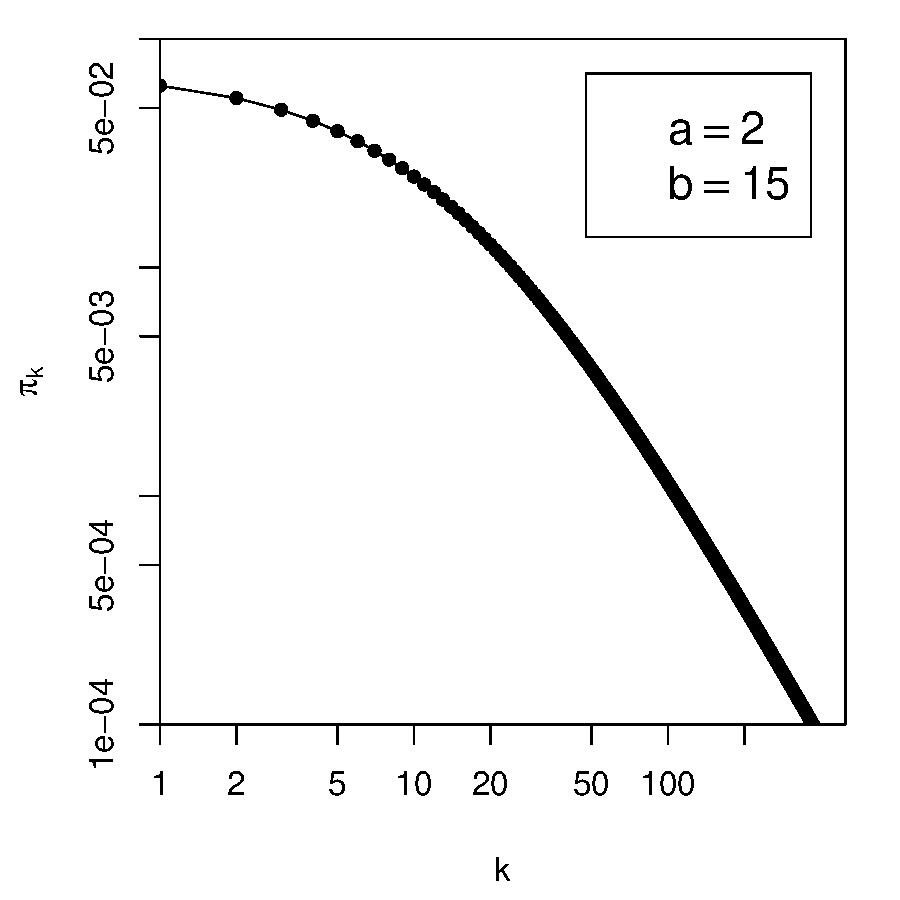
\includegraphics[width=40mm]{img/05-models-zm-log-3} &
      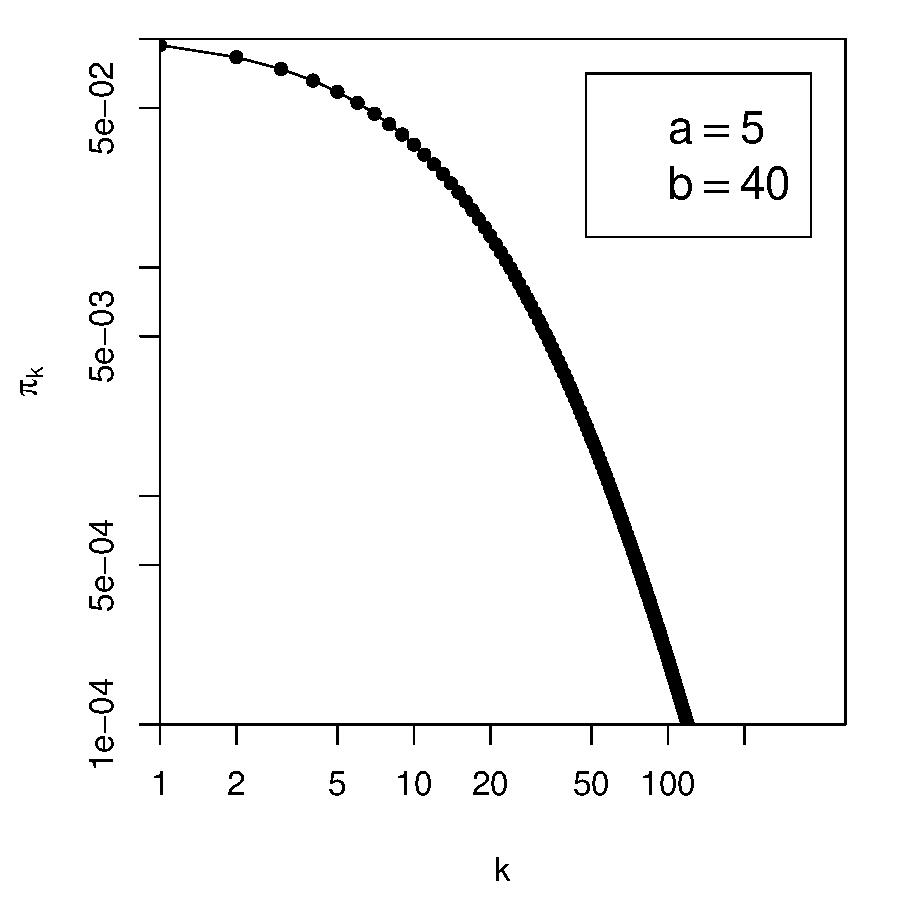
\includegraphics[width=40mm]{img/05-models-zm-log-2}
    \end{tabular}
  \end{center}
\end{frame}

\begin{frame}
  \frametitle{Sampling from a population model}

  Assume we believe that the population we are interested in can be described
  by a Zipf-Mandelbrot model: 
  \begin{center}
    \begin{tabular}{cc}
      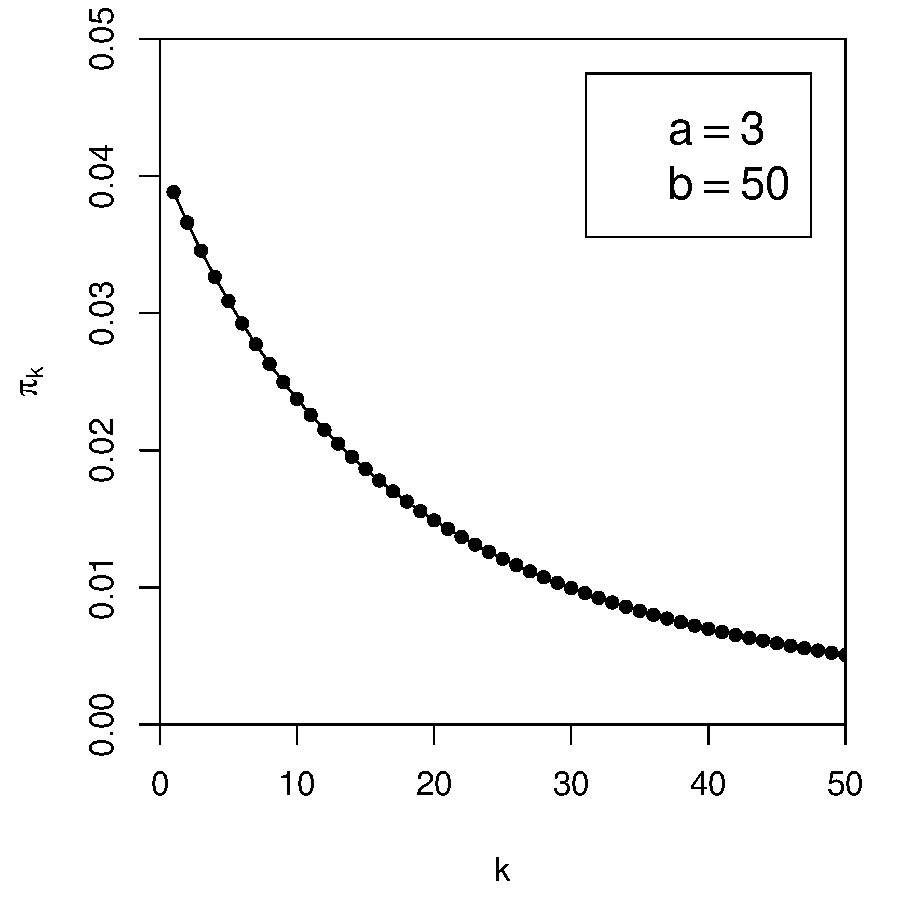
\includegraphics[width=30mm]{img/05-samples-zm-model} &
      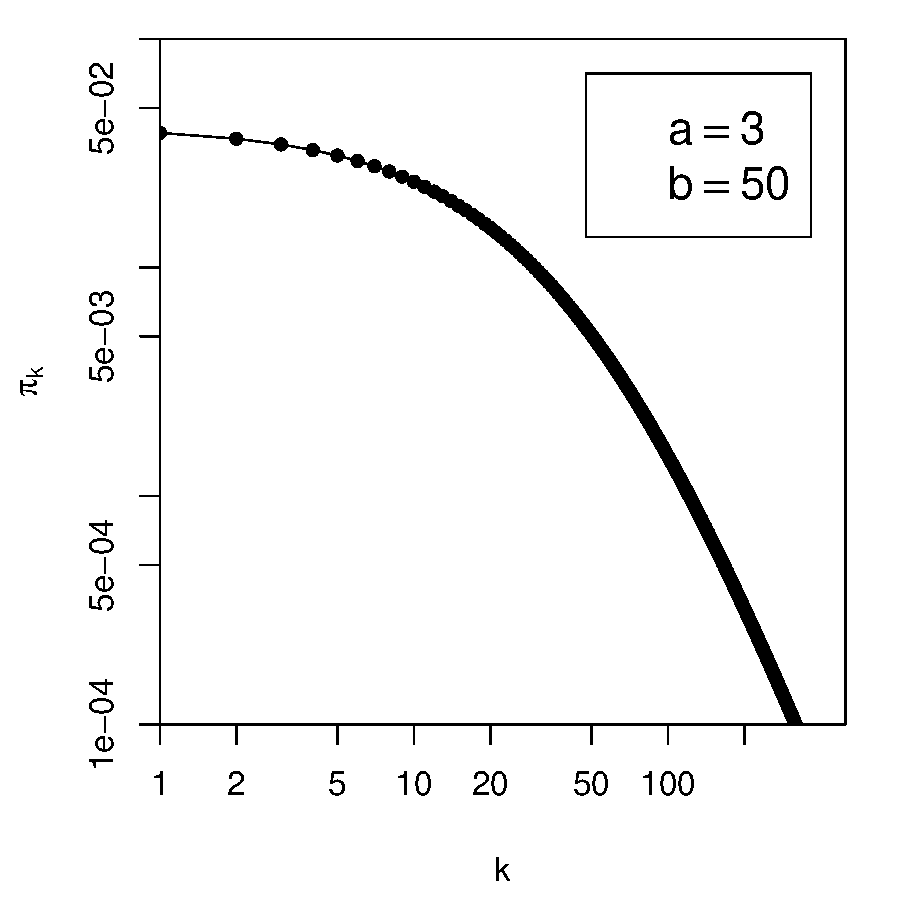
\includegraphics[width=30mm]{img/05-samples-zm-model-log} 
    \end{tabular}
  \end{center}
  
  Use computer simulation to generate random samples:
  \begin{itemize}
  \item Draw $N$ tokens from the population such that in\\
    each step, type $w_i$ has probability $\pi_i$ to be picked
  \item This allows us to make predictions for samples (= corpora)\\
    of arbitrary size $N$
  \end{itemize}
\end{frame}


\begin{frame}
  \frametitle{Sampling from a population model}

  \begin{center}
    \footnotesize
    \begin{tabular}{r *{9}{ @{\hspace{1mm}}r } r}
      \hh{\#1:} &   1 &  42 &  34 &  23 & 108 &  18 &  48 &  18 &   1 & \ldots \\ 
       \pause
      & time & order & room & school & town & course & area & course & time & \ldots \\
       \pause\\
      \hh{\#2:} & 286 &  28 &  23 &  36 &   3 &   4 &   7 &   4 &   8 & \ldots \\ 
       \pause\\
      \hh{\#3:} &   2 &  11 & 105 &  21 &  11 &  17 &  17 &   1 &  16 & \ldots \\ 
       \pause\\
      \hh{\#4:} &  44 &   3 & 110 &  34 & 223 &   2 &  25 &  20 &  28 & \ldots \\ 
       \\
      \hh{\#5:} &  24 &  81 &  54 &  11 &   8 &  61 &   1 &  31 &  35 & \ldots \\ 
      \\
      \hh{\#6:} &   3 &  65 &   9 & 165 &   5 &  42 &  16 &  20 &   7 & \ldots \\ 
      \\
      \hh{\#7:} &  10 &  21 &  11 &  60 & 164 &  54 &  18 &  16 & 203 & \ldots \\ 
      \\
      \hh{\#8:} &  11 &   7 & 147 &   5 &  24 &  19 &  15 &  85 &  37 & \ldots \\
      \\
      \vdots & \vdots & \vdots & \vdots & \vdots & \vdots & \vdots & \vdots & \vdots & \vdots
    \end{tabular}
  \end{center}
\end{frame}

\begin{frame}
  \frametitle{Samples: type frequency list \& spectrum}

  \ungap[1]
  \begin{center}
    \begin{tabular}[t]{r | rr}
      rank $r$ & $f_r$ & type $i$ \\
      \hline
       1 & 37 &  6 \\
       2 & 36 &  1 \\
       3 & 33 &  3 \\
       4 & 31 &  7 \\
       5 & 31 & 10 \\
       6 & 30 &  5 \\
       7 & 28 & 12 \\
       8 & 27 &  2 \\
       9 & 24 &  4 \\
      10 & 24 & 16 \\
      11 & 23 &  8 \\
      12 & 22 & 14 \\
      \vdots & \vdots & \vdots
    \end{tabular}
    \hspace{2cm}
    \begin{tabular}[t]{r | r}
      $m$ & $V_m$ \\
      \hline
       1 & 83 \\
       2 & 22 \\
       3 & 20 \\
       4 & 12 \\
       5 & 10 \\
       6 &  5 \\
       7 &  5 \\
       8 &  3 \\
       9 &  3 \\
      10 &  3 \\
      \vdots & \vdots \\
      \multicolumn{2}{c}{} \\
      \multicolumn{2}{c}{\hh{sample \#1}}
    \end{tabular}
  \end{center}
\end{frame}

\begin{frame}
  \frametitle{Samples: type frequency list \& spectrum}

  \ungap[1]
  \begin{center}
    \begin{tabular}[t]{r | rr}
      rank $r$ & $f_r$ & type $i$ \\
      \hline
       1 & 39 &  2 \\
       2 & 34 &  3 \\
       3 & 30 &  5 \\
       4 & 29 & 10 \\
       5 & 28 &  8 \\
       6 & 26 &  1 \\
       7 & 25 & 13 \\
       8 & 24 &  7 \\
       9 & 23 &  6 \\
      10 & 23 & 11 \\
      11 & 20 &  4 \\
      12 & 19 & 17 \\
      \vdots & \vdots & \vdots
    \end{tabular}
    \hspace{2cm}
    \begin{tabular}[t]{r | r}
      $m$ & $V_m$ \\
      \hline
       1 & 76 \\
       2 & 27 \\
       3 & 17 \\
       4 & 10 \\
       5 &  6 \\
       6 &  5 \\
       7 &  7 \\
       8 &  3 \\
      10 &  4 \\
      11 &  2 \\
      \vdots & \vdots \\
      \multicolumn{2}{c}{} \\
      \multicolumn{2}{c}{\hh{sample \#2}}
    \end{tabular}
  \end{center}
\end{frame}

\begin{frame}
  \frametitle{Random variation in type-frequency lists}

  \ungap[1]
  \begin{tabular}{ccc}
    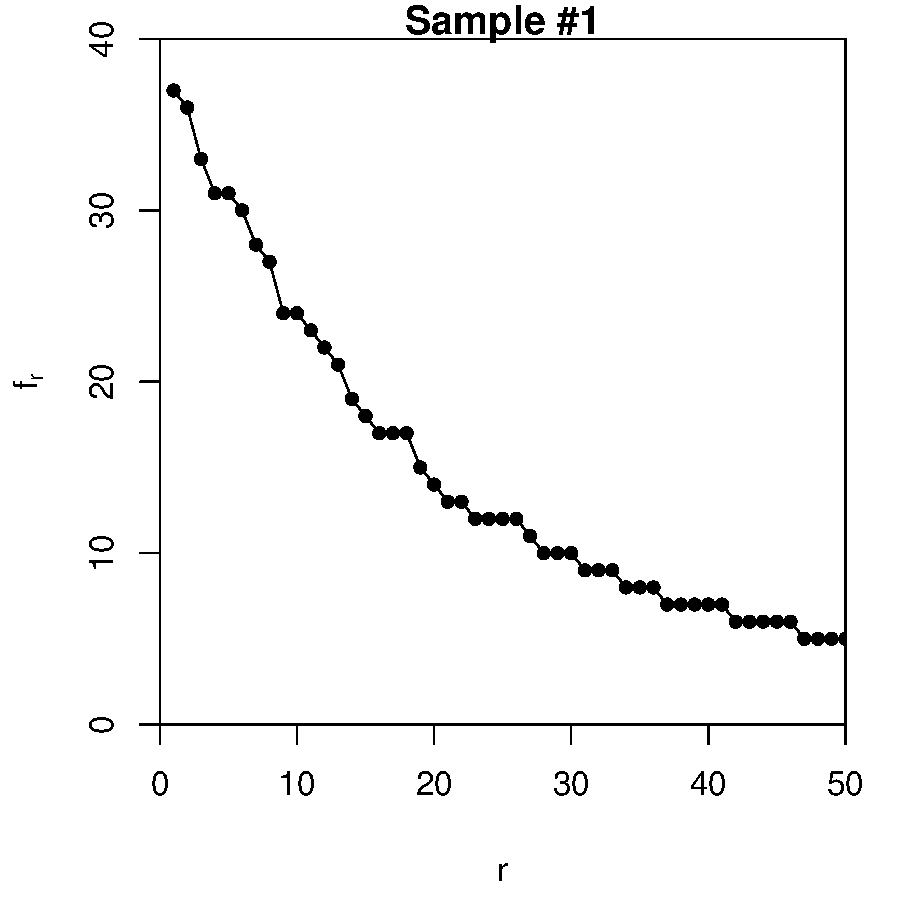
\includegraphics[width=40mm]{img/05-samples-tfl-r-1} &
    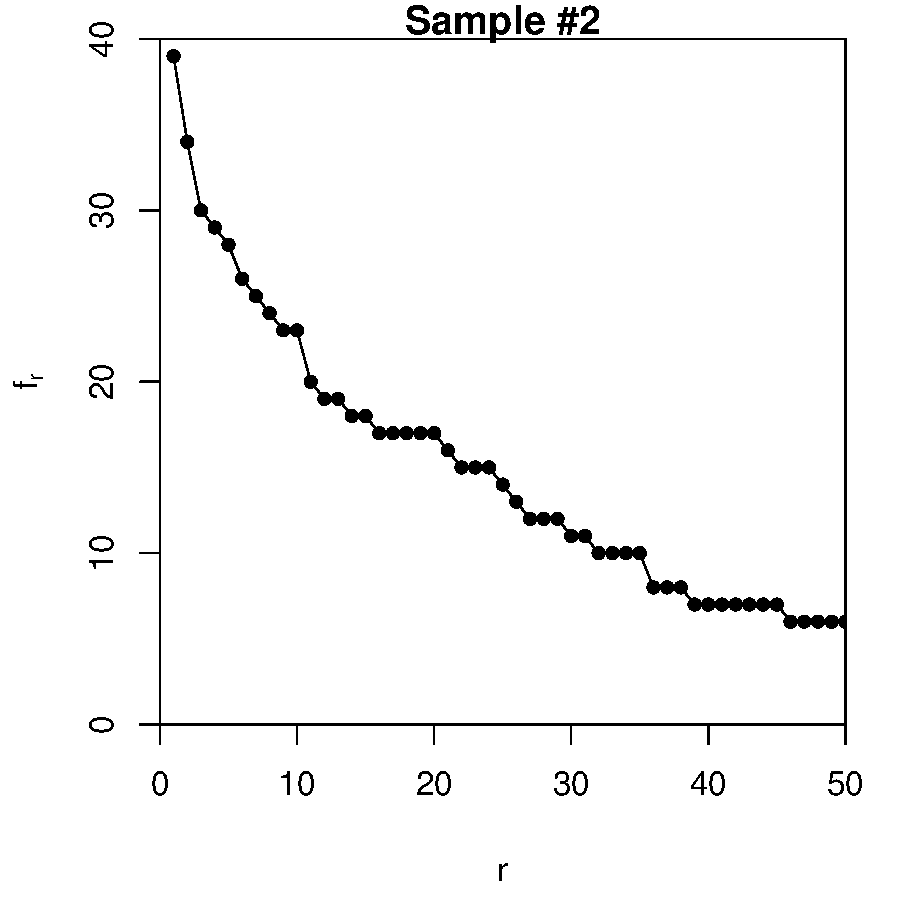
\includegraphics[width=40mm]{img/05-samples-tfl-r-2} &
    \raisebox{2cm}{$r\leftrightarrow f_r$} \\
    
    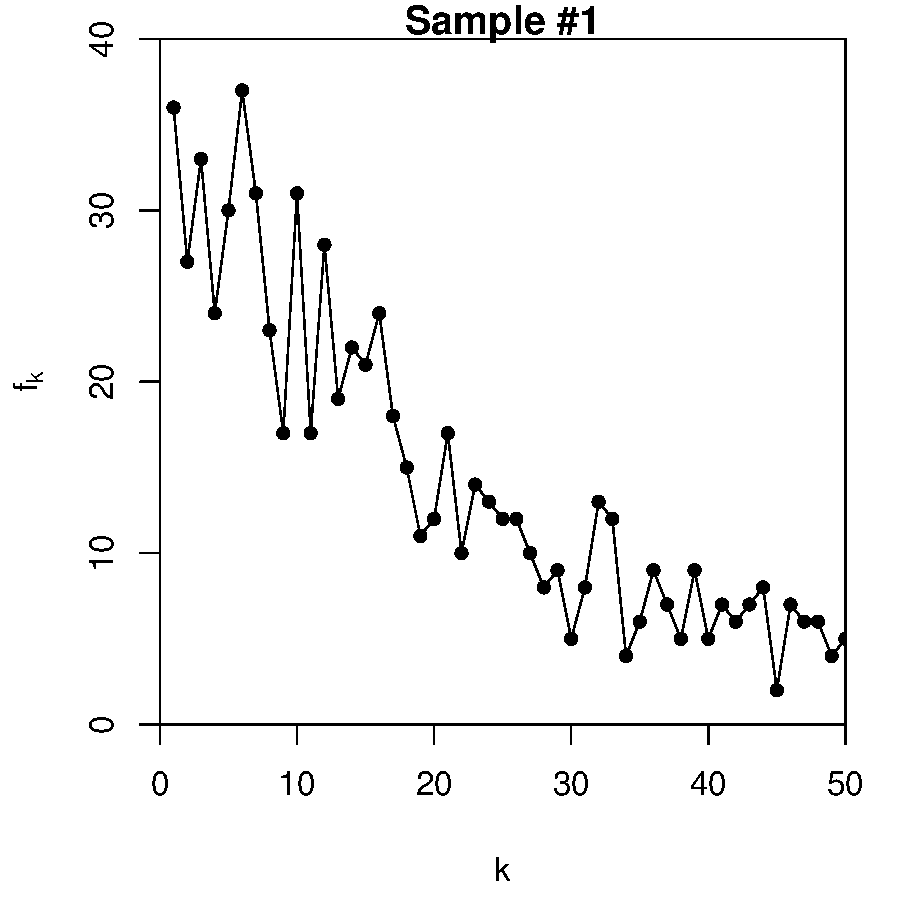
\includegraphics[width=40mm]{img/05-samples-tfl-k-1} &
    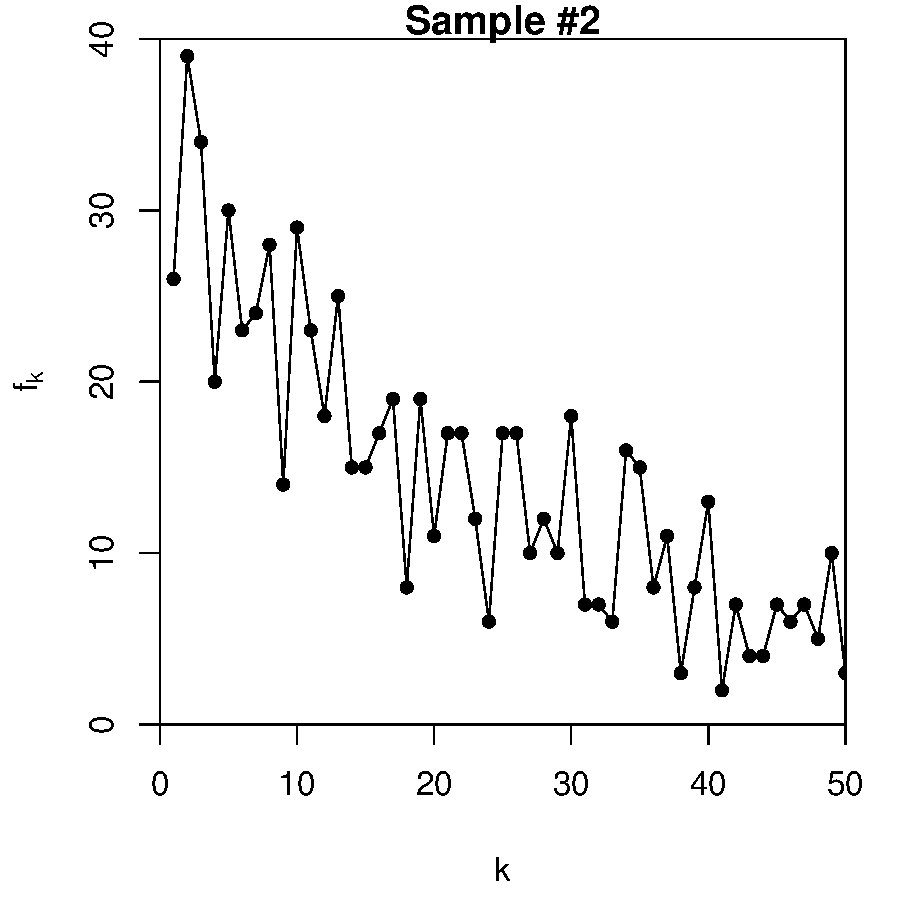
\includegraphics[width=40mm]{img/05-samples-tfl-k-2} &
    \raisebox{2cm}{$i\leftrightarrow f_i$} 
  \end{tabular}
\end{frame}

\begin{frame}
  \frametitle{Random variation: frequency spectrum}

  \ungap[1]
  \begin{center}
    \only<beamer:0| handout:1>{%
      \begin{tabular}{cc}
        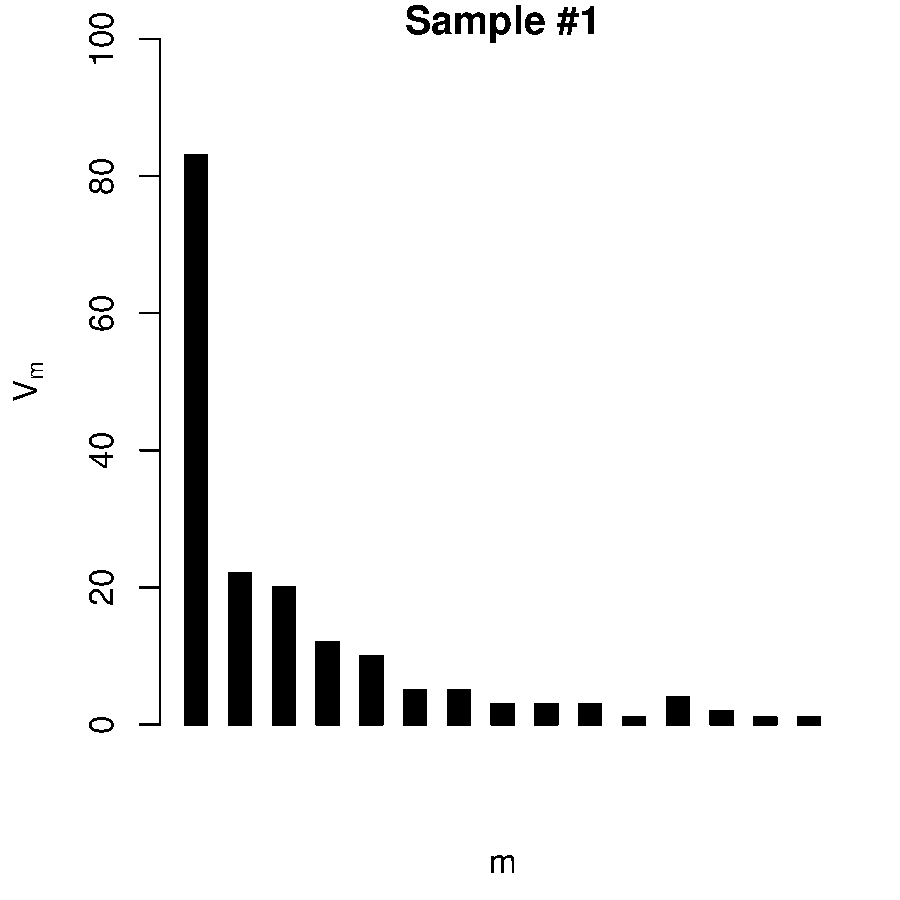
\includegraphics[width=40mm]{img/05-samples-spc-1} &
        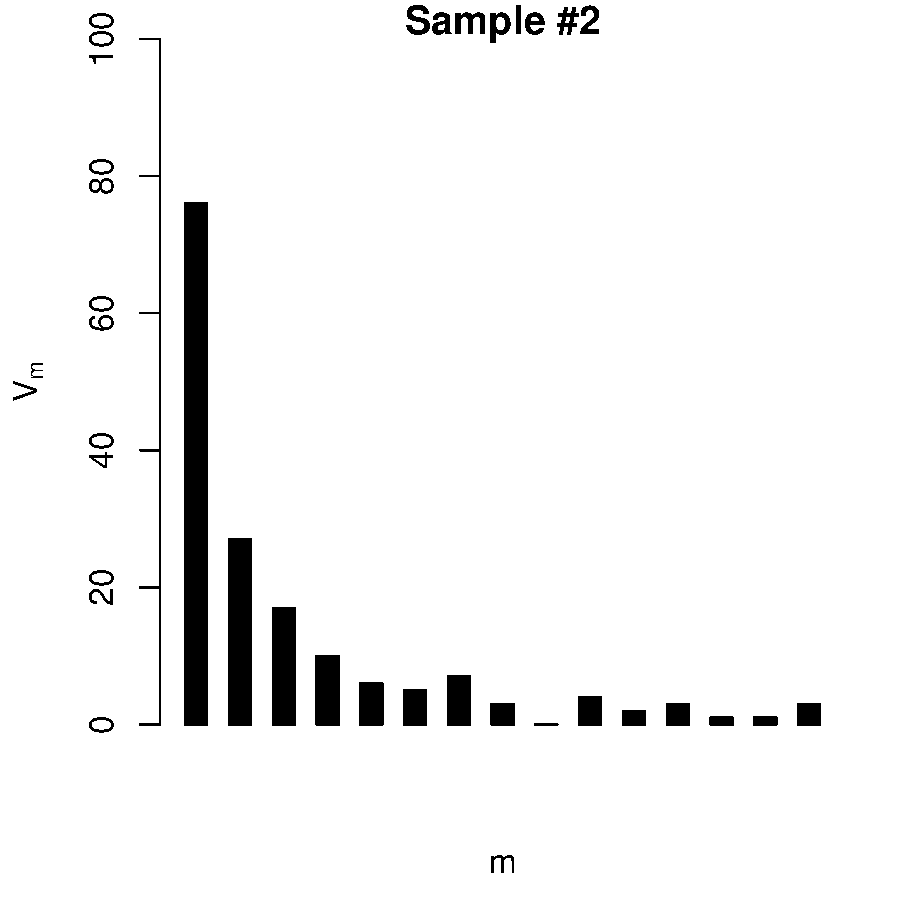
\includegraphics[width=40mm]{img/05-samples-spc-2} \\
        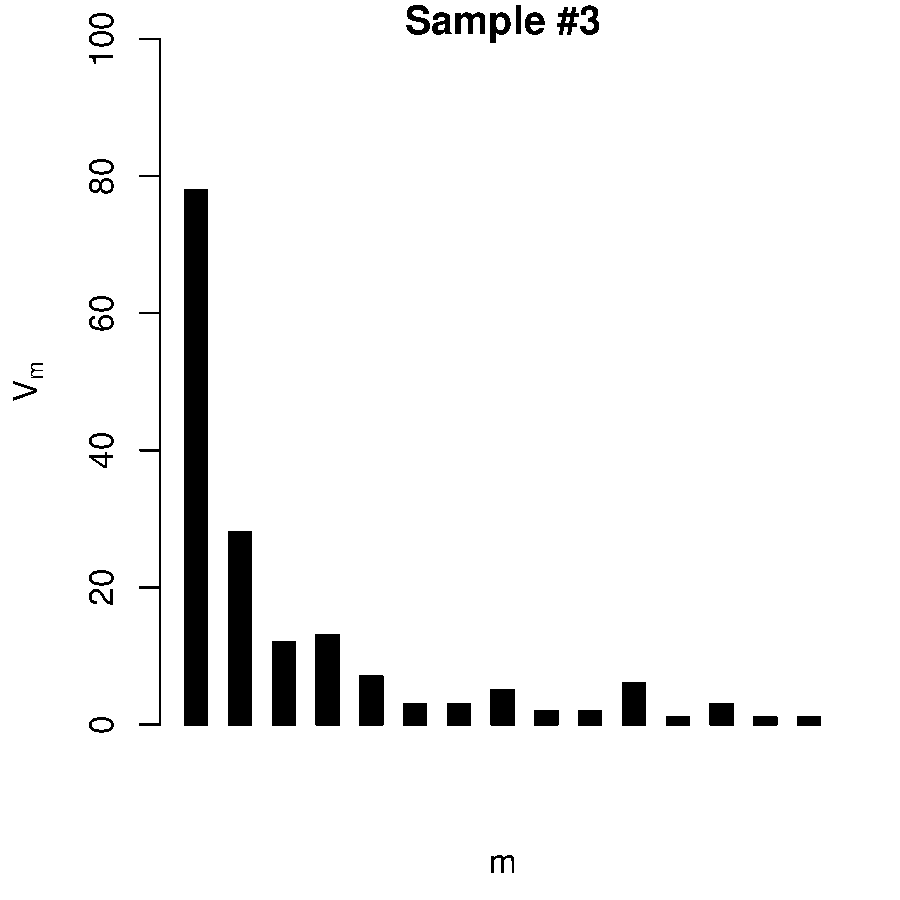
\includegraphics[width=40mm]{img/05-samples-spc-3} &
        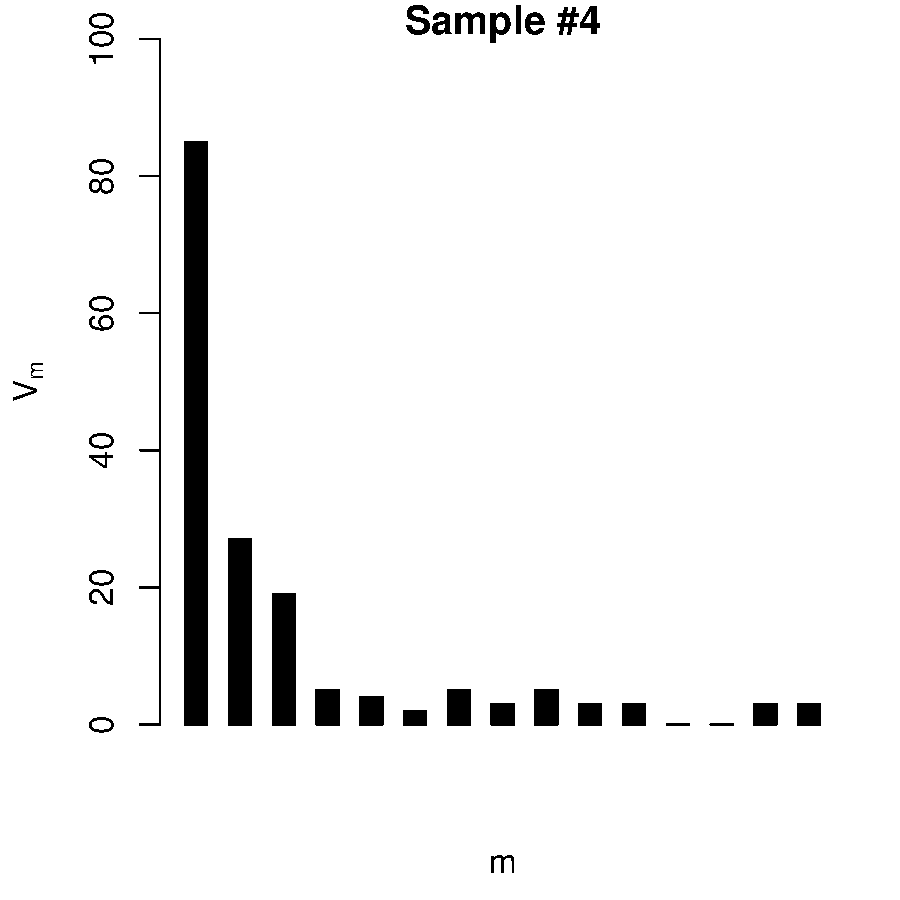
\includegraphics[width=40mm]{img/05-samples-spc-4} 
      \end{tabular}%
    }%
    \only<beamer:1| handout:0>{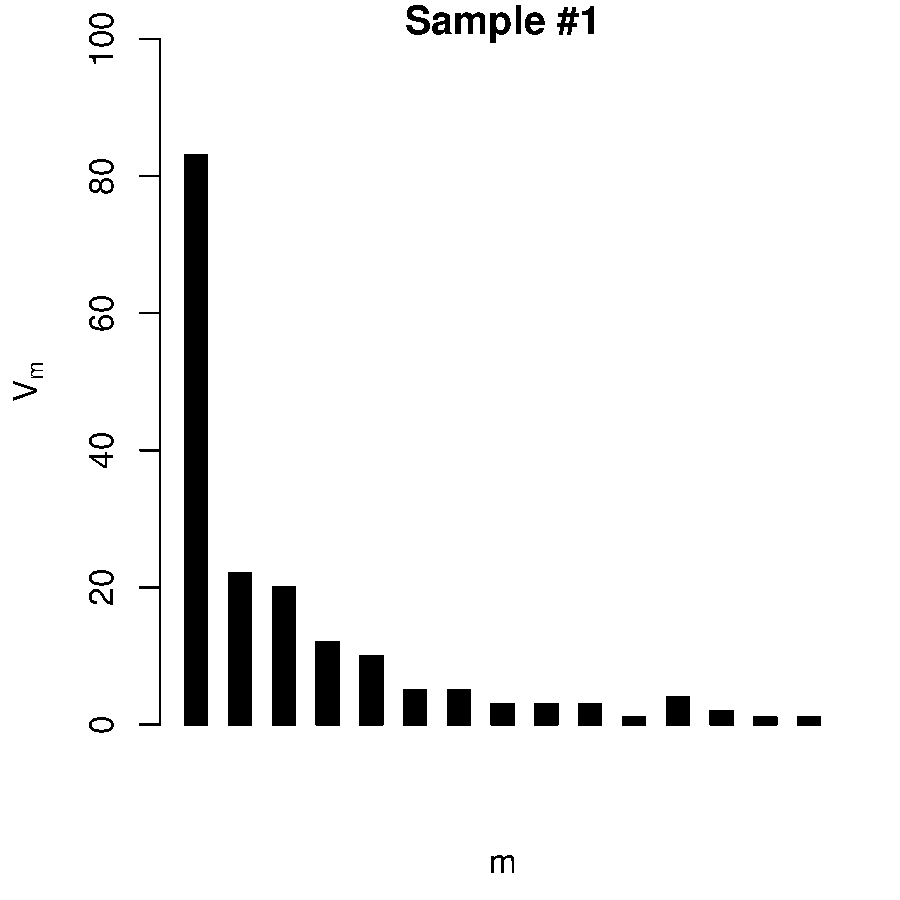
\includegraphics[width=70mm]{img/05-samples-spc-1}}%
    \only<beamer:2| handout:0>{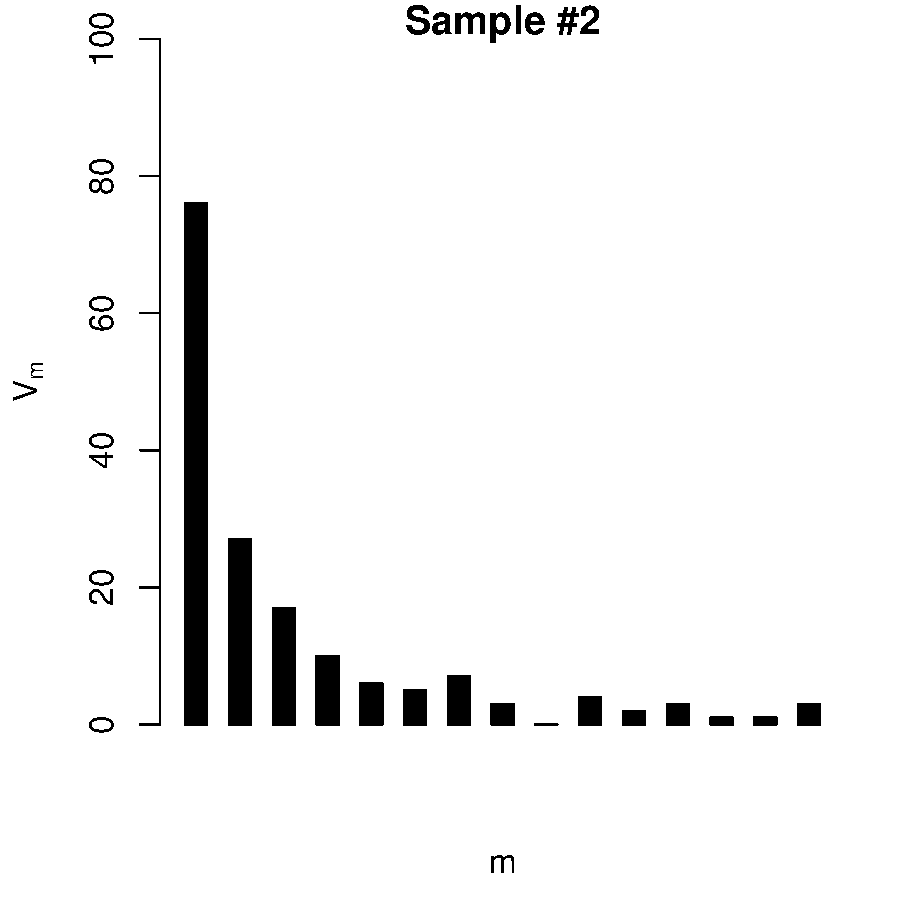
\includegraphics[width=70mm]{img/05-samples-spc-2}}%
    \only<beamer:3| handout:0>{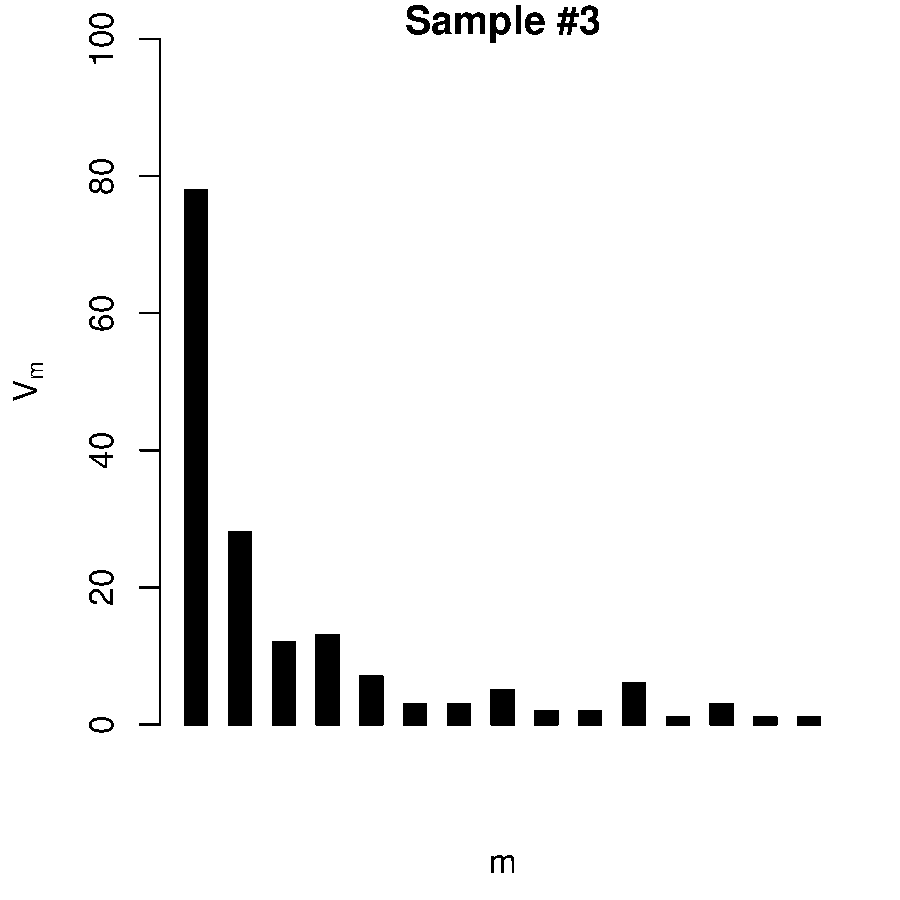
\includegraphics[width=70mm]{img/05-samples-spc-3}}%
    \only<beamer:4| handout:0>{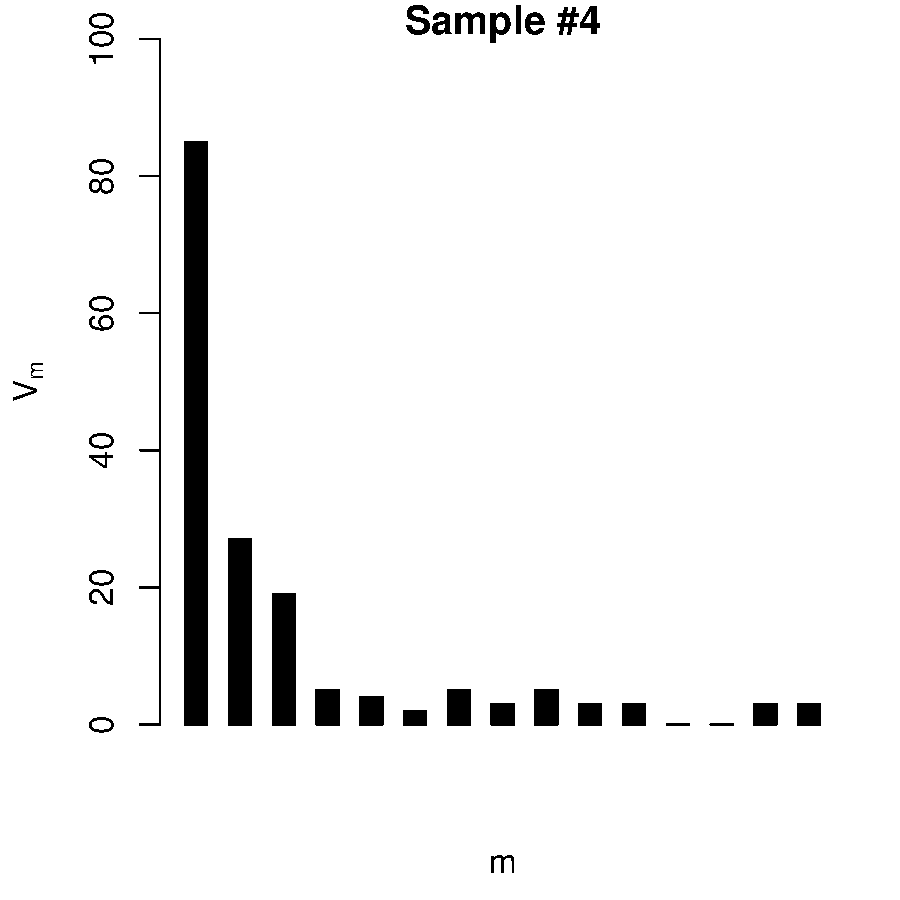
\includegraphics[width=70mm]{img/05-samples-spc-4}}%
  \end{center}
\end{frame}

\begin{frame}
  \frametitle{Random variation: vocabulary growth curve}

  \ungap[1]
  \begin{center}
    \only<beamer:0| handout:1>{%
      \begin{tabular}{cc}
        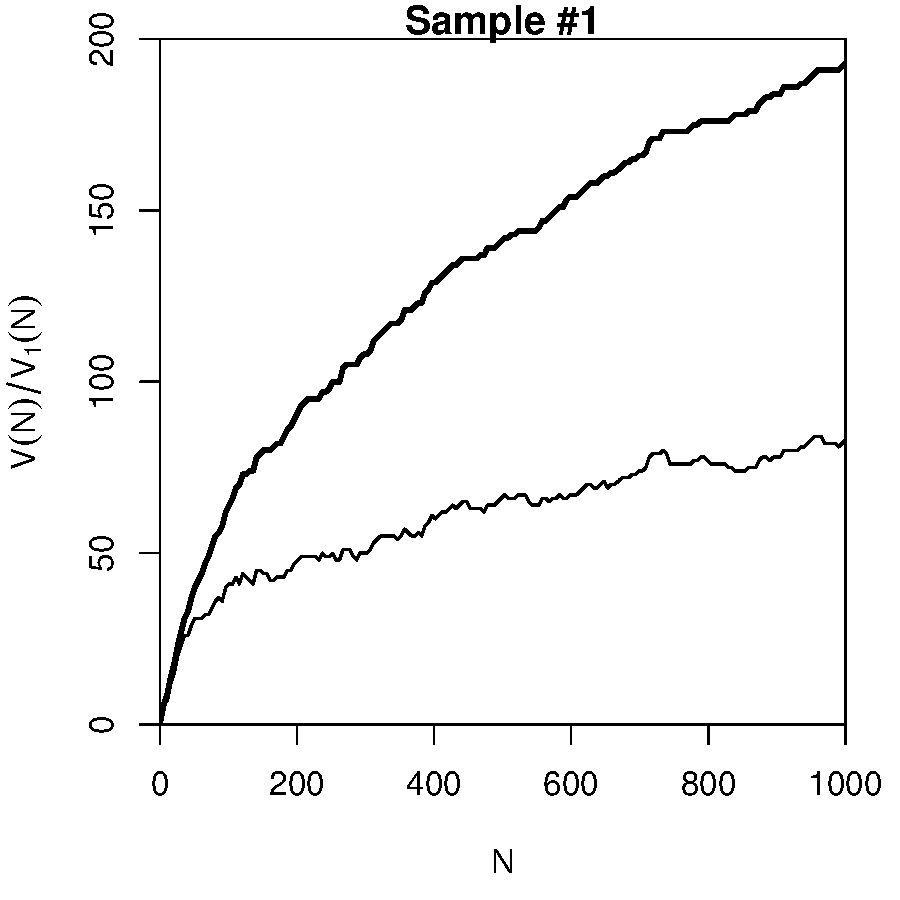
\includegraphics[width=40mm]{img/05-samples-vgc-1} &
        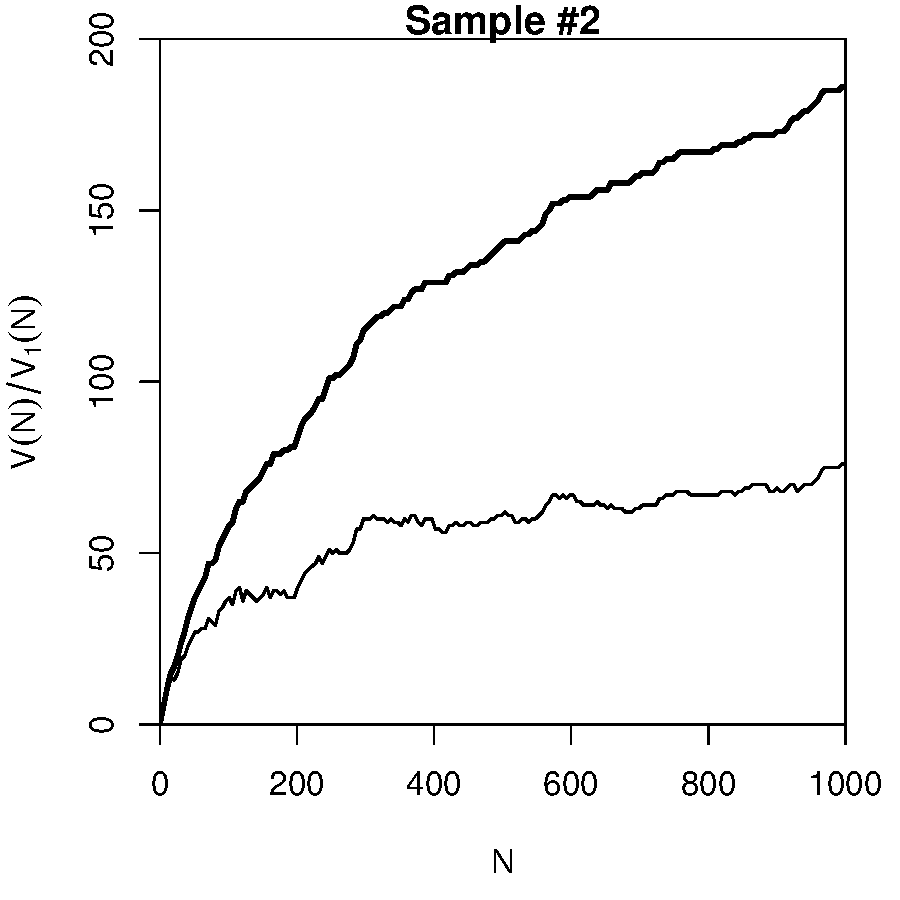
\includegraphics[width=40mm]{img/05-samples-vgc-2} \\
        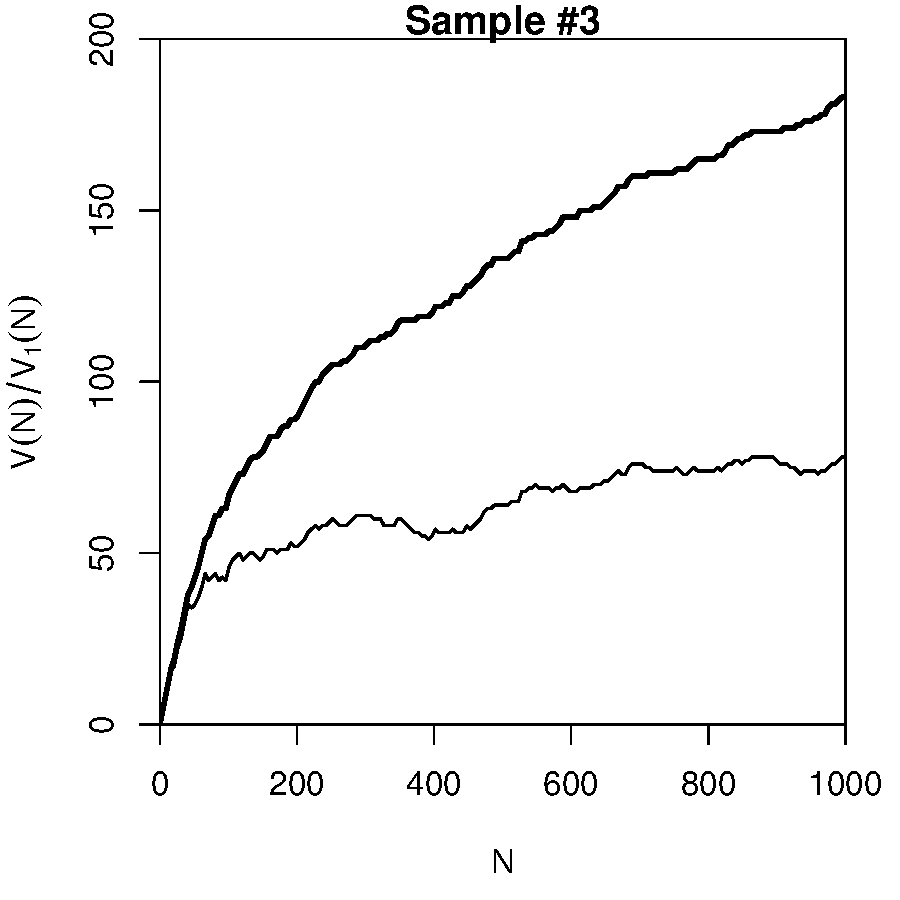
\includegraphics[width=40mm]{img/05-samples-vgc-3} &
        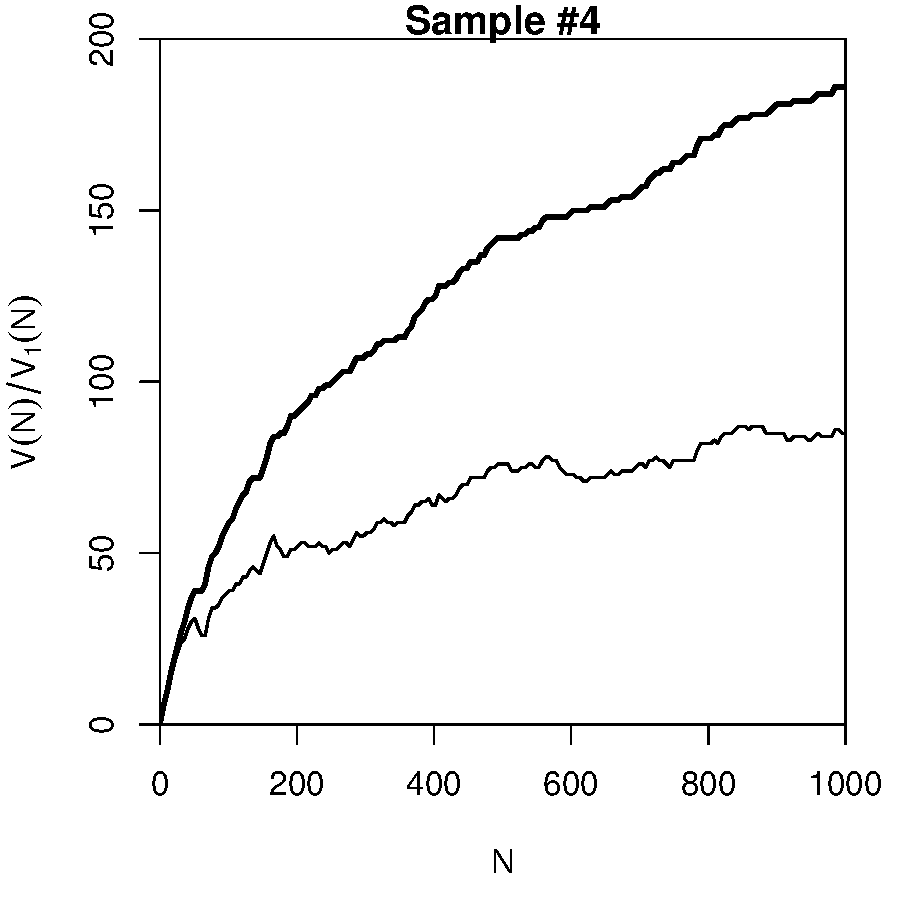
\includegraphics[width=40mm]{img/05-samples-vgc-4} 
      \end{tabular}%
    }%
    \only<beamer:1| handout:0>{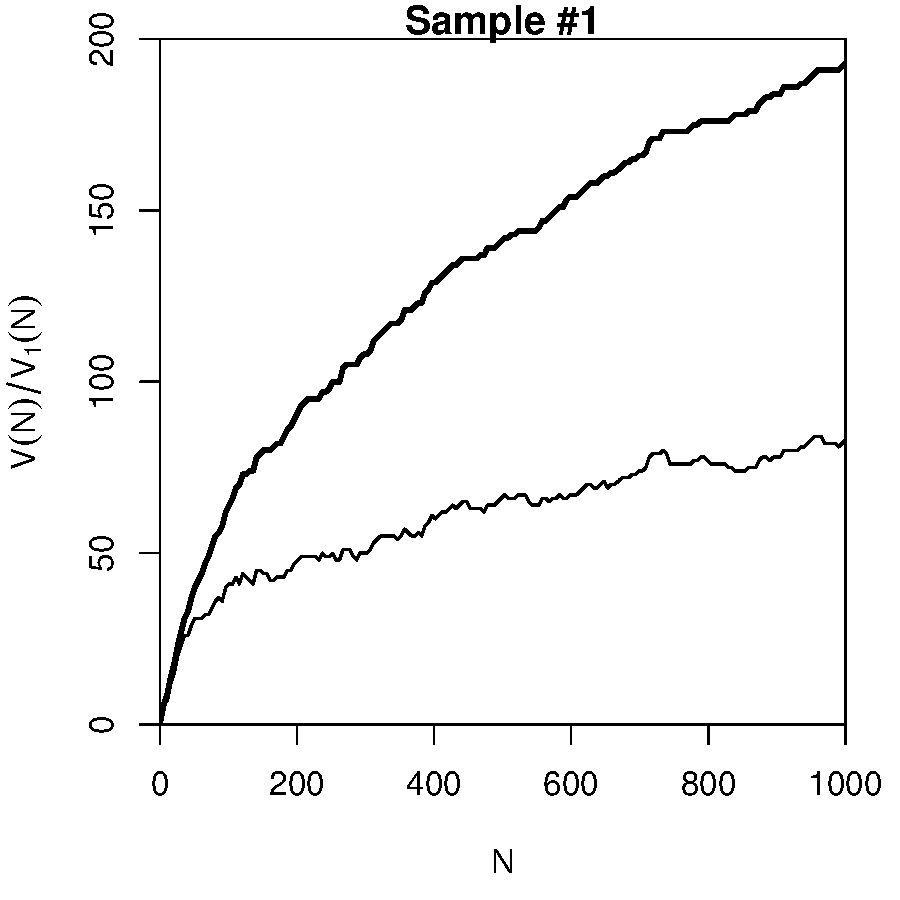
\includegraphics[width=70mm]{img/05-samples-vgc-1}}%
    \only<beamer:2| handout:0>{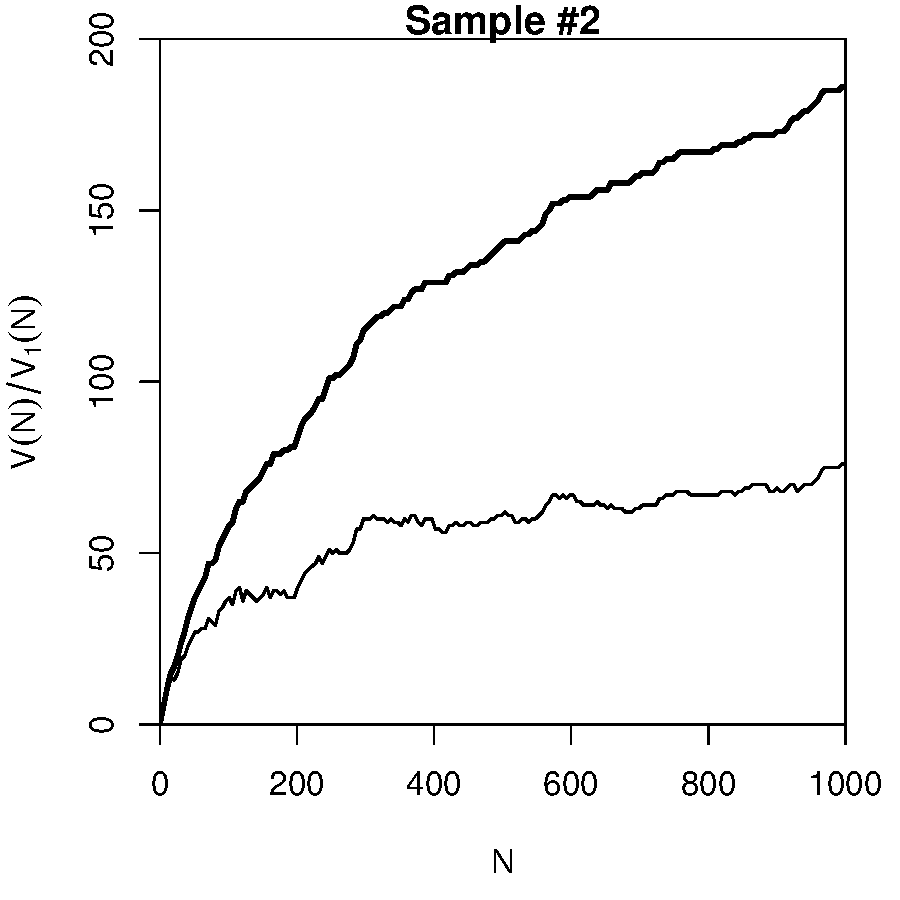
\includegraphics[width=70mm]{img/05-samples-vgc-2}}%
    \only<beamer:3| handout:0>{\includegraphics[width=70mm]{img/05-samples-vgc-3}}%
    \only<beamer:4| handout:0>{\includegraphics[width=70mm]{img/05-samples-vgc-4}}%
  \end{center}
\end{frame}


\begin{frame}
  \frametitle{Expected values}

  \begin{itemize}
  \item There is no reason why we should choose a particular sample to compare
    to the real data or make a prediction -- each one is equally likely or
    unlikely
  \item Take the average over a large number of samples, called \h{expected
      value} or \h{expectation} in statistics
  \item[]
  \item Notation: $\text{E}\bigl[V(N)\bigr]$ and $\text{E}\bigl[V_m(N)\bigr]$
    \begin{itemize}
    \item indicates that we are referring to expected values for a sample of
      size $N$
    \item rather than to the specific values $V$ and $V_m$\\
      observed in a particular sample or a real-world data set
    \item[]
    \end{itemize}
  \item Expected values can be calculated efficiently \emph{without}
    generating thousands of random samples
  \end{itemize}
\end{frame}

\begin{frame}
  \frametitle{The expected frequency spectrum}

  \ungap[1]
  \begin{center}
    \only<beamer:0| handout:1>{%
      \begin{tabular}{cc}
        \includegraphics[width=40mm]{img/05-samples-spc-exp-vs-sample-1} &
        \includegraphics[width=40mm]{img/05-samples-spc-exp-vs-sample-2} \\
        \includegraphics[width=40mm]{img/05-samples-spc-exp-vs-sample-3} &
        \includegraphics[width=40mm]{img/05-samples-spc-exp-vs-sample-4} 
      \end{tabular}%
    }%
    \only<beamer:1| handout:0>{\includegraphics[width=70mm]{img/05-samples-spc-exp-vs-sample-1}}%
    \only<beamer:2| handout:0>{\includegraphics[width=70mm]{img/05-samples-spc-exp-vs-sample-2}}%
    \only<beamer:3| handout:0>{\includegraphics[width=70mm]{img/05-samples-spc-exp-vs-sample-3}}%
    \only<beamer:4| handout:0>{\includegraphics[width=70mm]{img/05-samples-spc-exp-vs-sample-4}}%
  \end{center}
\end{frame}

\begin{frame}
  \frametitle{The expected vocabulary growth curve}

  \ungap[1]
  \begin{center}
    \begin{tabular}{c @{} c}
      \includegraphics[width=50mm]{img/05-samples-vgc-exp-vs-samples} &
      \includegraphics[width=50mm]{img/05-samples-vgc-V1-exp-vs-samples}
    \end{tabular}
  \end{center}
\end{frame}

\begin{frame}
  \frametitle{Prediction intervals for the expected VGC}

  \ungap[1]
  \begin{center}
    \begin{tabular}{c @{} c}
      \includegraphics[width=50mm]{img/05-samples-vgc-exp-vs-samples-conf} &
      \includegraphics[width=50mm]{img/05-samples-vgc-V1-exp-vs-samples-conf}
    \end{tabular}
  \end{center}

  ``Confidence intervals'' indicate predicted sampling distribution:%
  \begin{itemize}
  \item[\hand] for 95\% of samples generated by the LNRE model, VGC will fall within the range delimited by the thin red lines
  \end{itemize}

\end{frame}

\begin{frame}<beamer:1-7| handout:1-3,7>
  \frametitle{Parameter estimation by trial \& error}

  \begin{center}
    \begin{tabular}{c @{} c}
      \only<beamer:1| handout:1>{\includegraphics[width=50mm]{img/05-estimation-spc-1}}%
      \only<beamer:2| handout:2>{\includegraphics[width=50mm]{img/05-estimation-spc-2}}%
      \only<beamer:3| handout:3>{\includegraphics[width=50mm]{img/05-estimation-spc-3}}%
      \only<beamer:4| handout:0>{\includegraphics[width=50mm]{img/05-estimation-spc-1}}%
      \only<beamer:5| handout:0>{\includegraphics[width=50mm]{img/05-estimation-spc-4}}%
      \only<beamer:6| handout:0>{\includegraphics[width=50mm]{img/05-estimation-spc-5}}%
      \only<beamer:7| handout:7>{\includegraphics[width=50mm]{img/05-estimation-spc-6}}%
      &
      \only<beamer:1| handout:1>{\includegraphics[width=50mm]{img/05-estimation-vgc-1}}%
      \only<beamer:2| handout:2>{\includegraphics[width=50mm]{img/05-estimation-vgc-2}}%
      \only<beamer:3| handout:3>{\includegraphics[width=50mm]{img/05-estimation-vgc-3}}%
      \only<beamer:4| handout:0>{\includegraphics[width=50mm]{img/05-estimation-vgc-1}}%
      \only<beamer:5| handout:0>{\includegraphics[width=50mm]{img/05-estimation-vgc-4}}%
      \only<beamer:6| handout:0>{\includegraphics[width=50mm]{img/05-estimation-vgc-5}}%
      \only<beamer:7| handout:7>{\includegraphics[width=50mm]{img/05-estimation-vgc-6}}%
    \end{tabular}
  \end{center}
\end{frame}

\begin{frame}
  \frametitle{Automatic parameter estimation}
  % \framesubtitle{Minimisation of suitable cost function for frequency spectrum}

  \begin{center}
    \begin{tabular}{c @{} c}
      \includegraphics[width=50mm]{img/05-estimation-spc-estimated} &
      \includegraphics[width=50mm]{img/05-estimation-vgc-estimated} 
    \end{tabular}
  \end{center}

  \ungap[1]
  \begin{itemize}
    \item By trial \& error we found $a=2.0$ and $b=550$
    \item Automatic estimation procedure: $a=2.39$ and $b=1968$
  \end{itemize}
\end{frame}


%%%%%%%%%%%%%%%%%%%%%%%%%%%%%%%%%%%%%%%%%%%%%%%%%%%%%%%%%%%%%%%%%%%%%%%%
\subsection{The mathematics of LNRE}

\begin{frame}
  \frametitle{The sampling model}

  \begin{itemize}
  \item Draw random sample of $N$ tokens from LNRE population
  \item Sufficient statistic: set of type frequencies $\set{f_i}$
    \begin{itemize}
    \item because tokens of random sample have no ordering
    \end{itemize}
  \item Joint \hh{multinomial} distribution of $\set{f_i}$:
    \[
      \pC{\set{f_i = k_i}}{N} =
      \frac{N!}{k_1! \cdots k_S!} \pi_1^{k_1} \cdots \pi_S^{k_S}
    \]
  \item<2-> \h{Approximation:} do not condition on fixed sample size $N$
    \begin{itemize}
    \item $N$ is now the average (expected) sample size
    \end{itemize}
  \item<2-> Random variables $f_i$ have \hh{independent Poisson} distributions:
    \[
      \p{f_i = k_i} = e^{-N\pi_i} \frac{(N\pi_i)^{k_i}}{k_i!}
    \]
  \end{itemize}
\end{frame}

\begin{frame}
  \frametitle{Frequency spectrum}

  \begin{itemize}
  \item Key problem: we cannot determine $f_i$ in observed sample
    \begin{itemize}
    \item because we don't know which type $w_i$ is
    \item recall that population ranking $f_i$ $\neq$ Zipf ranking $f_r$
    \end{itemize}
  \item Use spectrum $\set{V_m}$ and sample size $V$ as statistics
    \begin{itemize}
    \item contains all information we have about observed sample
    \end{itemize}
  \item<2-> Can be expressed in terms of indicator variables
    \begin{align*}
      \IV{f_i = m} &=
      \begin{cases}
        1 & f_i = m\\
        0 & \text{otherwise}
      \end{cases}\\
      \visible<3->{V_m &= \sum_{i=1}^S \IV{f_i = m}} \\
      \visible<4->{V &= \sum_{i=1}^S \IV{f_i > 0} = \sum_{i=1}^S \bigl( 1 - \IV{f_i = 0} \bigr)}
    \end{align*}
  \end{itemize}
\end{frame}

\begin{frame}
  \frametitle{The expected spectrum}

  \begin{itemize}
  \item It is easy to compute expected values for the frequency spectrum (and
    variances because the $f_i$ are independent)
    \begin{align*}
      \Exp{\IV{f_i = m}} &= \p{f_i = m} = e^{-N\pi_i} \frac{(N\pi_i)^m}{m!}\\
      \visible<2->{\Exp{V_m} &= \sum_{i=1}^S \Exp{\IV{f_i = m}} = \sum_{i=1}^S e^{-N\pi_i} \frac{(N\pi_i)^m}{m!}}\\
      \visible<3->{\Exp{V} &= \sum_{i=1}^S \bigExp{1 - \IV{f_i = 0}} = \sum_{i=1}^S \bigl( 1 - e^{-N\pi_i} \bigr)}
    \end{align*}
  \item<4-> NB: $V_m$ and $V$ are \primary{not independent} because they are
    derived from the same random variables $f_i$
  \end{itemize}
\end{frame}

\begin{frame}
  \frametitle{Sampling distribution of $V_m$ and $V$}

  \begin{itemize}
  \item Joint sampling distribution of $\set{V_m}$ and $V$ is complicated
  \item \h{Approximation:} $V$ and $\set{V_m}$ asymptotically follow a \hh{multivariate normal} distribution
    \begin{itemize}
    \item motivated by the multivariate central limit theorem:\\ sum of many independent variables $\IV{f_i = m}$
    \end{itemize}
  \item Usually limited to first spectrum elements, e.g.\ $V_1, \ldots, V_{15}$
    \begin{itemize}
    \item approximation of discrete $V_m$ by continuous distribution
      suitable only if $\Exp{V_m}$ is sufficiently large
    \end{itemize}
  \item<2-> Parameters of multivariate normal:
    $\pmb{\mu} = (\Exp{V}, \Exp{V_1}, \Exp{V_2}, \ldots)$ and $\pmb{\Sigma}$ = covariance matrix
    \[
      \bigp{(V, V_1, \ldots, V_k) = \mathbf{v}} \sim
      \frac{
        e^{-\frac12 (\mathbf{v} - \pmb{\mu})^T \pmb{\Sigma}^{-1} (\mathbf{v} - \pmb{\mu})}
      }{\small
        \sqrt{(2\pi)^{k+1} \det \pmb{\Sigma}}
      }
    \]
  \end{itemize}
\end{frame}

\begin{frame}
  \frametitle{Type density function}

  \begin{itemize}
  \item Discrete sums of probabilities in $\Exp{V}$, $\Exp{V_m}$, $\ldots$ are inconvenient and computationally expensive
  \item \h{Approximation:} continuous \h{type density function} $g(\pi)$
    \begin{align*}
      \abs{\setdef{w_i}{a \leq \pi_i \leq b}}
      &= \int_a^b g(\pi) \dpi\\
      \sum \setdef{\pi_i}{a \leq \pi_i \leq b}
      &= \int_a^b \pi g(\pi) \dpi
    \end{align*}
  \item<2-> Normalization constraint:
    \[
      \int_0^{\infty} \pi g(\pi) \dpi = 1
    \]
  \item<2-> Good approximation for low-probability types, but probability mass of $w_1, w_2, \ldots$ ``smeared out'' over range
  \end{itemize}
\end{frame}

\begin{frame}
  \frametitle{Type density function}

  \centering
  \begin{tikzpicture}
    \useasboundingbox (0, 0) rectangle (11, 7) ;
    \node[anchor=south west] at (0, 0) {\includegraphics[width=11cm]{../plots/lnre_tdf_vs_prob}} ;
    \visible<2->{
      \node[anchor=south west] at (4.5, 3) {\includegraphics[width=7cm]{../plots/lnre_pdf_vs_prob}} ;
    }
  \end{tikzpicture}
\end{frame}

\begin{frame}
  \frametitle{ZM and fZM as LNRE models}

  \begin{itemize}
  \item Discrete Zipf-Mandelbrot population
    \[
      \pi_i := \frac{C}{(i + b) ^ a} \quad \text{for } i = 1, \ldots, S
    \]
  \item<2-> Corresponding type density function \citep{Evert:04}
    \[
      g(\pi) =
      \begin{cases}
        C\cdot \pi^{-\alpha-1} & A \leq \pi \leq B\\
        0 & \text{otherwise}
      \end{cases}
    \]
    \onslide<3->
    with parameters
    \begin{itemize}
    \item $\primary{\alpha} = 1 / a$ ($0 < \alpha < 1$)
    \item $\primary{B} = (1 - \alpha) / (b \cdot \alpha)$
    \item $0 \leq \primary{A} < B$ determines $S$ (ZM with $S = \infty$ for $A = 0$)
    \item[\hand] $C$ is a normalization factor, not a parameter
    \end{itemize}
  \end{itemize}
\end{frame}

\begin{frame}[c]
  \frametitle{ZM and fZM as LNRE models}

  \centering
  \only<beamer:1| handout:0>{\includegraphics[width=11cm]{../plots/lnre_tdf_zm}}%
  \only<beamer:2| handout:1>{\includegraphics[width=11cm]{../plots/lnre_tdf_fzm}}%
\end{frame}

\begin{frame}
  \frametitle{Expectations as integrals}

  \begin{itemize}
  \item Expected values can now be expressed as integrals over $g(\pi)$
    \begin{align*}
      \Exp{V_m} &= \int_0^{\infty} \frac{(N\pi)^m}{m!} e^{-N\pi} g(\pi) \dpi\\
      \Exp{V} &= \int_0^{\infty} \bigl( 1 - e^{-N\pi} \bigr) g(\pi) \dpi
    \end{align*}
  \item<2-> Reduce to simple closed form for ZM with $b = 0$ (\so $B = \infty$)
    \begin{align*}
      \Exp{V_m} &= \frac{C}{m!} \cdot N^{\alpha} \cdot \Gamma (m - \alpha) \\
      \Exp{V} &= C \cdot N^{\alpha} \cdot \frac{\Gamma(1 - \alpha)}{\alpha}
    \end{align*}
  \item<2-> fZM and general ZM with incomplete Gamma function
  \end{itemize}
\end{frame}

\begin{frame}
  \frametitle{Parameter estimation from training corpus}

  \begin{itemize}
  \item For ZM, $\alpha = \frac{\Exp{V_1}}{\Exp{V}} \approx \frac{V_1}{V}$ can be estimated directly,\\
    but prone to overfitting
  \item General parameter fitting by \hh{MLE}:\\
    maximize likelihood of observed spectrum $\mathbf{v}$
    \[
      \max_{\alpha, A, B}\; \bigpC{(V, V_1, \ldots, V_k) = \mathbf{v}}{\alpha, A, B}
    \]
  \item<2-> Multivariate normal approximation:\\
    \[
      \min_{\alpha, A, B}\; (\mathbf{v} - \pmb{\mu})^T \pmb{\Sigma}^{-1} (\mathbf{v} - \pmb{\mu})
    \]
  \item<2-> Minimization by gradient descent (BFGS, CG) or simplex search (Nelder-Mead)
  \end{itemize}
\end{frame}

\begin{frame}[c]
  \frametitle{Parameter estimation from training corpus}

  \centering
  \hspace*{-5mm}%
  \only<beamer:1| handout:1>{\includegraphics[width=12cm]{img/cost_bncBare_chisq_10}}%
  \only<beamer:2| handout:0>{\includegraphics[width=12cm]{img/cost_brownWords_chisq_5}}%
\end{frame}

\begin{frame}
  \frametitle{Goodness-of-fit}
  \framesubtitle{\citep[Sec.~3.3]{Baayen:01}}

  \begin{itemize}
  \item How well does the fitted model explain the observed data?
  \item For multivariate normal distribution:
    \[
      X^2 = (\mathbf{V} - \pmb{\mu})^T \pmb{\Sigma}^{-1} (\mathbf{V} - \pmb{\mu}) \sim \chi^2_{k + 1}
    \]
    where $\mathbf{V} = (V, V_1, \ldots, V_k)$
  \item<2->[\So] Multivariate chi-squared test of \h{goodness-of-fit}
    \begin{itemize}
    \item replace $\mathbf{V}$ by observed $\mathbf{v}$ \so test statistic $x^2$
    \item must reduce $\text{df} = k + 1$ by number of estimated parameters
    \end{itemize}
  \item<2->[]
  \item<2-> NB: significant rejection of the LNRE model for $p < .05$
  \end{itemize}
\end{frame}

%%%%%%%%%%%%%%%%%%%%%%%%%%%%%%%%%%%%%%%%%%%%%%%%%%%%%%%%%%%%%%%%%%%%%%%%

\logo{\includegraphics[width=4cm]{img/Macchiato}}
\begin{frame}[c]
  \begin{center}
    \counterpoint{\huge Coffee break!}
  \end{center}
\end{frame}
\hideLogo{}


%%%%%%%%%%%%%%%%%%%%%%%%%%%%%%%%%%%%%%%%%%%%%%%%%%%%%%%%%%%%%%%%%%%%%%%%
%%%%%%%%%%%%%%%%%%%%%%%%%%%%%%%%%%%%%%%%%%%%%%%%%%%%%%%%%%%%%%%%%%%%%%%%
\section{Applications \& examples}

%%%%%%%%%%%%%%%%%%%%%%%%%%%%%%%%%%%%%%%%%%%%%%%%%%%%%%%%%%%%%%%%%%%%%%%% 
\subsection{Productivity \& lexical~diversity}

\begin{frame}
  \frametitle{Measuring morphological productivity}
  \framesubtitle{example from \citet{Evert:Luedeling:01}}
  
  \centering
  \only<beamer:1| handout:1>{\includegraphics[width=11cm]{../plots/EL2001_vgc_bar_sam_oes}}%
  \only<beamer:2| handout:2>{\includegraphics[width=7cm]{img/02-samples-ot-vgc-extrapolated}}%
  \only<beamer:3| handout:3>{\includegraphics[width=11cm]{../plots/EL2001_vgc_bar_sam_oes_extrap}}%
\end{frame}


\begin{frame}
  \frametitle{Quantitative measures of productivity}
  \framesubtitle{\citep{Tweedie:Baayen:98,Baayen:01}}

  %% TODO: COMPLETE REFERENCES
  \footnotesize
  \begin{columns}[c]
        \begin{column}{6cm}
      \ungap[1.2]
      \begin{itemize}
      \item Baayen's (\citeyear{Baayen:91}) productivity index $\mathcal{P}$\\
        (slope of vocabulary growth curve)
        \[
        \mathcal{P} = \frac{V_1}{N}
        \]
      \item TTR = type-token ratio
        \[
        \text{TTR} = \frac{V}{N}
        \]
      \item Zipf-Mandelbrot slope
        \[
        a
        \]
      \item Herdan's law (\citeyear{Herdan:64})
        \[
        C = \frac{\log V}{\log N}
        \]
      \end{itemize}
    \end{column}
    \begin{column}{6cm}
      \begin{itemize}
      \item<2-> \citet{Yule:44} /  Simpson (1949) 
        \[
          K = 10\,000\cdot \frac{\sum_m m^2 V_m - N}{N^2}
        \]
      \item<2-> Guiraud (1954)
        \[
          R = \frac{V}{\sqrt{N}}
        \]
      \item<2-> \citet{Sichel:75}
        \[
          S = \frac{V_2}{V}
        \]
      \item<2-> Honoré (1979)
        \[
          H = \frac{\log N}{1 - \frac{V_1}{V}}
        \]
      \end{itemize}
    \end{column}
  \end{columns}  
\end{frame}

\begin{frame}[c]
  \frametitle{Productivity measures for bare singulars in the BNC}
  %% \framesubtitle{}

  \begin{columns}[c]
    \begin{column}{6cm}
      \centering
      \begin{tabular}{c@{$\qquad$}r@{$\qquad$}r}
        \toprule
        &    spoken &   written \\
        \midrule
        $V$     &  2,039 & 12,876 \\
        $N$     &  6,766 & 85,750 \\
        \midrule
        $K$     &    86.84 &    28.57 \\
        $R$     &    24.79 &    43.97 \\
        $S$     &     0.13 &     0.15 \\
        $C$     &     0.86 &     0.83 \\
        $\mathcal{P}$     &     0.21 &     0.08 \\
        TTR   &     0.301 &     0.150 \\
        $a$     &     1.18 &     1.27 \\
        pop.\ $S$ & 15,958 & 36,874 \\
        \bottomrule
      \end{tabular}
    \end{column}
    \begin{column}{6cm}
      \visible<2->{\includegraphics[width=6cm]{img/bare_bncWS_vgc}}
    \end{column}
  \end{columns}
\end{frame}

\begin{frame}[c]
  \frametitle{Are these ``lexical constants'' really constant?}
  %% \framesubtitle{}

  \centering
  \includegraphics[width=11cm]{img/bare_bncS_obs_lexical_constants}
\end{frame}

%%%%%%%%%%%%%%%%%%%%%%%%%%%%%%%%%%%%%%%%%%%%%%%%%%%%%%%%%%%%%%%%%%%%%%%% 
\subsection{Practical LNRE modelling}

\begin{frame}[c]
  \begin{center}
    \secondary{\huge interactive demo}
  \end{center}
\end{frame}

% \begin{frame}[fragile]
%   \frametitle{}

% \begin{alltt}

% \end{alltt}
% \end{frame}

%%%%%%%%%%%%%%%%%%%%%%%%%%%%%%%%%%%%%%%%%%%%%%%%%%%%%%%%%%%%%%%%%%%%%%%% 
\subsection{Bootstrapping experiments}

\begin{frame}
  \frametitle{Bootstrapping}

  \begin{itemize}
  \item<1-> An empirical approach to sampling variation:
    \begin{itemize}
    \item take many random samples from the same population
    \item analyse distribution e.g.\ of productivity measures\\
      (mean, median, s.d., boxplot, histogram, \ldots)
    \item alternatively, estimate LNRE model from each sample
      and analyse distribution of model parameters (\so later)
    \item problem: how to obtain the additional samples?
    \end{itemize}
  \item<2-> Bootstrapping \citep{Efron:79}
    \begin{itemize}
    \item resample from observed data \emph{with replacement}
    \item this approach is not suitable for type-token distributions
      (resamples underestimate vocabulary size $V$!)
    \end{itemize}
  \item<3-> Parametric bootstrapping
    \begin{itemize}
    \item use fitted LNRE model to generate samples, i.e.\ sample from the population described by the model
    \item advantage: ``correct'' parameter values are known
    \end{itemize}
  \end{itemize}
\end{frame}

\begin{frame}
  \frametitle{Parametric bootstrapping with LNRE models}

  \begin{columns}[T]
    \begin{column}{55mm}
      \begin{itemize}
      \item Use simulation experiments to gain better understanding of quantitative measures
        \begin{itemize}
        \item LNRE model = well-defined population
      \end{itemize}
      \item<2-> Parametric bootstrapping based on LNRE population
        \begin{itemize}
        \item dependence on sample size
        % \item intuitive notion of productivity \so parameters 
        \item controlled manipulation of confounding factors
        \item empirical sampling distribution \so variability
        \end{itemize}
      \item<2-> $\Exp{\mathcal{P}}$ etc.\ can be computed directly in simple cases
      \end{itemize}
    \end{column}
    \begin{column}{45mm}
      \visible<1->{\includegraphics[width=45mm]{img/lexconst_spectra}}%
    \end{column}
  \end{columns}
\end{frame}


\begin{frame}[c]
  \frametitle{Experiment: sample size}

  \centering
  \includegraphics[width=11cm]{img/lexconst_sample_size}
\end{frame}

\begin{frame}[c]
  \frametitle{Experiment: frequent lexicalized types}

  \centering
  \includegraphics[width=11cm]{img/lexconst_echo_type}
\end{frame}


%%%%%%%%%%%%%%%%%%%%%%%%%%%%%%%%%%%%%%%%%%%%%%%%%%%%%%%%%%%%%%%%%%%%%%%%
\subsection{LNRE as Bayesian prior}

\begin{frame}[c]
  \frametitle{Posterior distribution}

  \centering
  \only<beamer:1| handout:1>{\includegraphics[width=11cm]{img/posterior_zm_4_1}}%
  \only<beamer:2| handout:2>{\includegraphics[width=11cm]{img/posterior_zm_9_1}}%
  \only<beamer:3| handout:0>{\includegraphics[width=11cm]{img/posterior_zm_9_2}}%
\end{frame}


%%%%%%%%%%%%%%%%%%%%%%%%%%%%%%%%%%%%%%%%%%%%%%%%%%%%%%%%%%%%%%%%%%%%%%%%
%%%%%%%%%%%%%%%%%%%%%%%%%%%%%%%%%%%%%%%%%%%%%%%%%%%%%%%%%%%%%%%%%%%%%%%%
\section{Challenges}

%%%%%%%%%%%%%%%%%%%%%%%%%%%%%%%%%%%%%%%%%%%%%%%%%%%%%%%%%%%%%%%%%%%%%%%%
\subsection{Model inference}

\begin{frame}
  \frametitle{How reliable are the fitted models?}
  
  Three potential issues:
  \begin{enumerate}
  \item<2-> Model assumptions $\neq$ population\\
    (e.g.\ distribution does not follow a Zipf-Mandelbrot law)
    \begin{itemize}
    \item[\hand] model cannot be adequate, regardless of parameter settings
    \item[]
    \end{itemize}
  \item<3-> Parameter estimation unsuccessful\\
    (i.e.\ suboptimal goodness-of-fit to training data)
    \begin{itemize}
    \item[\hand] optimization algorithm trapped in local minimum
    \item[\hand] can result in highly inaccurate model
    \item[]
    \end{itemize}
  \item<4-> \primary<5->{Uncertainty due to sampling variation}\\
    (i.e.\ training data differ from population distribution)
    \begin{itemize}
    \item[\hand] model fitted to training data, may not reflect true population
    \item[\hand] another training sample would have led to different parameters
    \item[\hand] especially critical for small samples ($N < $ 10,000)
    \end{itemize}
  \end{enumerate}
\end{frame}

\begin{frame}
  \frametitle{Bootstrapping}
  \framesubtitle{parametric bootstrapping with 100 replicates}

  \ungap[.5]
  \only<beamer:1| handout:1>{\h{Zipfian slope $a = 1 / \alpha$}}%
  \only<beamer:2| handout:0>{\h{Offset $b = (1 - \alpha) / (B\cdot \alpha)$}}%
  \only<beamer:3| handout:0>{\h{fZM probability cutoff $A = \pi_S$}}%
  \only<beamer:4| handout:2>{\h{Goodness-of-fit statistic $X^2$} \secondary{(model not plausible for $X^2 > 11$)}}%
  \only<beamer:5-6| handout:3>{\h{Population diversity $S$}}%
  \ungap[.5]
  \begin{center}
    \only<beamer:1| handout:1>{\includegraphics[width=10cm]{img/05-bootstrap-ultra-alpha}}%
    \only<beamer:2| handout:0>{\includegraphics[width=10cm]{img/05-bootstrap-ultra-B}}%
    \only<beamer:3| handout:0>{\includegraphics[width=10cm]{img/05-bootstrap-ultra-A}}%
    \only<beamer:4| handout:2>{\includegraphics[width=10cm]{img/05-bootstrap-ultra-X2}}%
    \only<beamer:5| handout:0>{\includegraphics[width=10cm]{img/05-bootstrap-ultra-S}}%
    \only<beamer:6| handout:3>{\includegraphics[width=10cm]{img/05-bootstrap-ultra-S-zoomed}}%
  \end{center}
\end{frame}

\begin{frame}[c]
  \frametitle{Sample size matters!}
  \framesubtitle{Brown corpus is too small for reliable LNRE parameter estimation (bare singulars)}

  \centering
  \includegraphics[width=11cm]{img/bare_brown_boot_fzm_a_S}
\end{frame}

\begin{frame}
  \frametitle{How reliable are the fitted models?}
  
  Three potential issues:
  \begin{enumerate}
  \item \primary{Model assumptions $\neq$ population}\\
    (e.g.\ distribution does not follow a Zipf-Mandelbrot law)
    \begin{itemize}
    \item[\hand] model cannot be adequate, regardless of parameter settings
    \item[]
    \end{itemize}
  \item Parameter estimation unsuccessful\\
    (i.e.\ suboptimal goodness-of-fit to training data)
    \begin{itemize}
    \item[\hand] optimization algorithm trapped in local minimum
    \item[\hand] can result in highly inaccurate model
    \item[]
    \end{itemize}
  \item Uncertainty due to sampling variation\\
    (i.e.\ training data differ from population distribution)
    \begin{itemize}
    \item[\hand] model fitted to training data, may not reflect true population
    \item[\hand] another training sample would have led to different parameters
    \item[\hand] especially critical for small samples ($N < $ 10,000)
    \end{itemize}
  \end{enumerate}
\end{frame}

%%%%%%%%%%%%%%%%%%%%%%%%%%%%%%%%%%%%%%%%%%%%%%%%%%%%%%%%%%%%%%%%%%%%%%%%
\subsection{Zipf's law}

\begin{frame}[c]
  \frametitle{How well does Zipf's law hold?} 

  \centering
  \begin{tikzpicture}
    \useasboundingbox (0, 0) rectangle (7.5, 7.5) ;
    \node[anchor=south west] at (0, 0) {\includegraphics[height=7.5cm]{img/brown-zipf-man-rf}} ;
    \draw[draw=primary, ultra thick] (6.4, 1.8) circle [radius=1] ;
  \end{tikzpicture}
\end{frame}

\begin{frame}
  \frametitle{How well does Zipf's law hold?}

  \begin{itemize}
  \item Z-M law seems to fit the first few thousand ranks very well, but then slope of empirical ranking becomes much steeper
    \begin{itemize}
    \item similar patterns have been found in many different data sets
    \item[]
    \end{itemize}
  \item<2-> Various modifications and extensions have been suggested \citep{Sichel:71,Kornai:99,Montemurro:01}
    \begin{itemize}
    \item mathematics of corresponding LNRE models are often much more complex and numerically challenging
    \item may not have closed form for $\Exp{V}$, $\Exp{V_m}$, or for the cumulative type distribution $G(\rho) = \int_{\rho}^{\infty} g(\pi) \dpi$
    \item[]
    \end{itemize}
  \item<3-> E.g.\ Generalized Inverse Gauss-Poisson \citep[GIGP;][]{Sichel:71}
    \[
      g(\pi) =
      \frac{(2 / bc)^{\gamma + 1}}{K_{\gamma+1}(b)} \cdot
      \primary{\pi}^{\gamma-1} \cdot
      e^{-\frac{\primary{\pi}}{c} - \frac{b^2 c}{4 \primary{\pi}}}
    \]
  \end{itemize}
\end{frame}

\begin{frame}[c]
  \frametitle{The GIGP model \citep{Sichel:71}}

  \centering
  \only<beamer:1| handout:0>{\includegraphics[width=11cm]{../plots/lnre_tdf_fzm}}%
  \only<beamer:2| handout:1>{\includegraphics[width=11cm]{../plots/lnre_tdf_fzm_gigp}}%
\end{frame}

%%%%%%%%%%%%%%%%%%%%%%%%%%%%%%%%%%%%%%%%%%%%%%%%%%%%%%%%%%%%%%%%%%%%%%%%
\subsection{Non-randomness}

\begin{frame}[c]
  \frametitle{How accurate is LNRE-based extrapolation?}
  \framesubtitle{\citep{Baroni:Evert:05}}

  \hspace*{-10mm}%
  \only<beamer:1| handout:1>{\includegraphics[width=12.5cm]{img/BE2005_bar-4-2}}%
  \only<beamer:2| handout:0>{\includegraphics[width=12.5cm]{img/BE2005_lich-4-2}}%
  \only<beamer:3| handout:2>{\includegraphics[width=12.5cm]{img/BE2005_lob-4-2}}%
  \only<beamer:4| handout:3>{\includegraphics[width=12.5cm]{img/BE2005_bnc-100-10}}%
\end{frame}

\begin{frame}
  \frametitle{Reasons for poor extrapolation quality}

  \begin{itemize}
  \item Major problem: \h{non-randomness} of corpus data
    \begin{itemize}
    \item LNRE modelling assumes that corpus is random sample
    \item[]
    \end{itemize}
  \item<2-> Cause 1: \hh{repetition} within texts
    \begin{itemize}
    \item most corpora use entire text as unit of sampling
    \item also referred to as ``term clustering'' or ``burstiness''
    \item well-known in computational linguistics \citep{Church:00}
    \item[]
    \end{itemize}
  \item<3-> Cause 2: \hh{non-homogeneous} corpus
    \begin{itemize}
    \item cannot extrapolate from spoken BNC to written BNC 
    \item similar for different genres and domains
    \item also within single text, e.g.\ beginning/end of novel
    \end{itemize}
  \end{itemize}
\end{frame}

\begin{frame}
  \frametitle{The ECHO correction}
  \framesubtitle{\citep{Baroni:Evert:07a}}

  \begin{itemize}
  \item Empirical study: quality of extrapolation $N_0 \to 4 N_0$ starting from random samples of corpus texts
  \end{itemize}

  \begin{center}
    \begin{tabular}{cc}
      \only<beamer:1| handout:1>{\includegraphics[height=4.5cm]{img/BE2007_plain_ranges_V_dewac}}%
      \only<beamer:2| handout:0>{\includegraphics[height=4.5cm]{img/BE2007_plain_ranges_V_bnc}}%
      & \includegraphics[width=5cm]{img/BE2007_plain_corr_V_3N}
    \end{tabular}
  \end{center}
\end{frame}

\newcommand{\ECHO}[1]{\only<beamer:1-2| handout:0>{\primary<2>{#1}}\only<beamer:3-| handout:1>{\primary{\textsc{echo}}}}%
\begin{frame}
  \frametitle{The ECHO correction}
  \framesubtitle{\citep{Baroni:Evert:07a}}

  \begin{itemize}
  \item Assumption: repetition of type within short span is not a new lexical access or spontaneous formation
  \item<3-> Replace every repetition within span by special type \textsc{echo}
    \begin{itemize}
    \item $N$, $V$ and $V_1$ are not affected $\so$ same VGC and $\mathcal{P}$
    \item ECHO correction as pre-processing step $\so$ no modifications to LNRE models or other analysis software needed 
    \end{itemize}
  \item<4-> What is an appropriate span size?\\
    Repetition within textual unit (\so document frequencies)
  \end{itemize}

  \begin{block}{}
    A fine example. \ECHO{A} very \ECHO{fine} \ECHO{example}. Only the \ECHO{finest} \ECHO{examples}. \ECHO{The} \ECHO{examples} are \ECHO{fine}. \ldots

    \vspace{1ex}
    The cat sat on \ECHO{the} mat. Another very fine \ECHO{cat} \ECHO{sat} down \ECHO{on} \ECHO{the} \ECHO{mat}. Two \ECHO{mats} are \ECHO{fine}. \ldots
  \end{block}
  
\end{frame}

  \begin{frame}
  \frametitle{The ECHO correction}
  \framesubtitle{\citep{Baroni:Evert:07a}}

  \begin{itemize}
  \item ECHO correction: replace every repetition within same text by special type \textsc{echo} (= document frequencies)
  \end{itemize}

  \ungap[1]
  \begin{center}
    \begin{tabular}{cc}
      \only<beamer:1| handout:1>{\includegraphics[height=4.5cm]{img/BE2007_ranges_V_dewac}}%
      \only<beamer:2| handout:0>{\includegraphics[height=4.5cm]{img/BE2007_ranges_V_bnc}}%
      & \includegraphics[width=5cm]{img/BE2007_corr_V_3N}
    \end{tabular}
  \end{center}  
\end{frame}

%%%%%%%%%%%%%%%%%%%%%%%%%%%%%%%%%%%%%%%%%%%%%%%%%%%%%%%%%%%%%%%%%%%%%%%% 
\subsection{Significance testing}

\begin{frame}
  \frametitle{Case study: Iris Murdoch \& early symptoms of AD}
  \framesubtitle{\citep{Evert:Wankerl:Noeth:17}}

  \ungap[1]
  \begin{itemize}
  \item Renowned British author (1919--1999)
  \item Published a total of 26 novels, mostly well received by critics
  \item Murdoch experienced unexpected difficulties composing her last novel, received ``without enthusiasm'' \citep{Garrard:etc:05}
  \item Diagnosis of Alzheimer's disease shortly after publication
  \end{itemize}

  \gap[.5]
  \begin{columns}[c]
    \begin{column}{5cm}
      \onslide<2->
      \primary{Conflicting results:}
      \begin{itemize}
      \item Decline of lexical diversity in last novel\\
        \citep{Garrard:etc:05,Pakhomov:etc:11}
      \item No clear effects found\\ \citep{Le:etc:11}
      \end{itemize}
    \end{column}
    \begin{column}{4.8cm}
      \tiny\onslide<1->
      \includegraphics[width=4.8cm]{img/murdoch_bbc_story}\\
      \secondary{\hfill
        \href{http://news.bbc.co.uk/2/hi/health/4058605.stm}{http://news.bbc.co.uk/2/hi/health/4058605.stm}}
    \end{column}
  \end{columns}
\end{frame}

\begin{frame}
  \frametitle{Case study: Iris Murdoch \& early symptoms of AD}
  \framesubtitle{\citep{Evert:Wankerl:Noeth:17}}

  \begin{itemize}
  \item Corpus data
    \begin{itemize}
    \item 19 out of 26 novels written by Iris Murdoch
    \item including 9 last novels, spanning a period of almost 20 years
    \item acquired as e-books (no errors due to OCR)
    \item[]
    \end{itemize}
  \item Pre-processing and annotation
    \begin{itemize}
    \item Stanford CoreNLP \citep{Manning:etc:14} for tokenization, sentence
      splitting, POS tagging, and syntactic parsing
    \item exclude dialogue based on typographic quotation marks
      \citep[following][]{Garrard:etc:05,Pakhomov:etc:11}
    \item[]
    \end{itemize}
  \item The challenge
    \begin{itemize}
    \item[\hand] assess significance of differences in productivity \primary{for single texts}
    \item[\hand] might explain conflicting results in prior work
    \end{itemize}
  \end{itemize}
\end{frame}

\begin{frame}[c]
  \frametitle{Measures of vocabulary diversity = productivity}
  \framesubtitle{\citep{Evert:Wankerl:Noeth:17}}

  \centering
  \hspace*{-8mm}%
  \begin{tabular}{@{}cc@{}}
    \only<beamer:1-2| handout:0>{\includegraphics[width=6cm]{img/murdoch_kappa_raw}}%
    \only<beamer:3-| handout:1>{\includegraphics[width=6cm]{img/murdoch_V_raw}}%
    & \visible<2->{\includegraphics[width=6cm]{img/murdoch_H_raw}}%
    \\[5mm]
    \only<beamer:1-2| handout:0>{\secondary{Yule's $\kappa$}}%
    \only<beamer:3-| handout:1>{\secondary{type count / TTR}}%
    & \visible<2->{\secondary{Honoré $H$}}%
  \end{tabular}                                     
\end{frame}

\begin{frame}
  \frametitle{Cross-validation for productivity measures}
  \framesubtitle{\citep{Evert:Wankerl:Noeth:17}}

  \secondary{As a first step:}
  \begin{itemize}
  \item Partition each novel into folds of 10,000 consecutive tokens
  \item[\So] $k \ge 6$ folds for each novel (leftover tokens discarded)
  \end{itemize}
  
  \onslide<2->
  \secondary{Then:}
  \begin{itemize}
  \item<2-> Evaluate complexity measure of interest on each fold
    \[ y_1, \dots, y_k \]
  \item<3-> Compute macro-average as overall measure for the entire text
    \[ \bar{y} = \frac{y_1+\dots + y_k}{k} \]
  \item<3-> Instead of value $x$ obtained by evaluating measure on full text
  \end{itemize}
\end{frame}

\begin{frame}
  \frametitle{Cross-validation for productivity measures}
  \framesubtitle{\citep{Evert:Wankerl:Noeth:17}}

  \secondary{Significance testing procedure:}
  \begin{itemize}
  \item Standard deviation $\sigma$ of individual folds estimated from data
    \[ \sigma^2 \approx s^2 = \frac{1}{k - 1} \sum_{i=1}^k (y_i - \bar{y})^2 \]
  \item<2-> Standard deviation of macro average can be computed as
    \[ \sigma_{\bar{y}} = \frac{\sigma}{\sqrt{k}} \approx \frac{s}{\sqrt{k}} \]
  \item<3-> Asymptotic 95\% confidence intervals are then given by
    \[ \bar{y} \pm 1.96 \cdot \sigma_{\bar{y}} \]
  \item<4-> Comparison of samples with Student's $t$-test, based on pooled cross-validation folds
    (feasible even for $n_1 = 1$)
  \end{itemize}
\end{frame}

\begin{frame}[c]
  \frametitle{Productivity measures with confidence intervals}
  \framesubtitle{\citep{Evert:Wankerl:Noeth:17}}

  \centering
  \hspace*{-8mm}%
  \begin{tabular}{@{}cc@{}}
    \only<beamer:1| handout:0>{\includegraphics[width=6cm]{img/murdoch_V_raw}}%
    \only<beamer:2-| handout:1>{\includegraphics[width=6cm]{img/murdoch_ttr_10k}}%
    & 
    \only<beamer:1| handout:0>{\includegraphics[width=6cm]{img/murdoch_H_raw}}%
    \only<beamer:2-| handout:1>{\includegraphics[width=6cm]{img/murdoch_H_10k}}%
    \\[5mm]
    \secondary{type count / TTR}%
    & \secondary{Honoré $H$}%
    \\
    & \visible<3->{\primary{\small significance test vs.\ first 17 novels}}
    \\
    & \visible<3->{$t = -6.1$, df=5.52, $p = .0012$\primary{**}}
  \end{tabular}
\end{frame}

\begin{frame}[c]
  \frametitle{Cross-validated measures depend on fold size!}

  \centering\ungap[.4]
  \only<beamer:1| handout:1>{\includegraphics[width=10cm]{img/lexconst_binsize_b100}\hh{A}}%
  \only<beamer:2| handout:0>{\includegraphics[width=10cm]{img/lexconst_binsize_BNCS}\hh{B}}%
  \only<beamer:3| handout:2>{\includegraphics[width=10cm]{img/lexconst_binsize_BNC}\hh{C}}%
\end{frame}

%%%%%%%%%%%%%%%%%%%%%%%%%%%%%%%%%%%%%%%%%%%%%%%%%%%%%%%%%%%%%%%%%%%%%%%%
\subsection{Outlook}

\begin{frame}[c]
  \frametitle{Research programme for LNRE models}

  \begin{itemize}
  \item Improve efficiency \& numerical accuracy of implementation
    \begin{itemize}
    \item numerical integrals instead of differences of Gamma functions
    \item better parameter estimation (gradient, aggregated spectrum)
    \end{itemize}
  \item Analyze accuracy of LNRE approximations
    \begin{itemize}
    \item comprehensive simulation experiments, esp.\ for small samples
    \end{itemize}
  \item Specify more flexible LNRE population models
    \begin{itemize}
    \item my favourite: piecewise Zipfian type density functions
    \item \citet{Baayen:01}: mixture distributions (different parameters)
    \end{itemize}
  \item Develop hypothesis tests \& confidence intervals
    \begin{itemize}
    \item key challenge: goodness-of-fit \vs confidence region
    \item prediction intervals for model-based extrapolation
    \end{itemize}
  \item Simulation experiments for productivity measures
    \begin{itemize}
    \item Can we find a quantitative measure that is robust against confounding factors and corresponds to intuitive notions of productivity \& lexical diversity?
    \end{itemize}
  \end{itemize}
\end{frame}

\begin{frame}[c]
  \frametitle{Research programme for LNRE models}

  \begin{itemize}
  \item Is non-randomness a problem?
    \begin{itemize}
    \item not for morphological productivity \so \textsc{echo} correction
    \item tricky to include explicitly in LNRE approach
    \item[]
    \end{itemize}
  \item Do we need LNRE models for practical applications?
    \begin{itemize}
    \item better productivity measures + empirical sampling variation
    \item based on cross-validation approach \citep{Evert:Wankerl:Noeth:17}
    \item[]
    \end{itemize}
  \item How important is semantics \& context?
    \begin{itemize}
    \item Does it make sense to measure productivity and lexical diversity purely in terms of type-token distributions?
    \item e.g.\ register variation for morphological productivity
    \item e.g.\ semantic preferences in productive slots of construction
    \item type-token ratio $\neq$ complexity of author's vocabulary
    \end{itemize}
  \end{itemize}
\end{frame}

\begin{frame}[c]
  \begin{center}
    \counterpoint{\huge Thank you!}
  \end{center}
\end{frame}


%%%%%%%%%%%%%%%%%%%%%%%%%%%%%%%%%%%%%%%%%%%%%%%%%%%%%%%%%%%%%%%%%%%%%%
%% References

\frame[allowframebreaks]{
  \frametitle{References}
  \bibliographystyle{natbib-stefan}
  \begin{scriptsize}
    \bibliography{stefan-publications,stefan-literature}
  \end{scriptsize}
}

\end{document}
